\documentclass[english, Lau, oneside]{sapthesis}%remove "english" for a thesis written in Italian
%Bachelor's (laurea triennale) thesis : Lau 
%Master's (laurea specialistica) thesis: LaM 
%PhD's thesis: PhD 
%\usepackage[italian]{babel} %use this package for a thesis written in Italian
\usepackage[utf8]{inputenx}
\usepackage{indentfirst}
\usepackage{microtype}
%\usepackage{chemformula}
%\usepackage{setspace}
%\usepackage{yfonts,color}
%\usepackage{siunitx}
%\usepackage{comment}
%\usepackage{multirow}
%\usepackage{varioref}
%\usepackage[bottom]{footmisc}
%\usepackage{wrapfig}
%\usepackage{float}
%\usepackage{type1cm}
\usepackage{lettrine}
\usepackage{eso-pic}
\usepackage{amsmath}
\usepackage{booktabs}
% Float placement: let figures/tables sit on text pages near where they are
% discussed instead of collecting on separate float-only pages
\usepackage[section]{placeins}% floats never drift past the end of their section
\renewcommand{\topfraction}{0.9}
\renewcommand{\bottomfraction}{0.8}
\renewcommand{\textfraction}{0.07}
\renewcommand{\floatpagefraction}{0.8}
\setcounter{topnumber}{3}
\setcounter{bottomnumber}{2}
\setcounter{totalnumber}{4}

% Do not print the back of the title page (exam board / copyright page)
\makeatletter
\let\SAP@composebacktitlepage\relax

% Front matter (title page, acknowledgments, abstract, contents) has no page
% numbers; numbering starts at 1 with the Introduction (\mainmatter resets it)
\g@addto@macro\frontmatter{\pagenumbering{gobble}}
\makeatother
\linespread{0.9}
%\usepackage{chngcntr}
\usepackage[nottoc, notlof, notlot]{tocbibind}
%\onehalfspacing
%\counterwithout{footnote}{chapter}
\usepackage[round,authoryear]{natbib}% APA-style author-year citations
\setlength{\bibhang}{1.27cm}% APA hanging indent
\renewcommand{\bibfont}{\raggedright}% APA reference list: left-aligned
\setlength{\emergencystretch}{1.5em}% avoid overfull lines with long words
\usepackage{hyperref}
\hypersetup{
			hyperfootnotes=true,			
			bookmarks=true,			
			colorlinks=true,
			linkcolor=red,
                        linktoc=page,
			anchorcolor=black,
			citecolor=red,
			urlcolor=blue,
			pdftitle={UAV Navigation in the Absence of GPS Signals: CV and AI Techniques for Ground Point Localization and Comparison with Aerial or Satellite Maps},
			pdfauthor={Armen Grigoryan},
			pdfkeywords={thesis, sapienza, roma, university}
 }

\title{UAV Navigation in the Absence of GPS Signals: CV and AI Techniques for Ground Point Localization and Comparison with Aerial or Satellite Maps}
\author{Armen Grigoryan}
\IDnumber{2109932}
\course{Applied Computer Science and Artificial Intelligence}
\courseorganizer{Facolt\`a di Ingegneria dell'Informazione, Informatica e Statistica\\[2mm]Dipartimento di Informatica}
\submitdate{2025/2026}
\copyyear{2026}
\advisor{Marco Raoul Marini}
\coadvisor[ext]{Denis Tavaris}
\authoremail{authorsemail@something.com}
\examdate{22 September 2015}
\examiner{Prof. ...} \examiner{Prof. ...} \examiner{Prof. ...}  \examiner{Prof. ...}  \examiner{Prof. ...} \examiner{Prof. ...}  \examiner{Prof. ...} 

%we refer to http://ctan.mirrorcatalogs.com/macros/latex/contrib/sapthesis/sapthesis-doc.pdf for an exhaustive description of the sapthesis documentclass.

\begin{document}

\frontmatter
\hypersetup{pageanchor=false}% unnumbered pages get no page links
% University of Udine logo in the top-right corner of the title page only
\AddToShipoutPictureFG*{%
  \AtPageUpperLeft{%
    \put(\LenToUnit{\paperwidth-2cm},\LenToUnit{-2.8cm}){%
      \makebox[0pt][r]{\raisebox{-\height}{
\includegraphics[width=5cm]{images/logo-uniud}}}}}}
\maketitle

\begin{acknowledgments}[Acknowledgments]
\linespread{1.15}\selectfont\setlength{\parskip}{0.8em}%
I would like to express my deepest gratitude to my parents Sargis and Narine for their unconditional love and support, for providing me with the opportunity to constantly better myself while always being supported and cared for. To my sister Inga who has gone with me through the hardest and most cheerful moments of my life, thank you for looking after me. I strive to be a worthy son to the family, I am truly grateful to all of you.

To all those Professors who blessed me with knowledge throughout all these years, all my future achievements are built upon the foundation you provided me with. Eternally grateful to Professor Marco Marini, who instilled in me the passion for Computer Vision and allowed me to work on this project under his supervision.

To all my friends, from back Home and the new ones found in Italy. The memories we have built together will never be forgotten. Thanks to all of you for letting me into your worlds, beautiful cultures and allowing me to explore new ways of life. Discovering Italy with you was a blessing. Special thanks to my friend Edgar, who despite being thousands of kilometers away managed to be the anchor I could always rely on all these years.

To the Eternal City and to the Romans, I could have never chosen a better place to spend my formative years. The character you forced me to develop, the beauty you showed me will stay with me forever.

\bigskip
% Armenian closing line: "Դեպի նոր հաջողություններ։" (pdfLaTeX has no Armenian
% font, so it is included as a vector PDF typeset in FreeSerif Italic)
\hfill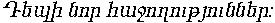
\includegraphics{images/armenian-closing}
\end{acknowledgments}

\begin{abstract}
write your abstract here
\end{abstract}

\tableofcontents

\hypersetup{pageanchor=true}
\mainmatter
\chapter{Introduction}
\label{chap:introduction}
This chapter gives the context and the purpose of the pipeline proposed in this thesis. It introduces unmanned aerial vehicles, the navigation systems they use to locate themselves, and the situations in which these systems can be interrupted or interfered with. At the end of the chapter, the scope of the thesis is defined and the outline of the following chapters is given.

\section{Unmanned Aerial Vehicles and navigation systems}
\label{sec:intro-uav}
Unmanned Aerial Vehicles (UAVs), otherwise known as drones, have become ordinary tools over the last decade. They are used in fields ranging from agriculture, urban development, infrastructure inspection and delivery to public safety, search and rescue, and military and intelligence operations. \citet{shakhatreh2019survey} estimate the civil drone market alone at more than 45 billion dollars, with civil infrastructure as the largest part. All of these operations depend on the drone knowing its position precisely throughout the flight. To achieve this, a drone fuses several sensors \citep{liu2025survey}:

\begin{itemize}
\item a receiver for Global Navigation Satellite Systems (GNSS), such as GPS, Galileo, GLONASS and BeiDou,
\item an inertial measurement unit (IMU), made of accelerometers and gyroscopes,
\item a magnetometer for heading,
\item a barometer for altitude.
\end{itemize}

GNSS gives an absolute position anywhere on Earth, but because it depends on signals from satellites, it is susceptible to interference or complete signal blockage \citep{liu2025survey}. The IMU measures accelerations and rotations at a high rate, so it gives the relative motion between GPS fixes, but its small errors add up over time (drift). In practice the two are fused: GPS corrects the drift of the IMU, and the IMU fills the gaps between GPS fixes. This combination is the most widely used for drone navigation, but it raises the question of what can replace GPS when its signal is missing or wrong.

Since most drones already carry a camera, it is natural to use it in such cases. Matching the camera image against a geo-referenced map gives an absolute position that does not depend on any outside signal. Couturier and Akhloufi \citeyearpar{couturier2024avl} call this absolute visual localization: the current view is compared with reference data, usually satellite imagery or aerial images from earlier flights. Unlike IMU-based navigation, an absolute position does not drift, since each image is located on its own.

The reference map can be satellite imagery or an aerial orthophoto, that is, an aerial photo corrected so that every pixel has a known ground position. Satellite imagery covers far larger areas but is coarser, while an aerial orthophoto is sharper but covers a smaller area \citep{couturier2024avl, durgam2024crossview}. Either can be years older than the flight, so the ground may have changed, and the system must work on images taken long after the map. This thesis uses an aerial orthophoto of Udine provided by the University of Udine, and satellite-scale maps are the natural next step. The pretrained networks used in the pipeline were not trained on this map, so the same method can be tested on other maps and at satellite scale. Whether it holds there is left as future work (Chapter~\ref{chap:conclusions}).

\section{Vulnerabilities: jamming, spoofing, signal loss}
\label{sec:intro-vulnerabilities}
GPS can fail in three ways: it can be jammed, spoofed or simply lost, and in each case the drone must rely on its other sensors. The root of the problem is that GPS signals arrive at the receiver extremely weak, at about $10^{-16}$~W ($-130$~dBm) \citep{pnt2010jamming, khan2021spoofing}. The National PNT Advisory Board compares this to someone in Los Angeles seeing the light of a 60~W bulb in New York \citep{pnt2010jamming}. In addition, civil GPS signals have no encryption or authentication, so a receiver has no way to verify that a signal is real \citep{khan2021spoofing}.

Jamming means broadcasting noise on the GPS frequencies so that the receiver can no longer decode the satellite signals \citep{couturier2024avl}. It is cheap and easy to perform: the simplest jammers plug into a car's cigarette lighter and block all GPS reception nearby, while stronger ones can cover tens of square miles \citep{pnt2010jamming}. A jammed drone, however, knows that it has lost GPS, so it can switch to another source of position.

Spoofing means transmitting fake GNSS signals so that the receiver computes a wrong position \citep{khan2021spoofing}. It is more dangerous than jamming, because the drone does not know that its position is wrong and keeps trusting GPS. In June 2012, at White Sands Missile Range, a team from the University of Texas at Austin used a GPS spoofer about 620~m away to take control of a small civil drone hovering under GPS control and force it downward \citep{kerns2014spoofing}. The test showed that spoofing can steer a drone, not only blind it.

GPS can also be lost without any attacker. Buildings, bridges and dense tree cover can block the satellite signals, while reflections from surfaces (multipath) and electromagnetic interference can corrupt them \citep{couturier2024avl, liu2025survey}. A blocked signal has the same effect as jamming, while a reflected one can give a wrong position, much like spoofing.

Without GPS, the drone is left with dead reckoning: estimating its position from the last known fix and the motion measured by the IMU. This can extend a flight for a short time \citep{szykula2025deadreckoning}, but the IMU's error grows quickly, cubically in time according to Couturier and Akhloufi \citeyearpar{couturier2024avl}, so it cannot give a reliable position for long. The aim of this thesis is therefore a pipeline that locates the drone using only what it already carries, its camera and an on-board map, without relying on any outside signal.

\section{Problem statement and contributions}
\section{Thesis outline}

\chapter{Background and related work}
\label{chap:background}
At the core of this project is the computer vision aspect of deep learning, specifically accurate feature detection, keypoint generation and subsequent matching. This allows us to decompose elements of the given scenery down to its minute details, to be used later as reference points for robust odometry. The feature extractors and matchers used in the pipeline introduced in this thesis rely on deep neural networks and descriptor vectors in order to achieve the highest accuracy without the need to retrain the matchers on new data every time. In this chapter we cover the tools and methods that went into creating the pipeline, which is described in detail in the later chapters.

\section{Feature extraction and matching}
\label{sec:bg-features}
SuperPoint~\citep{detone2018superpoint} is a self-supervised framework for training interest point detectors and descriptors to solve multiple-view geometry problems in computer vision. It is essentially a fully-convolutional model that processes full-sized images and computes pixel-level interest point locations and their associated descriptors in one forward pass. Its training uses Homographic Adaptation, a multi-scale, multi-homography approach for boosting interest point detection repeatability and cross-domain adaptation. Trained on the MS-COCO dataset \citep{lin2014coco} with this approach, it detects a much richer set of interest points than its initial, pre-adapted version and than traditional corner detectors, and it achieves state-of-the-art homography estimation compared with LIFT \citep{yi2016lift}, SIFT \citep{lowe2004sift} and ORB \citep{rublee2011orb}. For its state-of-the-art accuracy, efficiency, open-source access, and the absence of any need to retrain the model on a new dataset, it has been chosen as the core of one of the two visual odometry pipelines tested in this thesis.

SuperGlue~\citep{sarlin2020superglue} is a neural network whose purpose is to match two sets of local features by jointly finding correspondences and rejecting non-matchable points. The matches are found by solving a differentiable optimal transport problem, whose costs are predicted by a graph neural network. The uniqueness of the SuperGlue approach is that it introduces a flexible context aggregation mechanism, based on attention, which allows the network to reason about the underlying 3D scene and the feature assignments at the same time. Instead of relying on hand-designed heuristics, it learns priors about geometric transformations and the regularities of the 3D world from image pairs. It outperforms other learned approaches and achieves state-of-the-art results in pose estimation in both indoor and outdoor environments. In order to use the full capability of the system, SuperPoint was used as the feature detection network while SuperGlue played the role of the matcher.

The early experiments of the project, however, pointed to a serious setback in using the SuperPoint + SuperGlue system as it is: its computational cost is a concern for real-time performance on the limited hardware of a drone. For that reason, its better optimized and more lightweight successor, LightGlue, was selected.

LightGlue~\citep{lindenberger2023lightglue} is a deep neural network that revisits and improves SuperGlue. It requires less memory and computational power, it is more accurate, and it adapts to the difficulty of the given problem. On images with greater overlap, or with other visual features that make it easier to match common pairs of keypoints, it runs much faster, while on harder images it takes more time to analyze the keypoints correctly.

For the computer vision part of the pipeline, the logical alternative to a detector-based system, which first detects keypoints and then matches them, is a detector-free system, which matches the images directly. Hence LoFTR and its more lightweight successor EfficientLoFTR were selected for this project.

LoFTR~\citep{sun2021loftr} is a detector-free local feature matcher. It first establishes pixel-wise dense matches at a coarse level and later refines the good matches at a fine level. In contrast to dense methods that use a cost volume to search for correspondences, LoFTR uses self- and cross-attention layers in a Transformer to obtain feature descriptors that are conditioned on both images. The global receptive field of the Transformer allows the network to produce dense matches even in low-texture areas, where feature detectors usually struggle. At the time of its release, LoFTR outperformed state-of-the-art methods by a large margin.

EfficientLoFTR~\citep{wang2024efficientloftr}, as the name suggests, is a more efficient semi-dense alternative to its predecessor, based on an aggregated attention mechanism with adaptive token selection. A novel two-stage correlation layer is used to achieve accurate subpixel correspondences, resulting in higher accuracy. The model is about 2.5 times faster than the original LoFTR, and its efficiency can even surpass that of the SuperPoint + LightGlue pipeline. On paper, this made it a solid choice for our geo-localization pipeline. The tests, however, showed it to be unsuitable for this task, because rotation and changes in color and lighting each broke its matching (Chapter~\ref{chap:vo}).

\section{CNNs and image retrieval}
\label{sec:bg-retrieval}
A drone that has lost its position cannot match its image against the whole map, because the map is far too large for that. For that reason, the pipeline this thesis introduces first narrows the search down with image retrieval. A neural network turns every patch of the map into a short vector of numbers, a so-called fingerprint, and the camera image is turned into a fingerprint the same way. The patches whose fingerprints are most similar to that of the camera image become the candidates, and only those are checked with the feature matcher. In this section we cover the convolutional neural networks and the methods that went into this retrieval step, which forms the second stage of our pipeline (Chapter~\ref{chap:relocalization}).

This two-step approach is known as hierarchical localization \citep{sarlin2019hloc}. A global descriptor of the whole image first retrieves candidate locations from a database, and local features matched against those candidates then give the precise position. The advantage of this approach is that the feature matching, which is expensive in terms of computing time, runs only on a handful of candidates instead of the whole database, which makes it suitable for real-time use. The pipeline in this thesis follows the same scheme: a CNN fingerprint retrieves the candidates and SuperPoint + LightGlue verifies them.

Image retrieval for localization is studied in the field of visual place recognition, where the task is to recognize the location of a given photograph. NetVLAD is a CNN architecture for this task, trained end-to-end on Google Street View images taken at the same places at different times \citep{arandjelovic2016netvlad}. Its main component is the NetVLAD layer, which pools the features of the network into a single descriptor of the image and has to be trained for that purpose. It outperformed both non-learned image representations and standard CNN descriptors. NetVLAD also evaluates retrieval as the percentage of queries for which a correct location is among the top $N$ retrieved images, the equivalent of the Recall@$K$ used in this thesis. Since this project uses pretrained networks without fine-tuning, a layer that requires training could not be used, and the simpler global average pooling was used instead.

ResNet is a family of convolutional networks built on residual learning \citep{he2016resnet}. Instead of learning a mapping directly, each block of layers learns the difference, or residual, between its input and its output. This makes very deep networks much easier to train, so they can gain accuracy from depth rather than becoming harder to optimize. With this approach, ResNet won the ImageNet classification challenge of 2015 with networks of up to 152 layers. Its 50-layer version, ResNet50, has become the standard backbone of image retrieval, and with about 23.5 million parameters in its feature layers it was chosen as one of the two CNNs tested in this thesis.

The weights of a network depend on the data it was trained on, so the choice of pretraining matters as much as the architecture. Places is a database of 10 million photographs labeled with the type of scene they show \citep{zhou2018places}. Its Places365 version has 365 scene categories, and networks trained on it learn to describe whole scenes rather than single objects. Aerial images of fields, roads and buildings are much closer to scenes than to objects. Hence the ResNet50 used in this project carries the official Places365 weights.

EfficientNet, as the name suggests, focuses on the efficiency of convolutional networks \citep{tan2019efficientnet}. Its authors show that the depth, width and input resolution of a network should be scaled together, in a fixed balance, rather than one at a time. Its baseline network, EfficientNet-B0, was found through neural architecture search, and the larger versions B1 to B7 are scaled up from it. At the time of its release, the largest version reached state-of-the-art accuracy on ImageNet while being 8.4 times smaller and 6.1 times faster than the best existing network. EfficientNet-B0 has only about 4 million parameters in its feature layers. This is essential for the on-board computer of a drone, and for that reason it was chosen as the lightweight network of the two CNNs. Its weights come from ImageNet, a database of over a million photographs in 1000 object categories and the standard benchmark for image classification \citep{russakovsky2015imagenet}, since that is the only official pretraining available for it. Overall, it turned out to be the best of the three retrievers in this project, as the tests in Chapter~\ref{chap:relocalization} showed.

Both networks were originally built for classification, so their last layers, which output a class, were removed. What remains is a stack of feature maps, and these are turned into a single fingerprint with global average pooling, which averages each feature map into one number \citep{lin2014nin}. The result is a vector of 2048 numbers for ResNet50 and 1280 for EfficientNet-B0. Each vector is then normalized to a length of one, so that the similarity of two fingerprints can be measured simply by their dot product.

\section{Visual odometry and dead reckoning}
\label{sec:bg-vo}
Dead reckoning is one of the oldest navigation methods used in sailing. A ship's navigator estimates the current position from the last known position, the ship's speed and heading, and the time that has passed since that position was known. The same principle applies to a drone. Its main weakness is that every small error in the measured motion is added to the position and never removed, so the error grows the longer the drone flies without an external correction. This growth is called drift.

Szyku{\l}a and Furtak \citeyearpar{szykula2025deadreckoning} present a dead reckoning method for UAVs in conditions of limited GPS signal, based on the analysis of data from inertial measurement units (IMUs) and mathematical algorithms. The orientation of the drone is estimated from the gyroscope, accelerometer and magnetometer, and the acceleration is integrated over time to obtain the velocity and then the position. Tested on logs of real flights, the method accumulated errors of more than a hundred meters without GPS, while a GPS update every 15~s kept the error at about 12 to 22~m. The authors conclude that dead reckoning is effective for short durations and as a temporary complement to GPS, but not reliable for long flights without an external correction. They name wind as the main unresolved problem, since the sensors cannot tell the drone's motion through the air from its motion over the ground, and suggest optical flow as one possible solution.

Visual odometry solves the same problem with a camera instead. It is essentially the process of estimating the motion of a vehicle using only the images of one or more cameras attached to it \citep{scaramuzza2011vo}. The term was introduced by \citet{nister2004vo}, who estimated the motion of a single camera or a stereo camera pair in real time from video. Visual odometry works by comparing consecutive images, estimating the motion between them and adding that motion to the previous position. In other words, it is a form of dead reckoning in which the motion is measured by the camera, so it drifts in the same way. Its advantage over inertial dead reckoning is that a downward-looking camera sees the ground itself, so it measures the motion over the ground and is not affected by wind. Its limitation is that it needs enough light, texture and overlap between consecutive images.

In the visual odometry used in this thesis, the camera looks straight down at ground that is roughly flat, so between two images the view can only shift, rotate and change scale when the altitude changes. Every correct pair of keypoints matched by SuperPoint and LightGlue (Section~\ref{sec:bg-features}) must therefore follow the same transformation with four unknowns, a so-called similarity transform. Among the matches, however, some are always wrong, and they can disrupt the accuracy of the visual odometry estimate. For that reason, the transformation is estimated with RANSAC \citep{fischler1981ransac}. RANSAC repeatedly picks the smallest random set of matches that defines a model, two pairs in the case of a similarity, computes the model and counts how many of the other matches agree with it. The model with the most agreeing matches (the inliers) is kept. This makes the estimate robust even when a large part of the matches is wrong.

\section{Sensor fusion with the extended Kalman filter}
\label{sec:bg-ekf}
In this section we cover the extended Kalman filter (EKF), which is used in the third stage of our pipeline (Chapter~\ref{chap:ekf}) to combine the measurements of the previous stages into a single estimate of the drone's position.

The pipeline produces three kinds of measurements: the movement measured by visual odometry, the position given by a map check and the position found by relocalization. They differ in how much they can be trusted, and each of them has gaps that the others can cover. Combining measurements of different reliability into one estimate is called sensor fusion, and filtering is one of its main approaches \citep{liu2025survey}.

The Kalman filter \citep{kalman1960} keeps an estimate of the drone's position and velocity together with its uncertainty. In the prediction step, it moves the state forward in time with a model of the motion and increases the uncertainty. In the update step, it corrects the state with a new measurement, and the size of the correction depends on how certain the prediction and the measurement are: a precise map check moves the estimate a lot, while a noisy odometry step moves it only a little. The extended Kalman filter does the same for motion and measurements that are not linear, such as a drone that turns.

A filter can also take in measurements from an inertial measurement unit (IMU), which contains accelerometers and gyroscopes. An IMU on its own drifts quickly, since every small error is integrated over time \citep{szykula2025deadreckoning}, but combined with the camera it bridges the moments when vision fails, while the camera removes its drift. The reference point for this combination is VINS-Mono \citep{qin2018vinsmono}, which fuses a single camera with a low-cost IMU and was demonstrated in autonomous flight on board a small drone. Instead of a filter, it uses a nonlinear optimization over a window of recent frames, which is more demanding in computation. It also has no map, so it can only recognize places it has already visited. An EKF processes one measurement at a time, which suits both the step-by-step structure of our pipeline and the limited on-board computer of the drone. The flights available for this thesis do not include IMU recordings, so the EKF was tested both without an IMU and with a simulated one (Chapter~\ref{chap:ekf}).

\section{Related work}
\label{sec:bg-related}
Due to the volume of research in recent years directed towards the development of more and more advanced deep learning models, it is only logical that computer vision-based systems would be tested for drone geo-localization. This section covers a few examples of such systems, with our pipeline being a direct competitor to them in terms of efficiency and accuracy.

Finding where an image was taken by comparing it with a database of known places is studied in the field of visual place recognition. Over the last decade, the image descriptions used for this task have shifted from hand-crafted features to features learned by neural networks \citep{masone2021vpr}. When the query and the reference are seen from different viewpoints, such as a drone image and a satellite map, the task is called cross-view geo-localization. Its methods, datasets and open challenges are reviewed by \citet{durgam2024crossview}. The first benchmark for drones is University-1652, which contains images of 1652 university buildings seen from synthetic drones, satellites and ground cameras, and defines two tasks: locating a place from drone images and guiding a drone to a place shown in a satellite image \citep{zheng2020university}. The authors also analyze a variety of standard CNN features on it, the same kind of pretrained features used by the retrievers in this thesis.

Some of the earliest work used CNNs to recognize the district a drone is flying over from the look of its buildings \citep{amer2017urban}. \citet{nassar2018registration} went further by registering each camera frame against an image generated from the satellite map at the drone's estimated position and by refining the result with matched semantic shapes, an idea close to the map check of our pipeline. Cabrera-Ponce and Martinez-Carranza \citeyearpar{cabrera2022geoloc} instead trained a compact CNN to estimate the drone's position directly from a single image, with average errors of 2.8 to 6.1~m at more than 100 frames per second. Another approach sorts the satellite patches along the drone's trajectory, so that each frame only has to be matched against a short sequence of patches rather than the whole map \citep{wang2024seqmatch}.

The work closest to ours in its matching is \textit{Analysis of Deep Feature Matching Algorithms in UAV Visual Localization} \citep{prutyanov2024deepmatch}. It localizes a UAV in three degrees of freedom with pretrained SuperPoint and LightGlue, used without fine-tuning both for the short-term motion between frames and for matching frames against the map. It also shows that the two networks can refine the estimate of a less accurate localization method. Evaluated on an NVIDIA Jetson Orin Nano, it reached acceptable performance for real-time localization, using the same matcher and the same on-board computer as this thesis.

Other recent systems combine several of these components. \citet{walczak2025fusion} estimate the drone's motion from the optical flow of a downward-facing camera and its heading from the IMU, reaching average errors of about 11 to 60~m on real flights, since without a map nothing removes the drift. \citet{tang2025citylevel} match aerial images against a two-dimensional city map with a Vision Transformer and fuse the result with visual odometry and GNSS in a particle filter, which localized aerial images in real time over more than 1000~km$^2$ of four cities. Its structure, with retrieval against a map, odometry in between and a filter combining the two, is the closest to the pipeline of this thesis.

The newest direction is foundation models: networks trained on very large image collections whose features work for many tasks without fine-tuning. DINOv2 is the best-known example \citep{oquab2023dinov2}, and AnyLoc showed that its features, without any training for place recognition, work across urban, indoor, aerial and underwater environments \citep{keetha2023anyloc}. \citet{li2024crossview} kept DINOv2 frozen and trained only a small adapter for drone-to-satellite retrieval on University-1652, without any labeled image pairs. These works follow the same idea as this thesis, pretrained networks without fine-tuning, with a stronger network, and they are a natural next step for the retrieval stage (Chapter~\ref{chap:conclusions}).

\section{Autoencoder-based localization (Fabris)}
\label{sec:bg-fabris}
Finally, this section covers the work of Fabris at the University of Udine \citep{fabris2025thesis}. Its significance is that it is the starting point of this project, the baseline for the comparison of our system and the first relocalization method tested in this thesis (Chapter~\ref{chap:relocalization}). Its model was trained directly on the dataset used in this work.

The aim of his thesis was an algorithm that determines the position of a drone by comparing the images of its downward-facing camera with reference images of the area. The autoencoder must perform geo-localization in real time, while the drone is in the air. The reference is an orthophoto of the Rizzi district in Udine, provided by Insiel, with a resolution of $8400 \times 9000$ pixels covering about 751{,}045~m$^2$. The drone photos were taken with a DJI Phantom~4 Pro. Since the orthophoto was taken with a different camera, its colors were first corrected offline to match a photo from the drone, so that the drone's computer does not have to do it in flight. The corrected orthophoto is then divided into overlapping patches with a sliding window. The final configuration uses patches of $512 \times 512$ pixels with a stride of 256 pixels, a 50\% overlap, which gives 1054 patches. The GPS coordinates of each patch center are stored in a dictionary.

Not every patch is useful for localization. Areas without distinctive features, such as fields, forests or gravel, look alike and are easily confused. For that reason, Fabris trained a ResNet50 to classify patches as salient or non-salient on a manually labeled set, reaching 97.8\% test accuracy. He then removed the non-salient patches, which reduced the dataset by about 30\%. To make the images more robust to the differences between the two cameras, three additional channels are added to each image: the edges found by the Sobel and Canny detectors and the corners found by the Harris detector. The input of the network therefore has six channels.

The core of the system is the compression of each image into a short vector, so that the drone only has to compare vectors instead of full images. Three methods were compared on a test set of 42 drone photos: principal component analysis (PCA) found the correct patch for 17 of them, the best Vision Transformer for 21 and an autoencoder for 28. An autoencoder is a network made of an encoder, which compresses the image into a vector, and a decoder, which tries to rebuild the image from that vector. Training it to rebuild the images forces the encoder to keep their essential information. At inference only the encoder is used. Attempts to improve the architecture included attention layers, residual blocks, batch normalization, depth-wise convolutions, and replacing the loss function with SSIM, L1 or a triplet loss. However, none of them beat the results of the original design. The final encoder has four convolutional layers and produces a vector of 2048 numbers. The patches are compared with cosine similarity, which performed best among the tested measures. With this configuration, the system found the correct patch for 30 of the 42 test photos (71.4\%), and for 37 of them the correct patch was among the five most similar (88.1\%).

In flight, the system does not search the whole map for every image. It starts from the last known GPS position and then compares each new image only with the patches within two strides of the previous match, a $5 \times 5$ neighborhood. It returns to a search over the whole map only when the similarity falls below a threshold of 0.35. Fabris also linked the stride, the size of this neighborhood, the speed of the drone and the time between images: at 25~km/h, for example, one image has to be taken about every 4~s. On three real paths of 12, 9 and 17 images, the system identified every position correctly. A naive baseline that compares the raw images found only between 33\% and 71\% of them and needed about 6.6~GB of memory, against about 1.08~GB for the proposed system, most of which is the encoder itself.

The system relies on several assumptions, which Fabris defined at the beginning of his thesis. The starting position is known from GPS, the camera always faces north, and the drone flies at a fixed altitude, about 57~m according to his calculation from the patch size and the field of view of the camera. The drone is also assumed to move at constant speed and only along the axes of the patch grid, since a diagonal move ends between patch centers, where no patch matches. He also names areas without distinctive features and poor lighting as limitations. The system was tested only on a workstation, and testing on the drone's on-board computer, lower numerical precision, rotated images and several altitudes are named as future work. These assumptions are the starting point of Chapter~\ref{chap:relocalization}, where his model is tested inside our pipeline.

\chapter{Data and experimental setup}
\label{chap:data}
\section{Dataset}
\label{sec:dataset}
The initial dataset consisted of six geo-referenced orthophotos and 58 images taken from an actual flight sequence provided by the University of Udine, using a DJI Phantom~4 drone (camera FC330) \citep{dji2016phantom4}. The visual odometry benchmarks were tested on all six orthophotos. The later stages, specifically the autoencoder and convolutional neural network (CNN) retrievers and the extended Kalman filter (EKF) \citep{kalman1960}, used only one of them, tile 06611109, which covers the area of the real flight photos. Each orthophoto has dimensions of $9000 \times 8400$ pixels, which at 0.1~m/px covers an area of $900 \times 840$~m, in the coordinate system EPSG:25833 (ETRS89 / UTM zone 33N).

In his autoencoder, Fabris applied a saliency mask on the tiles in order to train the network more efficiently. However, our pipeline does not use the salient/non-salient selection: every patch of the grid enters the database, and the 747 salient patches are only used to reproduce Fabris's method as a baseline. As the on-board map we used the color-corrected version of the original orthophoto, on which Fabris's network was trained. The original orthophoto instead plays the role of the real world: the simulated camera image is cut from it. The on-board map has no usable geo-reference of its own, so the code assumes it sits on the same pixel grid as the original tile. That assumption was measured and holds, with an offset of about 0.02~px. The consequence is that the simulated camera and the map differ in color but are geometrically identical, pixel for pixel. This makes simulated matching easier than in reality, where a map and a later flight never line up exactly. It is also why simulated fixes can be accurate to a few millimeters when no photometric change is applied. Simulated accuracy should be read as a best case.

The flight photos were taken during the same flight from which the orthophoto was produced, so the map and the photos show the ground in the same light and season. Before the flight photos could be tested on the pipeline, they required four pre-processing steps:

\begin{enumerate}
\item The flight photos are brought to the map's resolution. A photo's ground size per pixel is its altitude multiplied by the sensor width, divided by the focal length times the image width. Each photo is resized from that value to 0.1~m per pixel, so that photo and map share the same scale and the matcher's scale bounds make sense. Written as a formula, with $h$ the altitude in meters, $w$ the sensor width (6.17~mm), $f$ the focal length (3.61~mm) and $W$ the image width in pixels (4000 for this camera), the ground size of one pixel is
\begin{equation}
  g = \frac{h \cdot w}{f \cdot W}
  \label{eq:gsd}
\end{equation}
and the photo is resized by the factor $g / 0.1$. With the median altitude of $h = 80.8$~m above take-off this gives $g = 3.45$~cm.

\item The scale is calibrated once, at the known start. The altitude in the metadata is measured from the take-off point rather than from the ground beneath the drone, so the first resize is slightly off. One map check on the first photo, where the start position is known, measures the remaining scale error, and every photo is corrected by that factor. The calibration found that the images were 1.119 times too large, so after calibration the photos sit about 72.3~m above the ground, and each one covers about $123 \times 92$~m ($1236 \times 927$~px).

\item The offset between GPS and the map is measured without letting any photo grade itself. GPS and the orthophoto disagree by a constant shift of a few meters. A map check on every photo, started 15~m away, measures that shift photo by photo, and the reference position of photo~$i$ is its GPS plus the median shift of the other 57 photos. This construction matters, because a photo scored against its own measurement would make the map check seem perfect. Over all photos, the offset between GPS and the map is 2.40~m to the west and 4.03~m to the south.

\item The photos are put in flight order by capture time, and the gimbal yaw serves as the compass. In flight order they are about 55~m apart (median 54.6~m, maximum 143.5~m). Six of the gaps are longer than 100~m, and the whole path is 3.5~km long. The gimbal yaw stays between $-2.3^\circ$ and $+0.1^\circ$ for the whole flight, so every photo is almost exactly north-up. The real flight photos therefore do not test robustness to rotation, only the simulation does.
\end{enumerate}

An important caveat of the dataset is that out of the 58 real flight photos, seven could not be matched to the map even at the correct position. These photos stay in the flight sequence, but at most 51 photos can be found by any retriever at later stages of the pipeline's test runs.

\section{Flight simulation and data augmentation}
\label{sec:simulation}
The flight simulations have two parts: a path and a render of the camera's view along it. The path is a seeded random walk, with each step being 205~px or 20.5~m long. For the visual odometry testing a flight of 512~m was simulated, while for the pipeline testing a flight of 2~km was simulated. In the visual odometry benchmarks there are two modes of flight operations: 4-connectivity (vertical, horizontal) and 8-connectivity (vertical, horizontal, diagonal). To test the complete pipeline we used five seeds, while for the visual odometry (VO) tests we used 10 seeds per configuration.

Each flight starts at a random position at least 82~m from the edge of the tile, so that every camera crop stays inside the image. The drone starts facing north at its nominal altitude, which is the only pose it is told. In the code this is the attitude matrix $G$ equal to the identity, $G = I$. A straight step moves 20.5~m, so two consecutive images share 80\% of their area. A diagonal step moves 20.5~m along both axes at once, which is 29~m, and the two images then share only 64\% of their area ($0.8 \times 0.8$). A 25-step flight is 512~m with 4-connectivity and about 600~m with 8-connectivity. The smaller overlap is the main reason diagonal paths produce more failed steps.

The camera's current view is generated on the fly. A 1640~px crop of the world orthophoto is cut around the drone's position, rotated by the drone's heading and rescaled by its scale factor. The central $1024 \times 1024$~px images are then kept (102.4~m ground area). This is the final crop dimension used for the pipeline. This size is large enough to contain hundreds of SuperPoint \citep{detone2018superpoint} keypoints even over fields, and it matches the size of a real flight photo after resizing (about 1230~px wide). Generating the initial crop with larger dimensions guarantees that the $1024 \times 1024$~px patch does not have fillers caused by the rotations (blank pixels). A 1024~px square rotated by any angle needs a square of $1024 \times \sqrt{2} \approx 1448$~px to stay filled, and at the smallest scale of 0.9 it needs $1448 / 0.9 \approx 1609$~px. The 1640~px crop is the next convenient size above that (8 steps of 205~px).

\subsection{Patch grids and image sizes}
\label{sec:patch-grids}
Besides the 1024~px camera image, the system uses one more image size. The database of the on-board map is built from patches of 512~px (51.2~m), the same size Fabris used. His autoencoder was trained on patches of this size, so the comparison has to keep it for the autoencoder to be treated fairly. Fabris's grid places a patch every 256~px (25.6~m), giving 1054 patches, 747 of which passed his saliency filter. Our pipeline uses a dense grid with a patch every 64~px (6.4~m), giving 16{,}492 patches. On a 25.6~m grid, a position can be up to 18.1~m from the nearest patch center, and the real flight photos lie about 10.8~m away on median. On a 6.4~m grid, no position is more than 4.5~m from a center. To measure this, crops of the color-corrected on-board map and of the raw orthophoto were cut at a given offset from 200 patch centers, without any rotation or scale change, and the test counted how often the nearest patch was ranked first (top-1) or among the first five (top-5). Table~\ref{tab:offset-retrieval} shows how quickly the autoencoder's retrieval accuracy falls as the query moves away from the nearest patch center: with the color-corrected map, top-1 accuracy stays above 96\% up to an offset of 3.2~m but drops to 37.5\% at 6.4~m. The reason this matters is shown in Chapter~\ref{chap:relocalization}. The dense grid is used for every retriever, so the comparison between them stays fair, and searching all 16{,}492 fingerprints costs only a matrix product of a few milliseconds.

\begin{table}[!htbp]
  \centering
  \caption{Offset tolerance of Fabris's autoencoder}
  \label{tab:offset-retrieval}
  \begin{tabular}{rrrrrr}
    \toprule
    \multicolumn{2}{c}{Offset} & \multicolumn{2}{c}{Color-corrected map} & \multicolumn{2}{c}{Raw orthophoto} \\
    \cmidrule(lr){1-2}\cmidrule(lr){3-4}\cmidrule(lr){5-6}
    px & m & Top-1 & Top-5 & Top-1 & Top-5 \\
    \midrule
      0 &  0.0 & 100.0\% & 100.0\% & 76.5\% & 78.5\% \\
      8 &  0.8 &  99.0\% &  99.0\% & 76.0\% & 80.5\% \\
     16 &  1.6 &  98.5\% &  99.0\% & 72.0\% & 79.5\% \\
     32 &  3.2 &  96.0\% &  98.0\% & 48.0\% & 65.5\% \\
     64 &  6.4 &  37.5\% &  58.0\% &  7.5\% & 14.0\% \\
     96 &  9.6 &  13.0\% &  25.5\% &  0.5\% &  3.5\% \\
    128 & 12.8 &   8.5\% &  15.5\% &  0.5\% &  4.5\% \\
    \bottomrule
  \end{tabular}
\end{table}

\subsection{Augmentations and test scenarios}
\label{sec:augmentations}
The augmentations are applied dynamically, on the 1640~px crops as they are being generated, rather than being stored as a dataset. For testing, we defined five conditions:

\begin{enumerate}
\item \textbf{None}: applies no change and serves as a control.
\item \textbf{Rotation}: the heading is changed by $[-15^\circ, +15^\circ]$ per image and the changes accumulate over time.
\item \textbf{Scale}: the scale changes by $[-10\%, +10\%]$ per image, as the altitude varies.
\item \textbf{Photometric}: the Albumentations library \citep{buslaev2020albumentations} applies color jitter (contrast and brightness changes by $[-30\%, +30\%]$, saturation by $[-20\%, +20\%]$, hue shifts by $[-5\%, +5\%]$), Gaussian noise (standard deviation of $[5\%, 15\%]$ of the intensity range, the same on all three channels) and motion blur (kernel range $[5, 15]$~px).
\item \textbf{Realistic}: this setting combines all the above mentioned augmentations in order to achieve the most realistic flying conditions.
\end{enumerate}

The variation in the applied augmentation on the images was created deliberately in order to test how the matchers and retrievers behave given specific test conditions. However, all the flights in the final system were run in the `realistic' condition. Each image has its own random seed, derived from the flight seed and the frame number ($\text{seed} \times 1000 + \text{frame}$). The rendered images are also cached, so every method compared on a flight sees exactly the same pixels.

The compass is simulated as the true heading plus Gaussian noise of $3^\circ$. It is not used in visual odometry. It is used only to rotate relocalization queries north-up, which is a prerequisite for the retriever networks, since none of them are rotation-invariant.

Three scenarios test the pipeline:

\begin{enumerate}
\item \textbf{Long flight}: regular flight sequence, nothing goes wrong.
\item \textbf{Camera blackout}: simulates conditions of vision loss from the drone. In the final tests, frames 40--51 (12 frames, about 250~m) return nothing to the localizers.
\item \textbf{Unknown start}: the drone is told a start 200--400~m from the truth in a random direction and does not know it is wrong.
\end{enumerate}

In the performance comparisons the blackout is placed on a straight leg, while in the EKF testing the blackout is placed both on a straight leg and on a leg with blind turns. In the blackout on a straight leg, the path repeats its last step for the 12 blind frames, so the drone flies about 250~m in one direction. In the unknown start, the direction of the wrong start is drawn uniformly, and its distance uniformly between 200 and 400~m, and the drone's uncertainty is set to infinity, so its first fix has to be a search of the whole map. Fabris's own method, in contrast, is always started from the correct patch when the start is known.

In the EKF testing, the drone flies a smooth curve (cubic spline) through the waypoints at 5~m/s, close to the speed of the real flight (about 50~m between photos, about 12~s apart). That gives one image every 4.1~s, with the inertial measurement unit (IMU) sampled at 100~Hz along the same curve. The curve's peak acceleration is checked against what a Phantom~4 can physically do without GPS: in ATTI mode (attitude mode, without GPS position hold) its maximum tilt of $35^\circ$ \citep{dji2016phantom4} allows about 6.9~m/s$^2$. The peak acceleration over all simulated paths is 5.01~m/s$^2$, which is inside that limit.

\section{Evaluation metrics}
\label{sec:metrics}
The metrics are the core of the evaluation, since they measure the accuracy with which the drone estimates its location in comparison with the reference position (which the drone never sees). The metrics are divided into three categories. Speed is measured only on the final pipeline and is described together with its results in Section~\ref{sec:jetson-runtime}.

\subsection{Odometry and flight accuracy}
\label{sec:metrics-odometry}
The final error is how far the estimated position is from the reference at the last image. This is an essential metric for visual odometry, but it can hide a flight that went far off in the middle and came back. That is why the ATE (absolute trajectory error) is reported next to it, the root mean square of the error over all images except the first, which exposes exactly those detours in the middle of a flight. On one of the tiles, for example, the median final drift was 0.83~m but the median ATE 4.04~m (Section~\ref{sec:vo-failures}). The maximum error captures the worst moment of the flight, which is what matters during a blackout. The share of images within 5~m of the truth says how much of the flight was usable, and a flight counts as recovered if it ends within 5~m.

With the estimated position $\hat{p}_k$ and the true position $p_k$ at image $k$, and $N$ images after the first, the trajectory error is
\begin{equation}
  \mathrm{ATE} = \sqrt{\frac{1}{N}\sum_{k=1}^{N} \lVert \hat{p}_k - p_k \rVert^2}
  \label{eq:ate}
\end{equation}

The cause of a failure is found by the VO benchmark, since it also measures each step on its own. The step translation error compares one measured movement with the true movement starting from the keyframe, converted with the true attitude so that it isolates this single measurement. The step rotation error does the same for the measured rotation. The final heading error is how far the tracked heading has drifted by the end of the flight. Three numbers describe the matching itself: the number of matches per step, the inlier ratio (the share of matches that agree with the fitted motion) and the reprojection error of the inliers in pixels. A failed step is one whose measurement was rejected by the 15-inlier or scale rule. Drift is also reported as a percentage of the path length.

\subsection{Retrieval quality}
\label{sec:metrics-retrieval}
These metrics measure the extent to which the retriever found the correct location. Recall@$K$, where $K = 1$, 5 and 10, is the share of queries for which one of the top $K$ candidates lies within 18.1~m of the truth. The threshold of 18.1~m is half the diagonal of a 25.6~m cell, so a hit roughly means landing in the right cell of Fabris's grid. Recall@5 matters most, because the pipeline verifies five candidates. The top-1 error (median and mean) and the share of top-1 candidates within 5, 10, 50 and 100~m describe how far the best guess lands.

Recall alone says nothing about whether the pipeline can use a candidate, so two verification metrics complete the picture. A correct fix is a fix whose best LightGlue-verified candidate has at least 50 agreeing matches and lies within 5~m of the truth. If a candidate cannot be verified it is never used. A false fix is a candidate that passed verification while being more than 5~m off, in other words a wrong position accepted as right. Finally, the gate sweep repeats the verification with minimum-match thresholds from 15 to 150 and reports accepted, correct and false fixes. It shows whether the threshold of 50 is a safe choice.

\subsection{Filter consistency}
\label{sec:metrics-filter}
These metrics measure the extent to which the drone is aware of how lost it is. The truth-in-radius share is the fraction of images on which the true position lies inside the search radius, so if the metric scores low, the drone is searching in the wrong area. It is reported for both the rule-based pipeline and the EKF.

The remaining two apply to the EKF only. NEES (normalized estimation error squared) \citep{barshalom2001} is $e^{\top} P^{-1} e$, where $e$ is the true position error and $P$ the filter's position covariance. For a two-dimensional position its average should be about 2: above 2 the filter is overconfident, below 2 it is too cautious. The share of images with NEES under 5.99 (the 95\% bound) should be about 95\%. The number of fixes rejected by the $\chi^2$ gate shows how often the filter refused a measurement. For image $k$, with the position error $e_k$ and the $2 \times 2$ position block $P_k$ of the filter's covariance,
\begin{equation}
  \mathrm{NEES}_k = e_k^{\top} P_k^{-1} e_k, \qquad e_k = \hat{p}_k - p_k
  \label{eq:nees}
\end{equation}

\chapter{Visual odometry}
\label{chap:vo}
Visual odometry is the drone's sense of its own motion. Similar to dead reckoning in a ship's position estimation through its recorded speed and heading, visual odometry carries the position forward from one image to the next one. The drone only knows where it started and for every new image, it asks how far it moved and how it turned since the last keyframe (good image) and adds that motion to its estimate.

\section{Methodology}
\label{sec:vo-method}
Since the camera looks straight down at the ground that is roughly flat, between two images the view can only slide, rotate and change scale (when the altitude changes). Tilt and perspective effects are negligible. Every correct pair of matched points must therefore obey a single rule with four unknowns, a 4-degree-of-freedom similarity transform, otherwise known as 4-DOF.

As described in Section~\ref{sec:simulation}, the overlap between two consecutive images was set to 80\%, meaning visual matchers had reliable room to detect the movement between two frames. Each step works as follows. SuperPoint \citep{detone2018superpoint}, a CNN, finds up to 2048 keypoints in each image at distinctive features of the frame and describes each one of those keypoints with a vector. LightGlue \citep{lindenberger2023lightglue}, an attention-based matcher, pairs the keypoints generated by SuperPoint in the given pair of images. RANSAC (random sample consensus) \citep{fischler1981ransac} then finds the similarity hidden among the matches: for up to 50{,}000 iterations it takes two random pairs, computes the rule they imply and counts how many other pairs agree within 5~px. OpenCV \citep{bradski2000opencv} stops earlier once it is confident that a better rule is unlikely to be found. The rule with the highest number of agreeing pairs (inliers) wins. The step is accepted only if at least 15 pairs agree and the scale change lies between 0.5 and 2, since a drone cannot halve or double its altitude between two images. Both SuperPoint and LightGlue are used with their pretrained weights and the similarity is fitted with OpenCV's \texttt{estimateAffinePartial2D}, which estimates exactly these four parameters. Two pairs are enough to define a similarity, so a model supported by only a handful of pairs can arise by chance. Requiring at least 15 agreeing pairs rules that out.

Since the camera looks straight down, the center of each image is the point directly beneath the drone, so the drone's movement is where the center of the new image lies in the keyframe, relative to the keyframe's center: $d = A^{-1}(c - t) - c$, with $c$ the image center. The drone therefore keeps a running attitude $G$ (scale and rotation from map to image) and converts the movement into map directions before adding it, $P \leftarrow P + G^{-1} d$. It then updates the attitude with the rotation and scale just measured, $G \leftarrow A\,G$. The new image becomes the keyframe.

When a step fails, the drone keeps track of its last estimate and last good keyframe, comparing the new image to the latest valid keyframe. To make sure no ground truth leaks into this estimate, the code was tested with a matcher that returns no matches, and the estimate never left the start.

The step can be described using the following formulas:
\begin{align}
  p_{\mathrm{new}} &= A\,p_{\mathrm{key}} + t, \qquad A = s\,R(\theta) \label{eq:vo-model}\\
  d &= A^{-1}(c - t) - c \label{eq:vo-move}\\
  P &\leftarrow P + G^{-1} d, \qquad G \leftarrow A\,G \label{eq:vo-update}
\end{align}
The first is the fitted model, the second is the movement of the drone in keyframe pixels and the third is the update of position and attitude.

To verify the implementation of these formulas, we performed checks on three cases with known answers, on images without photometric change. The expected answers are a shift of 205~px east, a rotation of $-10^\circ$ and a scale of 1.1. Table~\ref{tab:vo-known-answer} lists the expected values next to what each matcher measured, with shifts in pixels and the inlier ratio as the share of matches that agree with the fitted motion. In this and the following tables, SP+LG stands for SuperPoint + LightGlue and ELoFTR for EfficientLoFTR \citep{wang2024efficientloftr}.

\begin{table}[!htbp]
  \centering
  \caption{Known-answer checks of the odometry step}
  \label{tab:vo-known-answer}
  \small
  \begin{tabular}{llrrrrr}
    \toprule
     & & Shift & Shift & Rotation & & Inlier \\
    Test & & east (px) & south (px) & ($^\circ$) & Scale & ratio \\
    \midrule
    Moved 205~px east & Expected & 205 & 0 & 0 & 1 & -- \\
     & SP+LG & 205.012 & $-0.008$ & 0.000 & 1.000 & 0.996 \\
     & ELoFTR & 208.000 & 0.000 & 0.000 & 1.000 & 1.000 \\
    \addlinespace
    Stationary, & Expected & 0 & 0 & $-10$ & 1 & -- \\
    \quad heading $10^\circ$ & SP+LG & 0.013 & 0.040 & $-9.999$ & 1.000 & 0.994 \\
     & ELoFTR & 41.772 & 8.283 & $-19.807$ & 1.002 & 0.045 \\
    \addlinespace
    Stationary, & Expected & 0 & 0 & 0 & 1.1 & -- \\
    \quad scale 1.1 & SP+LG & 0.009 & 0.017 & 0.002 & 1.100 & 0.990 \\
     & ELoFTR & $-1.246$ & 0.106 & 0.147 & 1.100 & 0.496 \\
    \bottomrule
  \end{tabular}
\end{table}

LightGlue recovers all three with an accuracy of at most a few hundredths of a pixel. EfficientLoFTR handles the shift and the scale approximately (it measures the 205~px shift as 208~px), but for a pure $-10^\circ$ rotation it reports $-19.8^\circ$ and a false shift of 42~px, with under 5\% of its matches agreeing.

\section{EfficientLoFTR vs SuperPoint + LightGlue}
\label{sec:vo-matchers}
The matcher was chosen by the benchmarks. Each one of the six tiles was flown with 10 seeds, two matchers and two path types (4- and 8-connectivity, described in Section~\ref{sec:simulation}), giving 240 flights of 25 steps (512~m with 4-connectivity, about 600~m with 8-connectivity) in the realistic condition. SuperPoint + LightGlue was accurate at every level: each step was off by about 27~cm and $0.04^\circ$. At the flown distance, the median final drift was 0.64~m with 4-connectivity, about 1~m per 800~m flown, and 0.89~m with 8-connectivity. EfficientLoFTR on the other hand, as a detector-free transformer-based matcher, produced about four times more matches, but only about 2\% of them agreed with a single motion, whereas with LightGlue this metric was at 74\%. EfficientLoFTR's rotation error was about $6.5^\circ$ per step, which accumulated in the stored heading, so every later movement was added in the wrong direction, resulting in the drone getting lost. Many matches are worthless if they do not agree with one motion and a rotation error is far more significant than a shift error, because it bends the whole remaining path.

Both matchers were given the same images and the same estimator, so only the matching differed. EfficientLoFTR was the pretrained version from the HuggingFace Transformers library \citep{wolf2020transformers}, run at native 1024~px resolution without resizing, since the internal stride of the model accepts image dimensions of size divisible by 32. Matches were kept with a confidence of at least 0.2, the default. Higher thresholds, from 0.4 to 0.9, were also tried on a test flight and did not rescue the matcher: the final drift stayed between 5 and 35~m. The pooled results over all six tiles, 60 flights per matcher and connectivity, are shown in Table~\ref{tab:vo-pooled}.

\begin{table}[!htbp]
  \centering
  \caption{Pooled visual odometry benchmark}
  \label{tab:vo-pooled}
  \small
  \begin{tabular}{lrrrr}
    \toprule
     & \multicolumn{2}{c}{4-connectivity} & \multicolumn{2}{c}{8-connectivity} \\
    \cmidrule(lr){2-3}\cmidrule(lr){4-5}
    Metric & SP+LG & ELoFTR & SP+LG & ELoFTR \\
    \midrule
    Final drift, median (m) & 0.64 & 82.28 & 0.89 & 84.24 \\
    Final drift, mean (m) & 0.82 & 91.00 & 3.44 & 88.03 \\
    Final drift, std (m) & 0.61 & 53.27 & 11.34 & 54.54 \\
    Drift (\% of path) & 0.12 & 16.05 & 0.15 & 14.30 \\
    ATE, median (m) & 0.57 & 61.33 & 0.68 & 59.63 \\
    ATE, mean (m) & 1.21 & 66.02 & 4.08 & 66.59 \\
    Step translation error, median (m) & 0.27 & 5.38 & 0.28 & 5.46 \\
    Step rotation error ($^\circ$) & 0.04 & 6.51 & 0.04 & 6.62 \\
    Final heading error ($^\circ$) & 0.27 & 30.53 & 0.28 & 27.14 \\
    Matches per step & 694 & 2958 & 635 & 2939 \\
    Inlier ratio & 0.738 & 0.021 & 0.719 & 0.019 \\
    Reprojection error (px) & 2.34 & 2.92 & 2.34 & 2.91 \\
    Failed steps & 11/1500 & 609/1500 & 56/1500 & 583/1500 \\
    \bottomrule
  \end{tabular}
\end{table}

For SuperPoint + LightGlue, the error of a single step is nearly the same on every tile, 0.26--0.29~m, so the matcher itself does not depend on the terrain. Table~\ref{tab:vo-per-tile} breaks the same flights down by tile, with 10 flights per tile and configuration, and its step error is the median step translation error. As visible from the table, tile 06611109 with diagonal movements had the most failed steps of this matcher, 51. Since at this stage of the pipeline visual odometry's estimate is not supported by any other system, a single failure can cause a completely wrong localization of a whole flight. On these flights the mean final drift is 11.3~m, although the median is 1.4~m. A single lost flight can distort the mean as an outlier in this way, which is why medians are also reported in the table.

\begin{table}[!htbp]
  \centering
  \caption{Visual odometry results per tile}
  \label{tab:vo-per-tile}
  \small
  \setlength{\tabcolsep}{4pt}
  \begin{tabular}{llcrrrrrr}
    \toprule
     & & & \multicolumn{2}{c}{Final drift (m)} & ATE (m) & Step & Inlier & Failed \\
    \cmidrule(lr){4-5}
    Tile & Method & Conn. & median & mean & median & error (m) & ratio & steps \\
    \midrule
    06611109 & SP+LG & 4 & 0.72 & 1.05 & 0.63 & 0.28 & 0.729 & 1/250 \\
     & ELoFTR & 4 & 69.04 & 83.68 & 45.83 & 5.17 & 0.021 & 68/250 \\
     & SP+LG & 8 & 1.37 & 11.26 & 4.95 & 0.29 & 0.601 & 51/250 \\
     & ELoFTR & 8 & 50.55 & 64.01 & 47.27 & 4.98 & 0.023 & 129/250 \\
    \addlinespace
    06611110 & SP+LG & 4 & 0.72 & 0.84 & 0.51 & 0.27 & 0.779 & 0/250 \\
     & ELoFTR & 4 & 88.77 & 76.39 & 50.19 & 6.07 & 0.015 & 51/250 \\
     & SP+LG & 8 & 0.73 & 0.75 & 0.49 & 0.27 & 0.779 & 0/250 \\
     & ELoFTR & 8 & 104.70 & 94.66 & 83.70 & 6.69 & 0.017 & 65/250 \\
    \addlinespace
    06611112 & SP+LG & 4 & 0.60 & 0.79 & 0.52 & 0.27 & 0.725 & 0/250 \\
     & ELoFTR & 4 & 78.75 & 96.30 & 61.83 & 5.06 & 0.021 & 95/250 \\
     & SP+LG & 8 & 0.97 & 1.00 & 0.71 & 0.27 & 0.726 & 1/250 \\
     & ELoFTR & 8 & 77.88 & 89.17 & 55.44 & 5.06 & 0.020 & 93/250 \\
    \addlinespace
    06611113 & SP+LG & 4 & 0.44 & 0.48 & 0.38 & 0.27 & 0.757 & 0/250 \\
     & ELoFTR & 4 & 84.97 & 98.08 & 64.67 & 5.38 & 0.020 & 130/250 \\
     & SP+LG & 8 & 0.52 & 0.78 & 0.56 & 0.28 & 0.769 & 0/250 \\
     & ELoFTR & 8 & 106.85 & 99.14 & 66.73 & 5.67 & 0.016 & 109/250 \\
    \addlinespace
    06611114 & SP+LG & 4 & 0.70 & 0.70 & 0.51 & 0.27 & 0.767 & 1/250 \\
     & ELoFTR & 4 & 81.83 & 84.40 & 66.19 & 5.01 & 0.019 & 97/250 \\
     & SP+LG & 8 & 1.08 & 0.99 & 0.64 & 0.28 & 0.760 & 1/250 \\
     & ELoFTR & 8 & 70.59 & 90.10 & 46.40 & 4.89 & 0.017 & 60/250 \\
    \addlinespace
    06611116 & SP+LG & 4 & 0.83 & 1.06 & 4.04 & 0.26 & 0.672 & 9/250 \\
     & ELoFTR & 4 & 107.28 & 107.16 & 81.37 & 6.40 & 0.028 & 168/250 \\
     & SP+LG & 8 & 1.17 & 5.83 & 0.84 & 0.28 & 0.680 & 3/250 \\
     & ELoFTR & 8 & 67.92 & 91.09 & 55.01 & 4.97 & 0.022 & 127/250 \\
    \bottomrule
  \end{tabular}
\end{table}

For both of the matchers the performance was also measured for the different augmentation conditions discussed in Section~\ref{sec:augmentations}. Three seeded flight simulations were performed (tile 06611109, seeds 26, 42 and 77), with 25 steps each (75 in total) and in the 4-connectivity mode. The only condition that hurts LightGlue is the photometric one: its drift rises to about 1~m and its inlier ratio falls from 99\% to 75\% (Table~\ref{tab:vo-ablation}, where drift is the final drift and the rotation error is the step rotation error). The realistic condition gives the same numbers, so LightGlue's error in realistic flights is photometric, not geometric.

\begin{table}[!htbp]
  \centering
  \caption{Augmentation ablation of the two matchers}
  \label{tab:vo-ablation}
  \small
  \begin{tabular}{lrrrrrrrr}
    \toprule
     & \multicolumn{4}{c}{SP+LG} & \multicolumn{4}{c}{ELoFTR} \\
    \cmidrule(lr){2-5}\cmidrule(lr){6-9}
    Condition & Drift & Inlier & Rot.\ err. & Failed & Drift & Inlier & Rot.\ err. & Failed \\
     & (m) & ratio & ($^\circ$) & steps & (m) & ratio & ($^\circ$) & steps \\
    \midrule
    None & 0.05 & 0.988 & 0.003 & 0/75 & 2.54 & 0.895 & 0.000 & 0/75 \\
    Rotation & 0.11 & 0.986 & 0.004 & 0/75 & 129.17 & 0.061 & 7.726 & 7/75 \\
    Scale & 0.03 & 0.984 & 0.002 & 0/75 & 8.25 & 0.539 & 0.044 & 0/75 \\
    Photometric & 0.97 & 0.754 & 0.033 & 0/75 & 25.99 & 0.045 & 0.209 & 11/75 \\
    Realistic & 0.96 & 0.730 & 0.037 & 0/75 & 54.01 & 0.017 & 4.940 & 16/75 \\
    \bottomrule
  \end{tabular}
\end{table}

EfficientLoFTR has two separate weaknesses. Rotation alone is catastrophic, since only 6\% of its matches agree and the rotation error causes a drift of 129~m. Photometric change alone also breaks the matcher, in a different way: only 4.5\% of the matches agree. Scale alone is tolerable (8~m). However, even with no change it drifts about 2.5~m, far more than LightGlue's 0.05~m.

Figures~\ref{fig:vo-flight} and~\ref{fig:vo-matches} demonstrate these results on a simulated flight. The first one shows one flight (tile 06611109, seed 26, 4-connectivity), with frame-to-frame odometry on the left and matching against the map on the right. Its upper panels show the trajectories of both matchers and its lower panels their error against the distance flown. The second figure shows what each matcher matched on one step of the simulated flight.

\begin{figure}[!htbp]
  \centering
  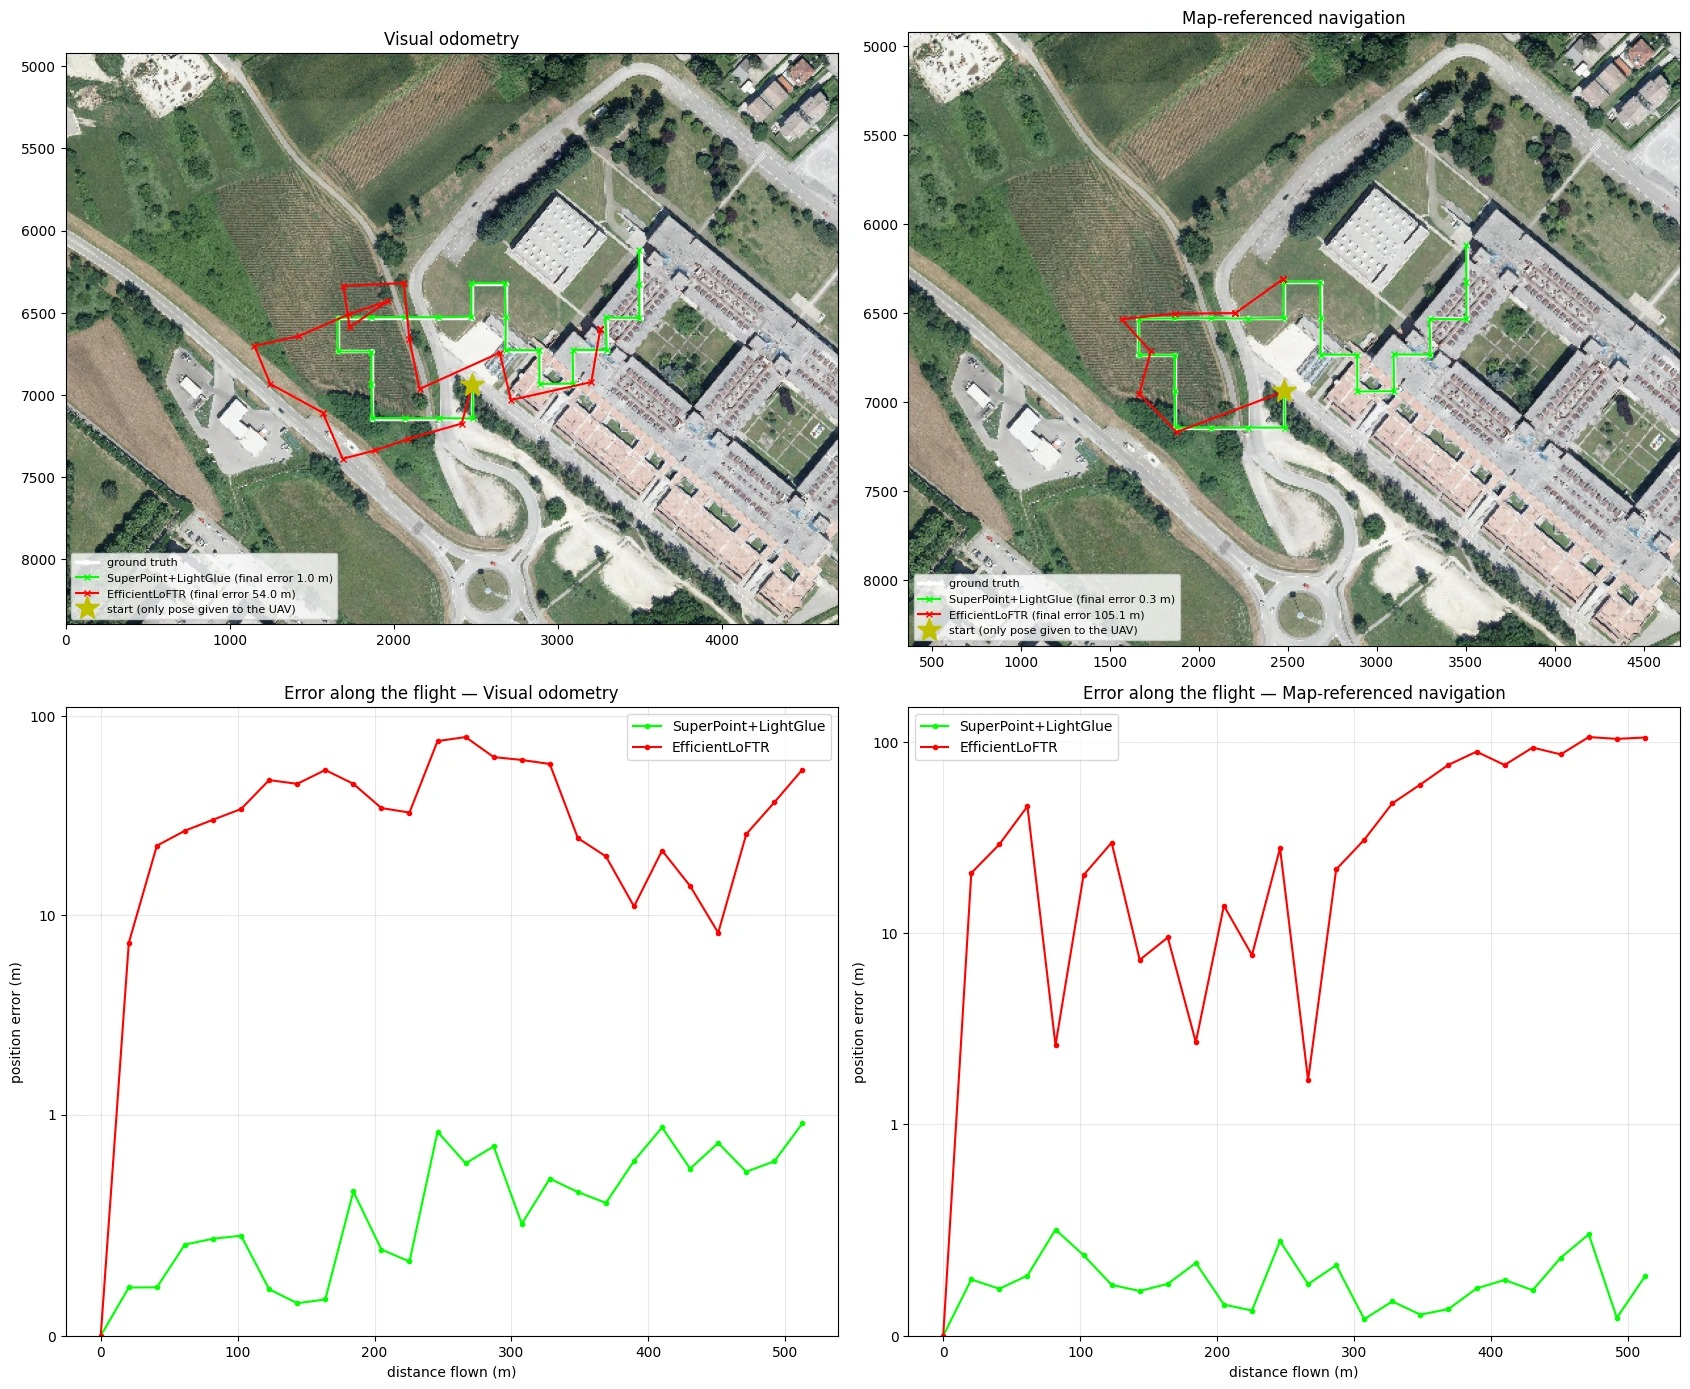
\includegraphics[width=0.85\textwidth]{images/vo-flight-seed26.jpg}
  \caption{One simulated flight with both matchers}
  \label{fig:vo-flight}
\end{figure}

In Figure~\ref{fig:vo-flight}, green denotes the position error of LightGlue while red denotes the position error of EfficientLoFTR. Clearly, LightGlue follows the true path, its error rising slowly with distance to 1.0~m at the end. EfficientLoFTR on the other hand leaves the path within the first steps and ends approximately 54~m off. When each image is matched against the map, LightGlue's error no longer grows. It stays below 0.5~m and ends 0.3~m off. That is precisely the reason the pipeline uses map checks every once in a while.

\begin{figure}[!htbp]
  \centering
  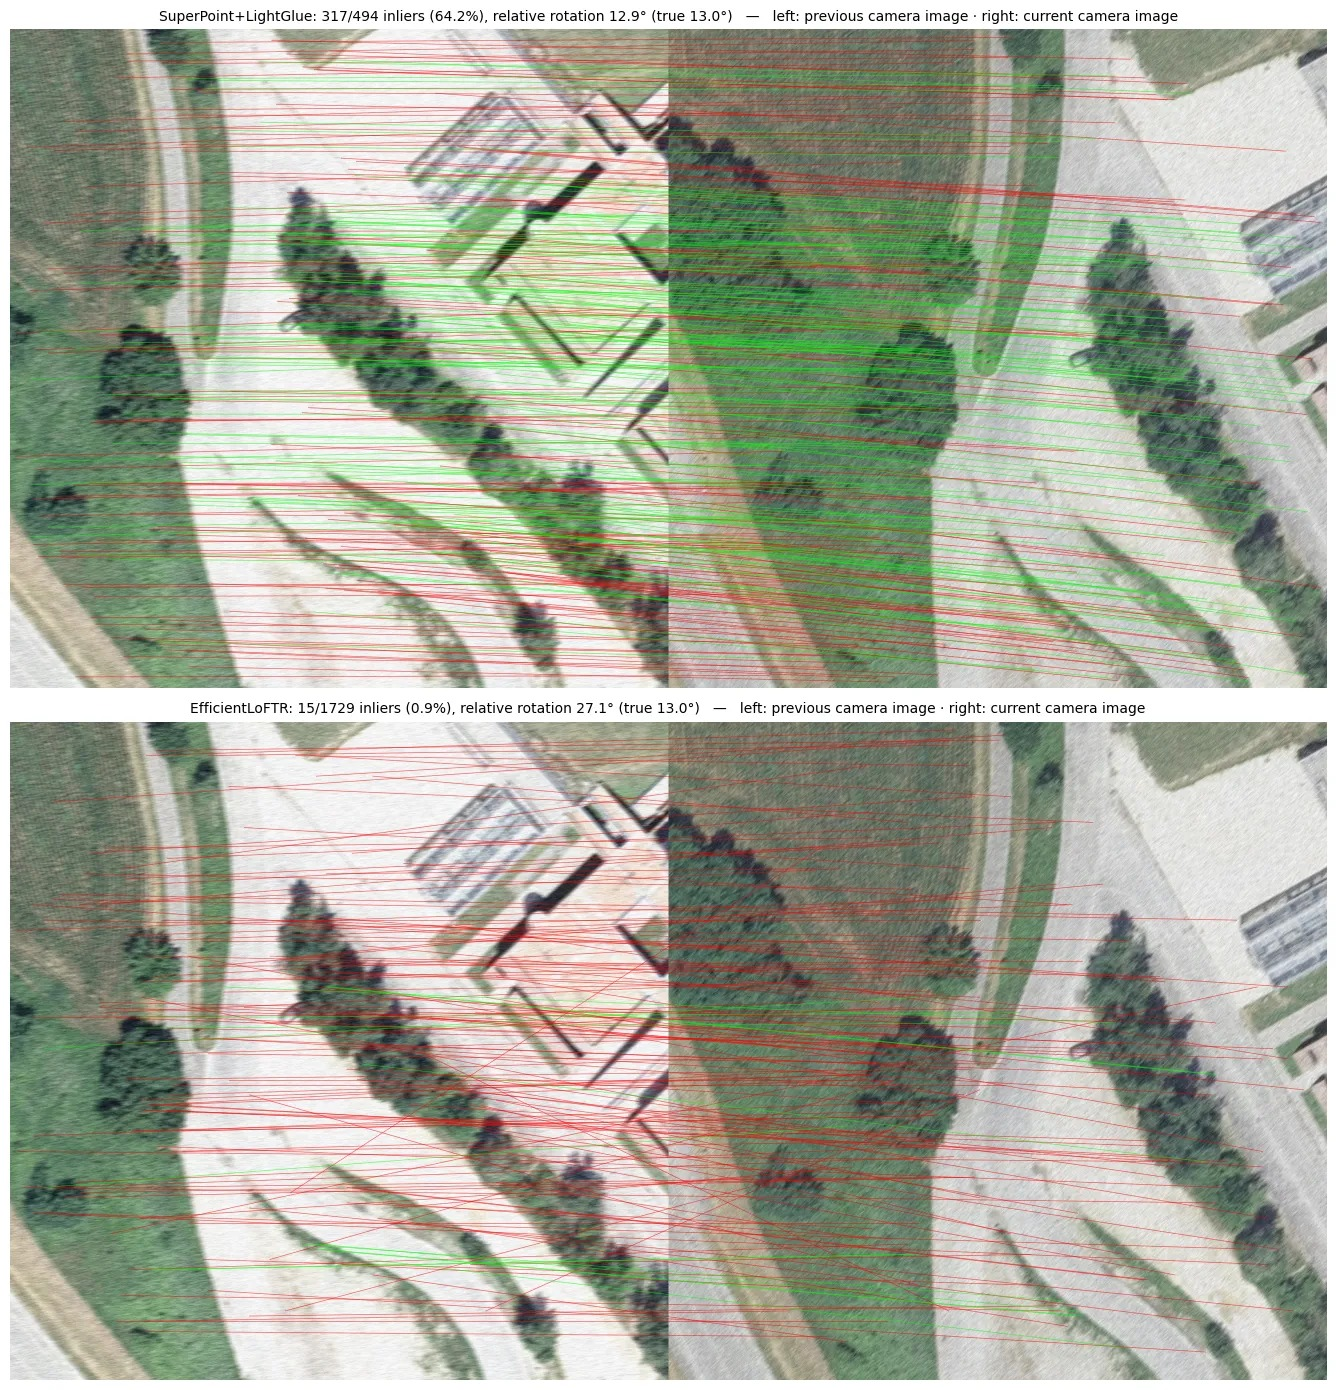
\includegraphics[width=0.62\textwidth]{images/vo-matches-step.jpg}
  \caption{Matches of both matchers on one step}
  \label{fig:vo-matches}
\end{figure}

Figure~\ref{fig:vo-matches} shows SuperPoint + LightGlue on top and EfficientLoFTR below, with accepted matches in green and rejected ones in red. On this step, with a true rotation of $13.0^\circ$, LightGlue estimated $12.9^\circ$ with 317/494 matches accepted, while EfficientLoFTR estimated $27.1^\circ$ with 15/1729 accepted.

\section{Failure modes and drift}
\label{sec:vo-failures}
The benchmark also revealed how odometry fails. Of the 56 of 1500 failed steps on diagonal paths, 51 were on tile 06611109, whose flights start over fields with rows of nearly identical texture, where matched points are ambiguous. After a failure the drone keeps its last good keyframe, but the gap to it widens with every step, and once the images no longer overlap, odometry has no way of recovering. A flight can also go far off in the middle and come back. On tile 06611116 (4-connectivity), the median final drift was 0.83~m while the median ATE was 4.04~m, which is why both numbers are reported. Figure~\ref{fig:vo-failed} shows an instance of a failed flight (tile 06611109, seed 42, 8-connectivity, realistic condition), laid out like Figure~\ref{fig:vo-flight}, in which LightGlue ended 81.8~m off the track. Matching against the map cannot rescue this flight either, because once the estimate is more than about 30~m off over repetitive fields, the map crop no longer shows the right place.

\begin{figure}[!htbp]
  \centering
  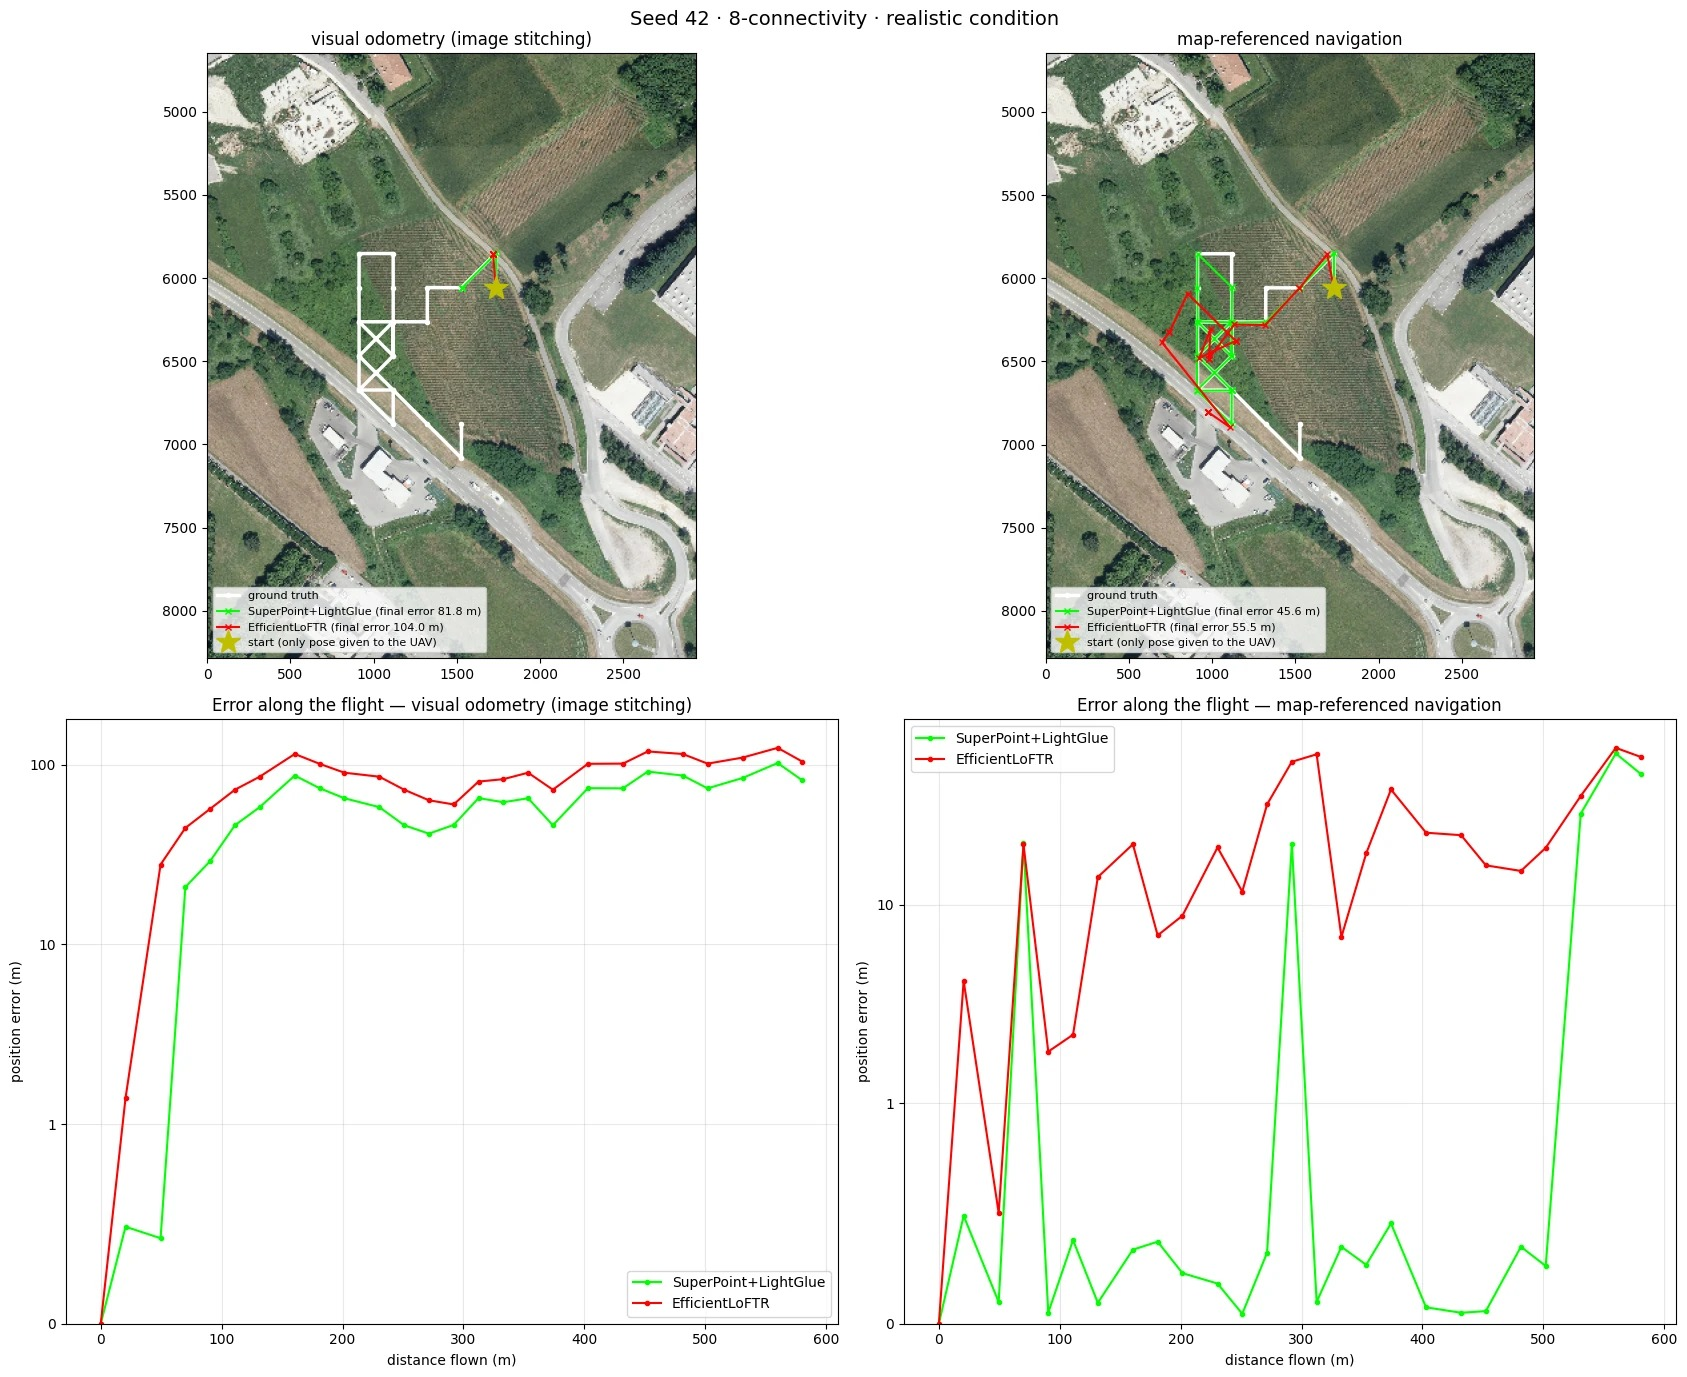
\includegraphics[width=0.85\textwidth]{images/vo-failed-seed42.jpg}
  \caption{A failed flight over fields}
  \label{fig:vo-failed}
\end{figure}

This leads to two conclusions about visual odometry:
\begin{enumerate}
\item Odometry is accurate locally but accumulates drift and cannot recover from a failure by itself. Matching against the map removes that drift, so the pipeline needs map checks, and, for an estimate that is already too far off, relocalization.
\item EfficientLoFTR should be dropped in favor of SuperPoint + LightGlue in later experiments and in the final system.
\end{enumerate}

\section{Map checks}
\label{sec:map-check}
Visual odometry measures change, but the drone carries a map which gives the absolute position. A map check asks whether the current image matches the map at the place where the drone believes it is, and if so, where exactly. The map check is run every 5th image and in cases where the odometry fails. Checking more often would cost time for no gain. The check cuts a 1024~px piece of the on-board map, north-up centered on the estimated location. Since SuperPoint + LightGlue is not rotation-invariant, the images have to look the same way so the image is de-rotated and rescaled with the drone's current attitude $G$. LightGlue then matches the map crop with the de-rotated and rescaled image, and RANSAC fits the same kind of similarity as in odometry, from map to camera.

In map checks the acceptance rules are stricter than in VO: at least 50 pairs must agree, the scale must lie between 0.67 and 1.5 since the altitude is known and the image is brought to map scale. When the fix is accepted, the position becomes crop center + measured offset, $G$ the measured transform. Both position error and heading error are therefore removed at once. The check can only work if the true view still overlaps the crop, which holds while the estimate is within about 30~m of the truth.

Two details complete the description. The crop is centered on the estimate rounded to a whole pixel. LightGlue works on the de-rotated image, but the matched points are converted back to the raw camera image with $G$ before RANSAC runs, so the fitted transform is the full map-to-camera attitude and replaces $G$ directly.

The effect of map checks can be seen in the VO (odometry alone) and VO+map (odometry with map checks) rows of Table~\ref{tab:reloc-all-sim} (five simulated flights of 2~km per scenario) and Table~\ref{tab:reloc-all-real} (the real photo flight). Both tables also contain the full pipelines of Chapter~\ref{chap:relocalization}.


Clearly, on a normal flight it removes the drift almost entirely: the drone ends a median 0.18~m from the truth after 2~km and its largest error is a median 0.74~m, so relocalization is never needed. Tested alone on the real photos from 15~m off, it located 51 of 58 photos with a median error of 1.2~m. It cannot, however, bring back a drone that is already far off. After the blackout the estimate is about 250~m behind, so the map crop shows the wrong place and almost every check fails, and only one of the five flights recovers. With a wrong start it never succeeds at all. On the real photos only 7 of 25 attempts succeeded, because after each long gap the estimate was too far off. The map check therefore keeps a drone on track but cannot find a lost one. That gap is filled by relocalization.

\chapter{Relocalization}
\label{chap:relocalization}
\section{Why it is needed}
\label{sec:reloc-why}
Even though the upgrade of the initial pure visual odometry with map checks increases the likelihood of the drone geo-localizing itself accurately, there are still situations where the odometry can fail: a camera blackout (fog, glare, a covered lens, a jammed video link), a break in the odometry across a long gap between images, or a wrong start. When that happens, a big gap is left in the estimate of the position, leading to a potentially unrecoverable drift in the drone's position estimates. To address these issues, the system needs a complete relocalization through the means of analyzing the whole map, or at least a large area. The problem not only requires an accurate estimate, but also a solution that would be reasonable to execute on a drone that needs relocalization in real time.

Checking every place on the map with LightGlue \citep{lindenberger2023lightglue} would take minutes. Each patch of the map is summarized before the flight by a fingerprint vector and during the flight, the current image's fingerprint is compared with all of them within milliseconds, so that only a few most similar places need checking with LightGlue.

To decide when to run the relocalization sequence, the drone keeps an uncertainty value $r$, which denotes how far off it believes it could be. It starts at 1~m with a known start and at infinity when it does not know where it started. It grows by 1~m for every successful odometry step and by 25~m (about 1.2 times the 20.5~m step, an upper bound on how far the drone can move in one frame) for every image without measurement, either a blackout or a failed odometry step, and it returns to 1~m after any accepted fix. On every 5th image or when odometry fails the value of $r$ is checked: if it is at most 30~m a map check is performed, and if it is larger a relocalization is performed. If a map check fails while odometry worked, the drone waits for the next scheduled fix. If odometry also failed, or it is the second failed map check in a row, the estimate is no longer trusted: $r$ is raised to at least 60~m and a relocalization sequence is run on the same image.

As an example, consider a blackout in which the drone encounters 12 blind frames, so nothing can be measured. The uncertainty grows to about 300~m. When the camera returns, the keyframe is still the last image from before the blackout, about 250~m behind. So the odometry finds no overlap and fails. The uncertainty is above 30~m, so the relocalization sequence is attempted within the uncertainty radius. It succeeds, the position and the attitude are replaced, the image becomes the new keyframe and odometry resumes on the next frame. The drone is therefore back on track at the first image after the blackout, which is what the results show.

The relocalization sequence itself works the same way for every retriever. The query is the camera image de-rotated with the compass heading and the current scale estimate, and its central 512~px is kept, which corresponds to the map patch dimensions. Instead of using the tracked heading, which most likely is wrong due to loss in camera footage, the compass of the drone is used. The query's fingerprint is compared with every patch fingerprint by cosine similarity. The five most similar places are taken, each at least 25.6~m from the others so that they are five different places rather than five neighboring patches of the same place. At first, they are drawn within $r + 51.2$~m of the estimate and if none of them pass, five new ones are drawn from the whole map. Each candidate is verified with a full map check centered on it, using the same 50-match rule. The candidate with the most agreeing pairs wins. The retriever only proposes the patches and LightGlue decides which ones are valid.

\section{Fabris's autoencoder with VO}
\label{sec:reloc-ae}
The autoencoder proposed by Fabris takes a 512~px patch with six channels: three color channels, Sobel edge magnitude, Harris corner response and Canny edge strength. Four strided convolutional layers and one linear layer compress it into a 2048-number fingerprint for 269 million parameters in total, almost all of them in the final linear layer. Fabris's approach was to localize each image independently, by taking the top-1 patch among the 747 previously identified salient patches of the 25.6~m grid and using that patch's center as the position, searching $\pm 2$ grid cells around the previous match first when that match was confident (requires a similarity of at least 0.35).

In our relocalization pipeline, Fabris's autoencoder is used exactly as it is: using the same weights, patches, locations. The construction is the following: four convolutions have $3 \times 3$ kernels and a stride of 2, with 64, 128, 128, 128 channels and a ReLU after each. Each one of those halves the image, turning the 512~px into a 32~px image. Thus $128 \times 32 \times 32 = 131{,}072$ values are mapped by the linear layer onto 2048. The Harris channel is rescaled to the range 0--1 separately for each image. The sixth channel is the Canny edge-strength map. Processing the patches in batches was checked to give the same fingerprints as processing them one by one, with cosine similarity of 1.

The autoencoder had to be reproduced true to his thesis, in order to test its performance fairly. On the 38 of his 42 test crops that could be located on the map, our reproduction reached 68.4\% top-1 and 84.2\% top-5, against the 71\% and 88\% reported in his thesis, meaning the encoder is reproduced faithfully.

However, on the real photos the autoencoder's top-1 candidate was the right patch for only about 5\% of the photos on his grid. The reason behind the seeming underperformance is the test crops themselves: the centers of the crops lie a median 1.4~m from the patch center, while the centers of the real photos lie a median of 10.8~m from the nearest patch center. The shift table (Table~\ref{tab:offset-retrieval}) shows that the autoencoder recognizes a place reliably only within about 3~m, so his tests measured a nearly ideal case. This is the reason for the 6.4~m dense grid implementation.

To understand this gap and to choose the density of the grid, we performed a series of tests:
\begin{itemize}
\item Exact crops of the color-corrected map were shifted by 0 up to 12.8~m from a patch center, without any rotation or scale change (200 patches per offset). The top-1 rate stays at 96\% up to 3.2~m from the patch center, but falls to 37.5\% at 6.4~m.
\item The same crops were cut from the raw orthophoto, to isolate the effect of color. The top-1 rate fell from 100\% to 76.5\% at zero offset, meaning that the encoder is also sensitive to the color correction it was trained with.
\item His 42 hand-made test crops were located on the map with LightGlue (38 succeeded) and passed through his own pipeline with his saved fingerprints. Those crops cover about 52~m and their centers lie a median of 15.6~m from the center of the photo they were cut from.
\end{itemize}
In other words, the test crops were cut to line up with the patches, whereas the center of a real photo does not. On the 6.4~m grid, no position is more than 4.5~m from a patch center.

Finally, the autoencoder was built into the pipeline as the relocalization step. Its results are in the rows VO+map, +AE (VO+map with the autoencoder as the relocalization step) and AE only (Fabris's original method) of Table~\ref{tab:reloc-all-sim} (simulated flights) and Table~\ref{tab:reloc-all-real} (the real photo flight), both given in full in Section~\ref{sec:reloc-comparison}.

In the simulated flights, the autoencoder managed to recover two scenarios, where after the blackout and from a wrong start it relocalizes the system within 0.2~m from the actual location. Without it, the odometry + map checks stayed 175--272~m off. It is important to note that the maximum error of 246~m during the blackout is not a failure of localization. It is simply caused by the absence of data from the drone's camera. Fabris's autoencoder on its own ends 170--270~m off, because a single unverified top-1 guess per image is wrong too often.

On the real photos, the autoencoder found 28/58 photos on the dense grid, 11/58 on his grid, with no wrong fix (Table~\ref{tab:retrieval-real}). Flown as one flight, the retriever relocalized the drone at three of the four gaps where odometry broke, 1--2~m from the GPS. At the last gap, the retriever found no verified place, so the flight ended 194.6~m off. Overall, the estimation was within 5~m for 69\% of the photos, against 45\% with map checks only and 7\% with visual odometry alone.

The autoencoder works. However, its narrow tolerance to offset and the fact that it was trained on a single map are reasons to explore other retrievers.

\section{Pretrained CNN retrievers}
\label{sec:reloc-cnn}
The search for a new retrieval network had to fill the following gaps: a network that would not need retraining on every new map, a network that would be at least as accurate as the autoencoder and potentially better, a network that would require less computational power without losing accuracy. For those reasons, two convolutional neural networks were chosen: ResNet50 \citep{he2016resnet} and EfficientNet-B0 \citep{tan2019efficientnet}.

ResNet50 is the standard backbone of image retrieval and the baseline of the University-1652 drone-to-satellite benchmark \citep{zheng2020university}. It has about 23.5 million parameters and it has been pretrained on Places365 \citep{zhou2018places}, a dataset of scenes rather than objects, which is closer to aerial views of fields, roads and buildings than ImageNet \citep{deng2009imagenet}. The official MIT CSAIL checkpoint is used.

EfficientNet-B0 represents the potentially lightweight solution to the given problem. It has about 4 million parameters in its feature layers and its weights come from ImageNet.

Both networks are used the same way, which is the standard recipe for turning a classification network into a retrieval network. The classification head is removed and the network is run up to its last convolutional layer. The resulting feature map is averaged over all positions (global average pooling) into one vector of 2048 numbers for ResNet50 and 1280 for EfficientNet-B0. The vector is then L2-normalized, so that the dot product of two fingerprints equals their cosine similarity. Global average pooling has a property that explains much of the result: it summarizes what is in the patch more than where it is, so a patch shifted by a few meters keeps nearly the same fingerprint. The 512~px patch is resized to 224~px and normalized with the ImageNet mean and standard deviation, because a network pretrained at 224~px performs best at the size and statistics it was trained on. At 224~px one pixel covers about 0.23~m, which is still finer than most of the structures that identify a place.

In terms of implementation, both networks come from the torchvision library \citep{torchvision2016}. ResNet50 is cut after its last convolutional block, dropping its own pooling and classification layers. For a 224~px input that block outputs a $7 \times 7$ map with 2048 channels. EfficientNet-B0 is used through its features part, which outputs a $7 \times 7$ map with 1280 channels. Averaging the 49 positions gives the fingerprint. The patch is shrunk from 512 to 224~px with area interpolation, which averages the pixels it merges and so avoids aliasing. All ResNet50 results reported here use the Places365 weights. Everything else is kept identical to the autoencoder retriever: the same 512~px patches, both grids, the same de-rotation of the query with the compass, the same top-5 with 25.6~m spacing, the same LightGlue verification with the 50-match rule, and the same flights and photos. Only the fingerprint function changes, so any difference in the results is caused by the retriever alone.

\section{Comparison}
\label{sec:reloc-comparison}
At this stage, all of the available 58 real flight photos were searched from scratch, without any additional information to the retrievers. The top 5 candidates were verified by LightGlue. Table~\ref{tab:retrieval-real} reports the retrieval metrics of Section~\ref{sec:metrics-retrieval} for every retriever on both grids: Recall@$K$, the median distance of the top-1 candidate and the share of top-1 candidates within 5~m. The column `found' counts the correct LightGlue-verified fixes, and the fix error is the median error of those fixes.

\begin{table}[!htbp]
  \centering
  \caption{Real flight photos searched from scratch}
  \label{tab:retrieval-real}
  \footnotesize\setlength{\tabcolsep}{3.5pt}
  \begin{tabular}{llrrrrrrrr}
    \toprule
    & & & & & Top-1 & Top-1 & & False & Fix \\
    Retriever & Grid & R@1 & R@5 & R@10 & err.\ (m) & ${\le}5$~m & Found & fixes & err.\ (m) \\
    \midrule
    AE & 25.6~m & 0.05 & 0.09 & 0.10 & 410.6 & 0.03 & 11/58 & 0 & 1.31 \\
     & 6.4~m & 0.38 & 0.45 & 0.48 & 259.4 & 0.34 & 28/58 & 0 & 1.16 \\
    \addlinespace
    ResNet50 & 25.6~m & 0.38 & 0.66 & 0.74 & 23.4 & 0.05 & 44/58 & 0 & 1.19 \\
     & 6.4~m & 0.55 & 0.67 & 0.81 & 15.3 & 0.14 & 47/58 & 0 & 1.15 \\
    \addlinespace
    EffNet-B0 & 25.6~m & 0.47 & 0.66 & 0.71 & 19.0 & 0.07 & 44/58 & 0 & 1.20 \\
     & 6.4~m & 0.66 & 0.76 & 0.81 & 10.7 & 0.19 & 47/58 & 0 & 1.18 \\
    \bottomrule
  \end{tabular}
\end{table}

The test results indicate that the CNNs manage to find 47/58 photos on the dense grid while the autoencoder finds only 28/58. Since only 51 photos can be matched to the map at all (Section~\ref{sec:map-check}), the CNNs locate 92\% of the photos that can be found (47/51). The gap is even wider on Fabris's original grid: 44/58 for the CNNs while that number collapses to 11/58 for the autoencoder. Recall@1 favors EfficientNet-B0, 0.66 against 0.55, but after verification the two CNNs are equal, because LightGlue picks the right candidate whenever it is anywhere in the top 5. Importantly, no retriever produced a single false fix, which confirms that LightGlue verification protects the pipeline regardless of the proposed candidates.

The two CNNs each find 47 photos, but not the same 47. Both miss the seven unmatchable photos and three more (DJI\_0062, DJI\_0072 and DJI\_0078). In addition, EfficientNet-B0 misses DJI\_0079 and ResNet50 misses DJI\_0052. However, two of the photos that EfficientNet-B0 does not find from scratch, DJI\_0072 and DJI\_0079, are found during the flight, where the search starts near the estimate. Thus, a rough prior position helps retrieval, which is why the pipeline searches locally before it searches the whole map. The same comparison on 100 simulated queries per condition shows where each retriever is strong.

The simulated benchmark is built as follows. For each of the five conditions 100 query positions are drawn at random over the area covered by patch centers and the camera image is rendered there. In the conditions with rotation, the heading is drawn from the full circle, $-180^\circ$ to $180^\circ$, so the retriever is tested on any orientation. The query is then de-rotated with the simulated compass ($3^\circ$ of noise) and assumed to be at nominal altitude, so the $\pm 10\%$ scale change is unknown to the retriever. Every retriever receives the same query image. The top 10 candidates give the recall figures, and the top 5 are verified with LightGlue. The full results, with the same metrics on both grids, are given in Table~\ref{tab:retrieval-sim}.

\begin{table}[!htbp]
  \centering
  \caption{Simulated retrieval benchmark}
  \label{tab:retrieval-sim}
  \footnotesize\setlength{\tabcolsep}{3.5pt}
  \begin{tabular}{lllrrrrrrr}
    \toprule
    & & & & & & Top-1 & Top-1 & \multicolumn{2}{c}{Verified fix} \\
    \cmidrule(lr){9-10}
    Condition & Retriever & Grid & R@1 & R@5 & R@10 & err.\ (m) & ${\le}5$~m & correct & false \\
    \midrule
    None & AE & 25.6~m & 0.05 & 0.08 & 0.10 & 334.8 & 0.03 & 0.22 & 0.00 \\
     & AE & 6.4~m & 0.45 & 0.71 & 0.79 & 166.9 & 0.41 & 0.74 & 0.00 \\
     & ResNet50 & 25.6~m & 0.85 & 0.99 & 1.00 & 11.9 & 0.11 & 1.00 & 0.00 \\
     & ResNet50 & 6.4~m & 0.94 & 0.99 & 0.99 & 4.0 & 0.65 & 1.00 & 0.00 \\
     & EffNet-B0 & 25.6~m & 0.86 & 1.00 & 1.00 & 11.1 & 0.12 & 1.00 & 0.00 \\
     & EffNet-B0 & 6.4~m & 0.99 & 0.99 & 0.99 & 3.0 & 0.74 & 1.00 & 0.00 \\
    \addlinespace
    Rotation & AE & 25.6~m & 0.10 & 0.17 & 0.20 & 304.9 & 0.08 & 0.31 & 0.00 \\
     & AE & 6.4~m & 0.43 & 0.67 & 0.74 & 145.2 & 0.41 & 0.70 & 0.00 \\
     & ResNet50 & 25.6~m & 0.80 & 0.97 & 0.97 & 11.3 & 0.14 & 1.00 & 0.00 \\
     & ResNet50 & 6.4~m & 0.97 & 0.99 & 1.00 & 3.9 & 0.63 & 1.00 & 0.00 \\
     & EffNet-B0 & 25.6~m & 0.86 & 0.96 & 0.99 & 11.2 & 0.14 & 1.00 & 0.00 \\
     & EffNet-B0 & 6.4~m & 0.99 & 1.00 & 1.00 & 3.4 & 0.77 & 1.00 & 0.00 \\
    \addlinespace
    Scale & AE & 25.6~m & 0.05 & 0.11 & 0.11 & 319.5 & 0.04 & 0.22 & 0.00 \\
     & AE & 6.4~m & 0.37 & 0.61 & 0.74 & 223.6 & 0.35 & 0.67 & 0.00 \\
     & ResNet50 & 25.6~m & 0.80 & 0.99 & 1.00 & 12.3 & 0.09 & 1.00 & 0.00 \\
     & ResNet50 & 6.4~m & 0.92 & 0.99 & 0.99 & 4.4 & 0.55 & 1.00 & 0.00 \\
     & EffNet-B0 & 25.6~m & 0.82 & 0.99 & 0.99 & 12.3 & 0.11 & 1.00 & 0.00 \\
     & EffNet-B0 & 6.4~m & 0.96 & 1.00 & 1.00 & 3.5 & 0.69 & 1.00 & 0.00 \\
    \addlinespace
    Photometric & AE & 25.6~m & 0.08 & 0.17 & 0.21 & 323.2 & 0.05 & 0.39 & 0.01 \\
     & AE & 6.4~m & 0.69 & 0.78 & 0.82 & 3.5 & 0.62 & 0.83 & 0.00 \\
     & ResNet50 & 25.6~m & 0.35 & 0.62 & 0.70 & 40.5 & 0.04 & 0.75 & 0.00 \\
     & ResNet50 & 6.4~m & 0.43 & 0.65 & 0.75 & 24.4 & 0.10 & 0.77 & 0.00 \\
     & EffNet-B0 & 25.6~m & 0.58 & 0.85 & 0.88 & 14.6 & 0.10 & 0.92 & 0.00 \\
     & EffNet-B0 & 6.4~m & 0.74 & 0.87 & 0.89 & 10.1 & 0.25 & 0.94 & 0.00 \\
    \addlinespace
    Realistic & AE & 25.6~m & 0.15 & 0.27 & 0.32 & 283.4 & 0.11 & 0.45 & 0.00 \\
     & AE & 6.4~m & 0.61 & 0.72 & 0.80 & 3.9 & 0.54 & 0.75 & 0.00 \\
     & ResNet50 & 25.6~m & 0.31 & 0.64 & 0.72 & 45.5 & 0.07 & 0.76 & 0.00 \\
     & ResNet50 & 6.4~m & 0.50 & 0.70 & 0.80 & 20.6 & 0.14 & 0.82 & 0.00 \\
     & EffNet-B0 & 25.6~m & 0.53 & 0.75 & 0.81 & 16.9 & 0.11 & 0.89 & 0.00 \\
     & EffNet-B0 & 6.4~m & 0.66 & 0.89 & 0.90 & 8.3 & 0.25 & 0.94 & 0.00 \\
    \bottomrule
  \end{tabular}
\end{table}

The four augmentation conditions show which kind of change hurts which retriever. Each cell of Table~\ref{tab:retrieval-conditions} gives Recall@1, Recall@5 and the share of correct verified fixes on the dense grid.

\begin{table}[!htbp]
  \centering
  \caption{Effect of each augmentation condition on the dense grid}
  \label{tab:retrieval-conditions}
  \small
  \begin{tabular}{lccc}
    \toprule
    Condition & AE & ResNet50 & EfficientNet-B0 \\
    \midrule
    None & 0.45 / 0.71 / 0.74 & 0.94 / 0.99 / 1.00 & 0.99 / 0.99 / 1.00 \\
    Rotation & 0.43 / 0.67 / 0.70 & 0.97 / 0.99 / 1.00 & 0.99 / 1.00 / 1.00 \\
    Scale & 0.37 / 0.61 / 0.67 & 0.92 / 0.99 / 1.00 & 0.96 / 1.00 / 1.00 \\
    Photometric & 0.69 / 0.78 / 0.83 & 0.43 / 0.65 / 0.77 & 0.74 / 0.87 / 0.94 \\
    Realistic & 0.61 / 0.72 / 0.75 & 0.50 / 0.70 / 0.82 & 0.66 / 0.89 / 0.94 \\
    \bottomrule
  \end{tabular}
\end{table}

Evidently, the geometric changes do not affect the performance of the CNNs at all: with rotation or scale alone they reach a correct verified fix on every query. What costs them accuracy is the photometric change. From the conducted tests it is clear that ResNet50 loses more than EfficientNet-B0, keeping 77\% correct verified fixes against 94\%, even while having substantially more parameters.

It is interesting to observe that the autoencoder behaves the other way around and one of its results is not explained: it scores higher with photometric change than with no change at all (0.69 against 0.45). Two facts may contribute: the query positions differ between conditions, and the unchanged camera image comes from the raw orthophoto, whose colors the encoder was not trained on. Neither was tested as the cause, so this remains an open observation.

At the same time, it should be stated that when the autoencoder is right it is very precise: in the realistic condition its top-1 lands within 5~m for 54\% of the queries, against 25\% for EfficientNet-B0, because it was trained on this exact map and its fingerprint is sharp at the patch center. The CNNs are less precise but far more robust and they put the right area in their top 5 much more often (0.89 against 0.72, for EfficientNet-B0 and the autoencoder). Considering the fact that there was no fine-tuning involved for the CNNs and they operate with the pretrained weights, they have the potential to perform even more accurately given appropriate fine-tuning, which is left for future work.

Since after the retrieval step LightGlue measures the exact position anyway, robustness is what matters when it comes to retrievers and the verified-fix rate in the realistic condition reflects that: 94\% for EfficientNet-B0, 82\% for ResNet50 and 75\% for the autoencoder. The gate sweep (Table~\ref{tab:gate}) gives the share of queries with an accepted fix for minimum-match thresholds from 15 to 150 and confirms the threshold of 50 agreeing pairs: on the dense grid no retriever produced a false fix at any threshold from 15 to 150 and raising the threshold from 50 to 150 costs only about one percentage point of accepted fixes. The sweep pools the 500 queries of all five augmentation conditions.

\begin{table}[!htbp]
  \centering
  \caption{Gate sweep of the verification threshold}
  \label{tab:gate}
  \small
  \begin{tabular}{rrrrrrr}
    \toprule
    Minimum & \multicolumn{2}{c}{AE} & \multicolumn{2}{c}{ResNet50} & \multicolumn{2}{c}{EffNet-B0} \\
    \cmidrule(lr){2-3}\cmidrule(lr){4-5}\cmidrule(lr){6-7}
    matches & 25.6~m & 6.4~m & 25.6~m & 6.4~m & 25.6~m & 6.4~m \\
    \midrule
    15 & 35.0 & 74.4 & 91.2 & 92.6 & 96.4 & 98.0 \\
    25 & 34.6 & 74.2 & 90.8 & 92.4 & 96.4 & 98.0 \\
    50 & 32.0 & 73.8 & 90.2 & 91.8 & 96.2 & 97.6 \\
    75 & 30.6 & 73.0 & 89.6 & 91.2 & 95.8 & 97.0 \\
    100 & 30.2 & 72.8 & 89.4 & 91.0 & 95.8 & 97.0 \\
    150 & 28.6 & 72.2 & 88.4 & 90.6 & 95.2 & 96.8 \\
    \bottomrule
  \end{tabular}
\end{table}

As visible from Table~\ref{tab:gate}, the accepted share hardly moves from 15 to 150 inliers, which means the correct candidate usually passes with a large margin and a more exact threshold is not critical. The CNNs accepted no wrong fixes on either grid (dense and coarse). The only wrong fixes, 0.6--1.2\% of the accepted ones, came from the autoencoder on Fabris's grid.

A crop moved 6.4~m from a patch center is still matched to that patch in 98\% of cases by ResNet50 and 94\% by EfficientNet-B0, against 38\% by the autoencoder. At 12.8~m the figures are 60\%, 65\% and 9\%. Global average pooling makes the CNN fingerprint describe what a patch contains rather than its exact framing. That is why the CNNs work even on the coarse grid, and why the autoencoder needs the dense one. The full shift test (Table~\ref{tab:shift-retrievers}) gives the curve for each retriever. Two hundred patches of Fabris's grid are chosen, a crop of the color-corrected map is cut at a given distance from each patch center in a random direction, and the test asks whether that nearest patch is ranked first.

\begin{table}[!htbp]
  \centering
  \caption{Shift test of the three retrievers}
  \label{tab:shift-retrievers}
  \small
  \begin{tabular}{rrrr}
    \toprule
    Offset (m) & AE & ResNet50 & EfficientNet-B0 \\
    \midrule
    0.0 & 100.0\% & 100.0\% & 100.0\% \\
    0.8 & 99.0\% & 100.0\% & 100.0\% \\
    1.6 & 98.5\% & 99.5\% & 100.0\% \\
    3.2 & 96.0\% & 99.5\% & 98.5\% \\
    6.4 & 37.5\% & 97.5\% & 94.0\% \\
    9.6 & 13.0\% & 86.0\% & 82.0\% \\
    12.8 & 8.5\% & 60.0\% & 65.0\% \\
    \bottomrule
  \end{tabular}
\end{table}

The autoencoder collapses between 3.2 and 6.4~m, while the CNNs lose only a few points there and still find the right patch in most cases at 9.6~m. Half the spacing of the dense grid is 3.2~m along each axis, which is exactly where the autoencoder is still reliable. Diagonally, however, a query can lie up to 4.5~m from the nearest patch center, between the tested offsets of 3.2~m (96\%) and 6.4~m (37.5\%), so the autoencoder's reliability in that worst case is not directly measured. Even so, the shift test is yet another quantitative reason why the 6.4~m spacing was chosen for the dense grid.

Flying the 58 real photos as one 3.5~km flight through each pipeline gives the results in Table~\ref{tab:reloc-all-real}. In this table and in Table~\ref{tab:reloc-all-sim}, +ResNet50 and +EffNet-B0 denote VO+map with that retriever as the relocalization step. Map fixes and relocalizations are given as accepted/attempted, and escalations count the map-check failures that led to a relocalization.

\begin{table}[!htbp]
  \centering
  \caption{The real photo flight with all pipelines}
  \label{tab:reloc-all-real}
  \small\setlength{\tabcolsep}{3pt}
  \begin{tabular}{lrrrrrrrr}
    \toprule
    & Final & ATE & Max & Within & Map & Re- & & False \\
    Pipeline & error (m) & (m) & error (m) & 5~m (\%) & fixes & loc. & Escal. & fixes \\
    \midrule
    VO & 588.54 & 224.44 & 638.28 & 6.9 & 0/0 & 0/0 & 0 & 0 \\
    VO+map & 553.67 & 211.42 & 611.92 & 44.8 & 7/25 & 0/0 & 0 & 0 \\
    +AE & 194.56 & 33.76 & 194.56 & 69.0 & 10/15 & 3/5 & 3 & 0 \\
    +ResNet50 & 1.91 & 10.46 & 33.41 & 72.4 & 10/15 & 4/4 & 3 & 0 \\
    +EffNet-B0 & 1.99 & 10.45 & 33.41 & 72.4 & 10/15 & 4/4 & 3 & 0 \\
    AE only & 450.37 & 536.30 & 948.07 & 0.0 & 0/0 & 0/0 & 0 & 0 \\
    \bottomrule
  \end{tabular}
\end{table}

With either CNN the drone is relocalized at all four gaps where odometry breaks and ends about 2~m from GPS, against 195~m with the autoencoder, which misses the last gap. The remaining errors of up to 33~m are identical for all three retrievers. They come from odometry drift over stretches where the photos do not match the map, so the map checks fail there, and they are a limitation of the real photo spacing, not of retrieval. In the simulated flights all three retrievers recover every flight (final error 0.17--0.22~m in every scenario), so the real photos pinpoint the autoencoder's weakness.

The per-photo log makes the flight easy to narrate. Six gaps between consecutive photos exceed 100~m. Odometry still bridges two of them (100~m at frame 20 and 111~m at frame 34) and breaks at the other four: 123~m at frame 42, 106~m at frame 49, 130~m at frame 52 and 144~m at frame 56. At each break the drone is relocalized on the same photo, 0.8 to 2.2~m from the reference with EfficientNet-B0. The autoencoder succeeds at the first three and fails at frame 56, which leaves the drone 144~m off on that photo and 195~m off on the last one.

The errors between fixes have an equally clear cause. The two stretches where the error climbs, frames 21--29 (up to 33~m) and frames 38--41 (up to 22~m), contain six of the seven unmatchable photos, frames 25--28 and 40--41. On those frames no map check can succeed, so the drone flies on odometry alone over steps of 50 to 100~m, and the error is removed only at the next photo that matches the map (frames 30 and 42). The counts in the table reflect this: 10 of the 15 map checks attempted succeed, and all 4 relocalizations do.

The simulated flights with the three complete pipelines give the results in Table~\ref{tab:reloc-all-sim}, five flights of 2~km per scenario. The errors are medians over the flights, a flight counts as recovered if it ends within 5~m, and no pipeline produced a false fix.

\begin{table}[!htbp]
  \centering
  \caption{Simulated flights with all pipelines}
  \label{tab:reloc-all-sim}
  \small\setlength{\tabcolsep}{3.5pt}
  \begin{tabular}{llrrrrr}
    \toprule
    & & Final & ATE & Max & Within & Re- \\
    Scenario & Pipeline & error (m) & (m) & error (m) & 5~m (\%) & covered \\
    \midrule
    Long flight & VO & 1.57 & 1.65 & 3.18 & 99.8 & 5/5 \\
     & VO+map & 0.18 & 0.28 & 0.74 & 100.0 & 5/5 \\
     & +AE & 0.18 & 0.28 & 0.74 & 100.0 & 5/5 \\
     & +ResNet50 & 0.18 & 0.28 & 0.74 & 100.0 & 5/5 \\
     & +EffNet-B0 & 0.18 & 0.28 & 0.74 & 100.0 & 5/5 \\
     & AE only & 267.64 & 293.78 & 686.83 & 3.4 & 0/5 \\
    \addlinespace
    Blackout & VO & 228.03 & 193.90 & 340.11 & 39.4 & 0/5 \\
     & VO+map & 175.20 & 194.90 & 340.94 & 44.8 & 1/5 \\
     & +AE & 0.20 & 52.28 & 246.03 & 87.7 & 5/5 \\
     & +ResNet50 & 0.20 & 52.28 & 246.03 & 87.9 & 5/5 \\
     & +EffNet-B0 & 0.17 & 52.28 & 246.03 & 88.1 & 5/5 \\
     & AE only & 173.42 & 275.10 & 671.64 & 4.4 & 0/5 \\
    \addlinespace
    Unknown start & VO & 272.21 & 271.33 & 288.07 & 0.0 & 0/5 \\
     & VO+map & 272.21 & 271.33 & 288.07 & 0.0 & 0/5 \\
     & +AE & 0.20 & 0.28 & 0.71 & 100.0 & 5/5 \\
     & +ResNet50 & 0.22 & 0.29 & 0.74 & 100.0 & 5/5 \\
     & +EffNet-B0 & 0.18 & 0.27 & 0.70 & 100.0 & 5/5 \\
     & AE only & 267.64 & 293.78 & 686.83 & 2.2 & 0/5 \\
    \bottomrule
  \end{tabular}
\end{table}

The long flight is identical for all three because relocalization is never called on it: the map checks keep the drone on track. In the other two scenarios a single relocalization is needed per flight and every retriever succeeds, so the simulation cannot rank them.

Beyond accuracy, the retrievers differ in size, which does not depend on the machine they run on: EfficientNet-B0 has 4.0 million parameters and a 1280-number fingerprint, against 23.5 and 268.8 million parameters and 2048-number fingerprints for ResNet50 and the autoencoder, so its dense database takes 81~MB against 129~MB.

In conclusion, EfficientNet-B0 is equal to or better than the alternatives and much lighter, and it is the retriever used from here on, even though the autoencoder was trained on this exact map and the CNNs were not.

\chapter{Sensor fusion with the EKF}
\label{chap:ekf}
\section{Limits of the rule-based pipeline}
\label{sec:ekf-limits}
Up until this point the measurements in the pipeline were combined by fixed rules, which have three weaknesses. First, the uncertainty $r$ is a guess: it grows by a fixed 1~m or 25~m regardless of what actually happened during the flight, yet it decides whether a map check or a relocalization is run and how large an area is searched. On the real photo flight the rules believed they were within 6--10~m while being 21--33~m off, and the true position lay inside $r$ on only 52\% of the photos. Second, every measurement is trusted equally: an accepted fix simply replaces the position, whether it came from 51 agreeing matches or from 400, so a shaky odometry step counts as much as a solid one. Third, the rules have no way to use the other sensors of the drone. A real drone carries an IMU that measures its motion 100 times per second, and that information is lost. The extended Kalman filter (EKF) \citep{kalman1960,barshalom2001} addresses all three. It replaces only the bookkeeping side of the pipeline, and everything else stays the same as described in Chapter~\ref{chap:relocalization}.

\section{Filter design}
\label{sec:ekf-design}
A Kalman filter keeps two things: an estimate of the state, and a measure of how uncertain that estimate is (the covariance $P$). It works in two phases that repeat for every image: prediction and update. In the prediction, the estimate is moved forward in time with a motion model and its uncertainty grows. In the update, a measurement corrects the estimate and its uncertainty shrinks. How far a measurement moves the estimate depends on how much the filter trusts it compared with its own prediction.

The EKF keeps a state with four parts, all in meters in the map frame: the position $p$, the velocity $v$, the accelerometer bias $b$, and a copy $c$ of the position at the current keyframe. (The position is written $P$ in Chapter~\ref{chap:vo}. Here it is written $p$, because $P$ denotes the covariance.) As a vector, the state is
\begin{equation}
  x = [\,p_x,\ p_y,\ v_x,\ v_y,\ b_x,\ b_y,\ c_x,\ c_y\,]^{\top},
  \label{eq:ekf-state}
\end{equation}
with the first axis along the map's columns (east) and the second along its rows (south). Heading and scale are not part of the state. They stay in the attitude $G$, as before.

The copy is needed because the odometry does not measure the position. It measures the movement since the keyframe, $p - c$. Without keeping $c$ in the state, the filter would treat the keyframe position as exact and become overconfident. Whenever a new keyframe is set, the position and its uncertainty are copied into $c$, so that right after the copy the difference $p - c$ is exactly zero. The bias $b$ is used only in the IMU version, where the filter estimates it. It is expressed in the drone's body frame, because that is where the sensor sits, and its initial uncertainty is 5~mg per axis. In the version without IMU it is set to zero, which switches the bias off.

At a known start the position uncertainty is 1~m, while at the unknown start it is 5000~m, which forces a search of the whole map since it is bigger than the map. The initial velocity uncertainty is 5~m/s.

\paragraph{Prediction.}
The prediction moves the state $x$ and its covariance $P$ with the transition matrix $F$ and adds the process noise $Q$:
\begin{equation}
  x \leftarrow F x, \qquad P \leftarrow F P F^{\top} + Q
  \label{eq:ekf-predict}
\end{equation}
Two versions of the prediction are compared. The basic EKF uses a constant-velocity model, $p \leftarrow p + v\,\mathrm{d}t$, with a random-acceleration process noise of $q = 1$~m$^2$/s$^3$ to account for unmodeled motion. The time step $\mathrm{d}t$ is fixed at 4.1~s in simulation and taken from the EXIF timestamps for the real photos (between 6 and 34~s). With this model the position variance grows by $q\,\mathrm{d}t^3/3$, the velocity variance by $q\,\mathrm{d}t$, and their covariance by $q\,\mathrm{d}t^2/2$. The cubic term explains the behavior on long gaps. Over one simulated frame of 4.1~s the position uncertainty grows by about 5~m, but over a gap of 34~s it grows by more than 100~m, so the search radius reaches several hundred meters.

The IMU version instead integrates the accelerometer at 100~Hz. From each sample $a_m$, taken over $\delta = 0.01$~s, the estimated bias is subtracted. The sample is then rotated from the drone's body frame into the map frame with the current heading $\psi$, and the result is integrated to update velocity and position:
\begin{equation}
  a = R(\psi)\,(a_m - b), \qquad p \leftarrow p + v\,\delta + \tfrac{1}{2}\,a\,\delta^2, \qquad v \leftarrow v + a\,\delta
  \label{eq:ekf-imu}
\end{equation}
The heading $\psi$ is obtained by integrating the gyroscope from the last vision-based heading measurement. The process noise accounts for three effects: accelerometer noise, bias drift, and heading uncertainty. A heading error turns the measured acceleration by the same angle, and unlike the sensor noise it does not average out over the samples of one frame. The heading uncertainty grows with the time $t$ since the last image:
\begin{equation}
  \sigma_{\psi} = \sqrt{(0.5^{\circ})^2 + (0.05\,^{\circ}/\mathrm{s} \cdot t)^2}
  \label{eq:ekf-heading}
\end{equation}
The rotation by the heading makes this version nonlinear, which is why the filter is called ``extended''. With the constant-velocity model alone it reduces to an ordinary Kalman filter.

\paragraph{Update.}
A measurement $z$ is compared with what the state predicts for it, $Hx$, where $H$ selects the relevant part of the state. For an odometry step, $z$ is the measured movement since the keyframe and $Hx = p - c$. For a map check or a relocalization, $z$ is the measured position and $Hx = p$. The difference $\nu$ and its expected spread $S$ are
\begin{equation}
  \nu = z - H x, \qquad S = H P H^{\top} + \sigma^2 I
  \label{eq:ekf-innovation}
\end{equation}
where $\sigma$ is the noise of that measurement. The state and the covariance are then corrected with the gain $K$:
\begin{equation}
  K = P H^{\top} S^{-1}, \qquad x \leftarrow x + K\nu, \qquad P \leftarrow (I - KH)\,P\,(I - KH)^{\top} + \sigma^2 K K^{\top}
  \label{eq:ekf-update}
\end{equation}
The result is that not every measurement is trusted equally. When the measurement is precise compared with the prediction, $K$ is large and the estimate moves almost fully to the measurement. When the measurement is noisy, the estimate barely moves. After an accepted odometry step or fix, the keyframe copy is reset, $c \leftarrow p$.

The noise $\sigma$ says how much each measurement is trusted. For an odometry step with a measured movement $\Delta p$ and $n$ agreeing matches it is
\begin{equation}
  \sigma_{\mathrm{VO}} = \left(\sigma_0 + \kappa\,\lVert \Delta p \rVert\right)\cdot \max\!\left(1, \sqrt{100 / n}\right)
  \label{eq:ekf-sigma-vo}
\end{equation}
with $\sigma_0 = 0.2$~m and $\kappa = 0.01$ in simulation, and $\sigma_0 = 0.3$~m and $\kappa = 0.05$ on the real photos, whose long gaps make odometry less accurate. The last factor inflates the noise when fewer than 100 matches agree, so a weak step counts less. A map check has a noise of 0.3~m in simulation and 1.5~m on the real photos, where it measured a median of 1.2~m from GPS. A relocalization has 0.3~m and 2.0~m. Two sets of values are used because a single set made the filter far too cautious in simulation. The real-photo values were chosen from the accuracy measured on the same 58 photos on which they are then evaluated, which is a limitation discussed with the results.

Before a map check or a relocalization is used, it must pass a $\chi^2$ gate \citep{barshalom2001}. Its distance from the prediction, measured in standard deviations, $d^2 = \nu^{\top} S^{-1} \nu$, must not exceed 13.82, the 99.9\% bound for two dimensions. A fix outside that bound is rejected and counts as a failed fix. Odometry steps are not gated. They are limited only by the 15-match and scale rules of Chapter~\ref{chap:vo}.

The search radius is no longer a separate rule. It is read from the filter as three times the largest standard deviation of the position:
\begin{equation}
  r = 3\,\sqrt{\lambda_{\max}(P_{pp})}
  \label{eq:ekf-radius}
\end{equation}
where $P_{pp}$ is the position block of the covariance and $\lambda_{\max}$ its largest eigenvalue. The decisions of Section~\ref{sec:reloc-why} stay the same: a map check while $r$ is at most 30~m, a relocalization above it. On a blind frame only the prediction runs, so $r$ grows as the motion model says instead of by a fixed 25~m. When an escalation is triggered, the position uncertainty is raised to at least 20~m in every direction, which gives an $r$ of at least 60~m, and a relocalization is run.

Two details make the comparison with the rules fair. After an accepted fix the position is the filter's blended estimate, not the fix itself, while the heading and scale in $G$ are still taken directly from the fix. False fixes are counted on the raw fix in both modes, so the rules and the EKF are judged on the same quantity.

\section{Simulated IMU}
\label{sec:ekf-imu}
Fabris's flight has no IMU log, so the IMU had to be simulated. DJI does not document which IMU chip the Phantom~4 uses, so the noise values are taken from the datasheet of the InvenSense MPU-6500 \citep{invensense2015mpu6500}, a consumer MEMS IMU of the same generation: an accelerometer noise density of 300~$\mu$g/$\sqrt{\mathrm{Hz}}$ and a gyroscope noise density of $0.01\,^{\circ}/\mathrm{s}/\sqrt{\mathrm{Hz}}$. The biases that remain after calibration are assumptions: 5~mg for the accelerometer and $0.05\,^{\circ}$/s for the gyroscope, with a bias drift of $10^{-4}$~m/s$^2$/$\sqrt{\mathrm{s}}$.

The readings are generated from the simulated flight described in Section~\ref{sec:augmentations}, in which the drone flies a smooth curve through the waypoints at 5~m/s. The second derivative of that curve gives the true acceleration at 100~Hz, which is rotated into the drone's body frame with the true heading. A constant bias, drawn once per flight, its slow drift and white noise are then added. The gyroscope reading is the true turn rate plus a constant bias and its own white noise. One frame of 4.1~s therefore contains 410 IMU samples.

It is important to note that this simulation is a best-case scenario. The model is two-dimensional: the drone does not tilt and there is no vibration, while on a real multirotor tilt and vibration are the main errors of accelerometer dead reckoning. The filter also knows the exact noise model that generated the data. The results with the IMU should therefore be read as proof that the fusion works as designed, not as a prediction for a real Phantom~4. The IMU is used only in simulation. The real photos are run without it.

\section{Results: simulation and real photo flight}
\label{sec:ekf-results}
Within the scope of this thesis, we have compared three modes of combining the measurements in our complete pipeline: the previous rules, the EKF with constant-velocity prediction and the EKF with the simulated IMU data. Since we have verified SuperPoint + LightGlue to be the superior feature extractor and matcher (Chapter~\ref{chap:vo}), and EfficientNet-B0 to be as effective as the other retrievers in accuracy while being by far the smallest in terms of parameters (Chapter~\ref{chap:relocalization}), we have therefore tested the three modes with this configuration of the pipeline. The simulation uses four scenarios with five seeds each, all with EfficientNet-B0 on the dense grid. The results are given in Table~\ref{tab:ekf-sim}, with the medians over the five flights and the filter-consistency metrics of Section~\ref{sec:metrics-filter}. Every flight recovered and no mode produced a false fix.

\begin{table}[!htbp]
  \centering
  \caption{Simulated flights with the rules, the EKF and the EKF with IMU}
  \label{tab:ekf-sim}
  \footnotesize\setlength{\tabcolsep}{2.5pt}
  \begin{tabular}{llrrrrrrr}
    \toprule
    & & Final & ATE & Max & Truth in & NEES & NEES & Rejected \\
    Scenario & Mode & error (m) & (m) & error (m) & radius (\%) & mean & in 95\% & fixes \\
    \midrule
    Long flight & Rules & 0.22 & 0.28 & 0.77 & 100.0 & -- & -- & 0 \\
     & EKF & 0.15 & 0.30 & 0.78 & 100.0 & 0.31 & 100.0 & 1 \\
     & EKF+IMU & 0.19 & 0.30 & 0.82 & 100.0 & 0.35 & 100.0 & 0 \\
    \addlinespace
    Blackout, straight & Rules & 0.19 & 52.25 & 245.96 & 100.0 & -- & -- & 0 \\
     & EKF & 0.17 & 22.28 & 104.74 & 100.0 & 0.33 & 100.0 & 1 \\
     & EKF+IMU & 0.21 & 0.86 & 3.92 & 100.0 & 0.36 & 100.0 & 0 \\
    \addlinespace
    Blackout, turning & Rules & 0.25 & 21.59 & 91.51 & 100.0 & -- & -- & 0 \\
     & EKF & 0.15 & 61.02 & 317.06 & 99.8 & 0.58 & 99.6 & 1 \\
     & EKF+IMU & 0.20 & 1.19 & 5.82 & 100.0 & 0.31 & 100.0 & 0 \\
    \addlinespace
    Unknown start & Rules & 0.13 & 0.27 & 0.76 & 100.0 & -- & -- & 0 \\
     & EKF & 0.16 & 0.30 & 0.74 & 100.0 & 0.31 & 100.0 & 1 \\
     & EKF+IMU & 0.23 & 0.28 & 0.67 & 100.0 & 0.33 & 100.0 & 0 \\
    \bottomrule
  \end{tabular}
\end{table}

As evident from Table~\ref{tab:ekf-sim}, when the camera works the whole time (long flight, unknown start) all three modes are equivalent, ending about 0.2~m from the truth with an ATE of about 0.3~m. These results are expected, since the map checks already remove the drift in the sections of the flight where visual data is still received, so the filter is not needed here. The difference appears during the 12-frame blackout (about 50~s). On a straight leg the largest error drops from 246~m with the rules to 105~m with the EKF and to 3.9~m with the EKF and IMU. When the drone keeps turning while blind, it is 92~m with the rules, 317~m with the plain EKF and 5.8~m with the IMU. The plain EKF is worse than the rules in turns because constant-velocity prediction carries the estimate in a straight line while the real drone turns away, whereas the rules simply leave the estimate where it was, which happens to be closer. Only inertial data can follow the drone through a blackout, and with it the drone stays within about 4--6~m for 50~s instead of drifting 100--300~m. The medians do not show how much the plain EKF varies from flight to flight, so the largest error of every blackout flight is listed in Table~\ref{tab:ekf-per-flight}.

\begin{table}[!htbp]
  \centering
  \caption{Largest error of every blackout flight (m)}
  \label{tab:ekf-per-flight}
  \small
  \begin{tabular}{rrrrrrr}
    \toprule
    & \multicolumn{3}{c}{Straight leg} & \multicolumn{3}{c}{Turning} \\
    \cmidrule(lr){2-4}\cmidrule(lr){5-7}
    Seed & Rules & EKF & EKF+IMU & Rules & EKF & EKF+IMU \\
    \midrule
    26 & 246.0 & 19.3 & 3.9 & 91.5 & 317.1 & 12.6 \\
    42 & 246.2 & 110.0 & 7.1 & 57.7 & 382.6 & 6.3 \\
    77 & 245.9 & 104.7 & 5.9 & 149.1 & 201.5 & 5.8 \\
    101 & 176.5 & 204.0 & 1.2 & 102.7 & 325.4 & 1.3 \\
    555 & 246.1 & 26.3 & 1.6 & 87.3 & 171.7 & 3.0 \\
    \bottomrule
  \end{tabular}
\end{table}

The rules give almost the same number on four of the five straight legs, about 246~m, because they simply hold the last position while the drone flies 12 steps of 20.5~m away from it. That makes them a weak baseline for this scenario: any method that keeps moving in roughly the right direction will beat it. The plain EKF ranges from 19~m to 204~m on the straight leg, depending on how good its velocity estimate was at the moment the camera went dark. With the IMU the worst flight of the ten reaches 12.6~m and the others stay below 8~m.

Figure~\ref{fig:ekf-turn} shows the blackout-while-turning flight (seed 26), with the trajectory of each mode on the map and the error and search radius over time on a logarithmic axis. During the blind frames (grey band) the plain EKF's error (blue) climbs to about 300~m as it extrapolates in a straight line, the rules alone (orange) reach about 90~m and the EKF with the IMU (green) stays below about 13~m on this seed. All three recover at the first image after the blackout.

\begin{figure}[!htbp]
  \centering
  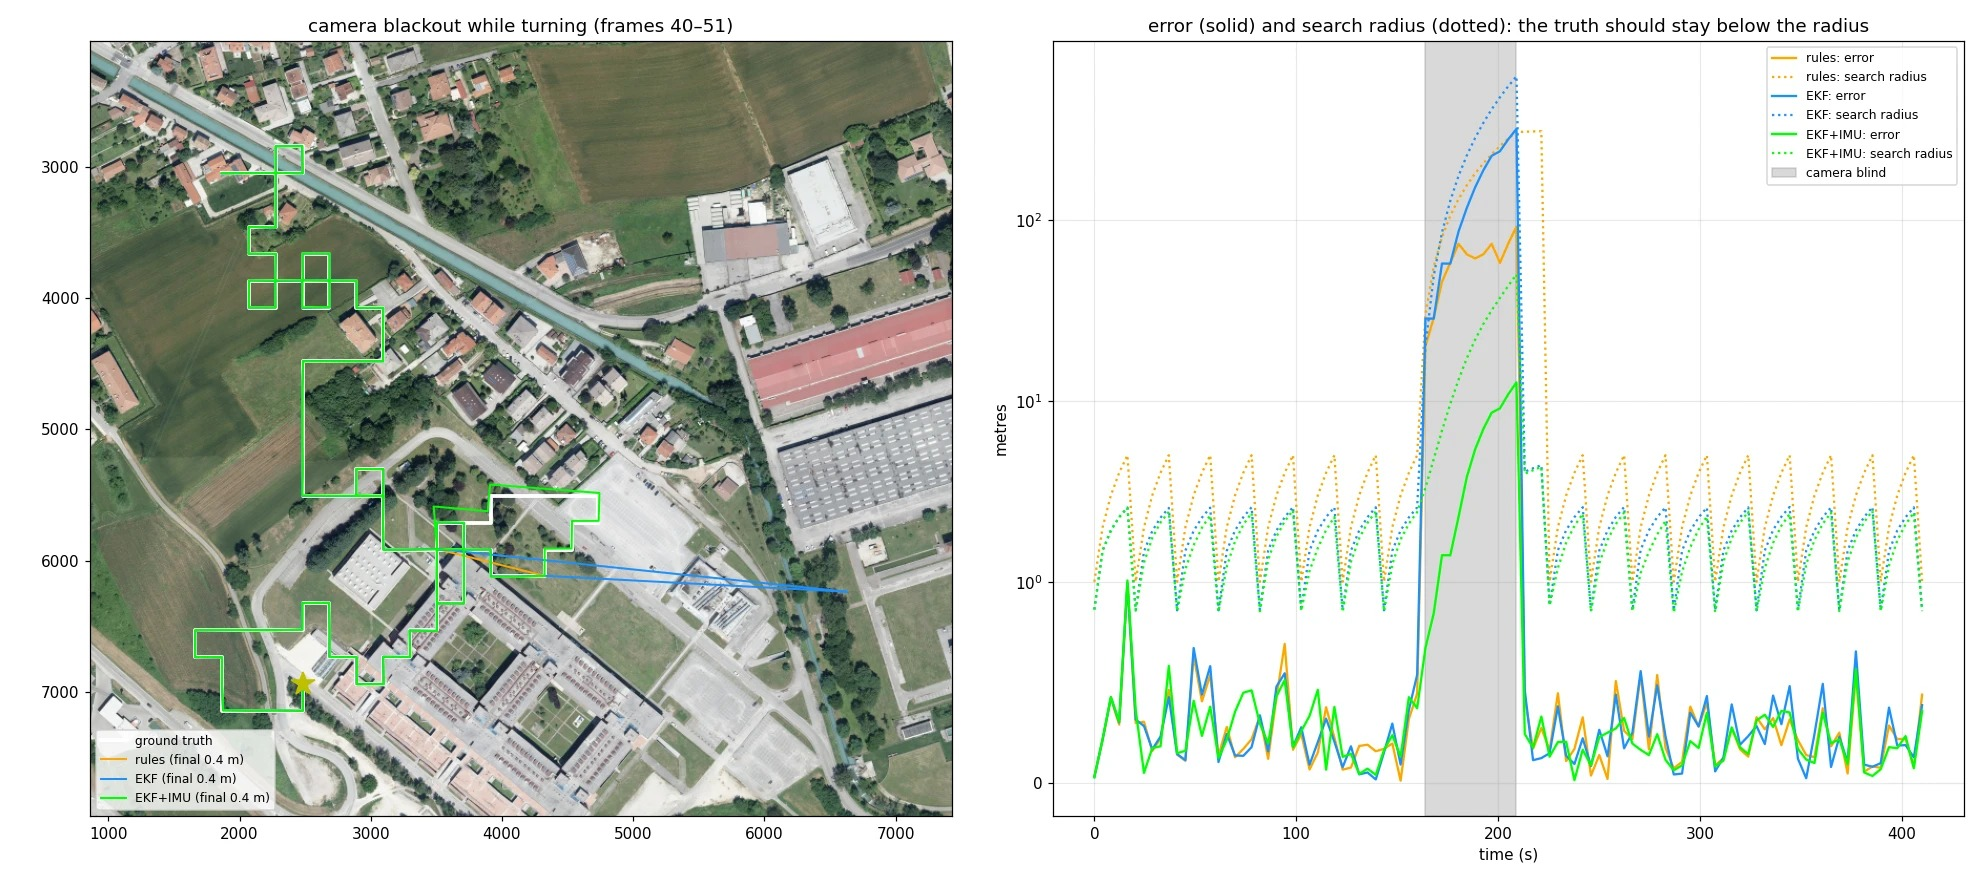
\includegraphics[width=\textwidth]{images/ekf-blackout-turning-seed26.jpg}
  \caption{Blackout while turning with the three modes}
  \label{fig:ekf-turn}
\end{figure}

The NEES values in the simulation (0.3--0.6, against an ideal of 2) show that the filter is too cautious there. It believes the error could be larger than it really is, because the simulated measurements are more accurate than the noise values assume. The one rejected fix in each scenario of the EKF without IMU (seed 101) led to an escalation and a successful relocalization.

On the real photos, flown as one flight without IMU, the results are those in Table~\ref{tab:ekf-real}. Note that the rules row differs slightly from Table~\ref{tab:reloc-all-real} (2.3~m against 2.0~m final error) because it comes from a separate run of the same pipeline: the map fixes and relocalizations are identical in both.

\begin{table}[!htbp]
  \centering
  \caption{The real photo flight with the rules and the EKF}
  \label{tab:ekf-real}
  \small
  \begin{tabular}{lrr}
    \toprule
    & Rules & EKF \\
    \midrule
    Final error (m) & 2.30 & 1.36 \\
    ATE (m) & 10.54 & 16.30 \\
    Max error (m) & 33.32 & 89.27 \\
    Within 5~m (\%) & 72.4 & 67.2 \\
    Truth in radius (\%) & 51.7 & 100.0 \\
    NEES mean & -- & 1.33 \\
    NEES in 95\% bound (\%) & -- & 98.3 \\
    Map fixes (accepted/attempted) & 10/15 & 7/7 \\
    Relocalizations (accepted/attempted) & 4/4 & 6/9 \\
    Escalations & 3 & 0 \\
    False fixes & 0 & 0 \\
    \bottomrule
  \end{tabular}
\end{table}

\begin{figure}[!htbp]
  \centering
  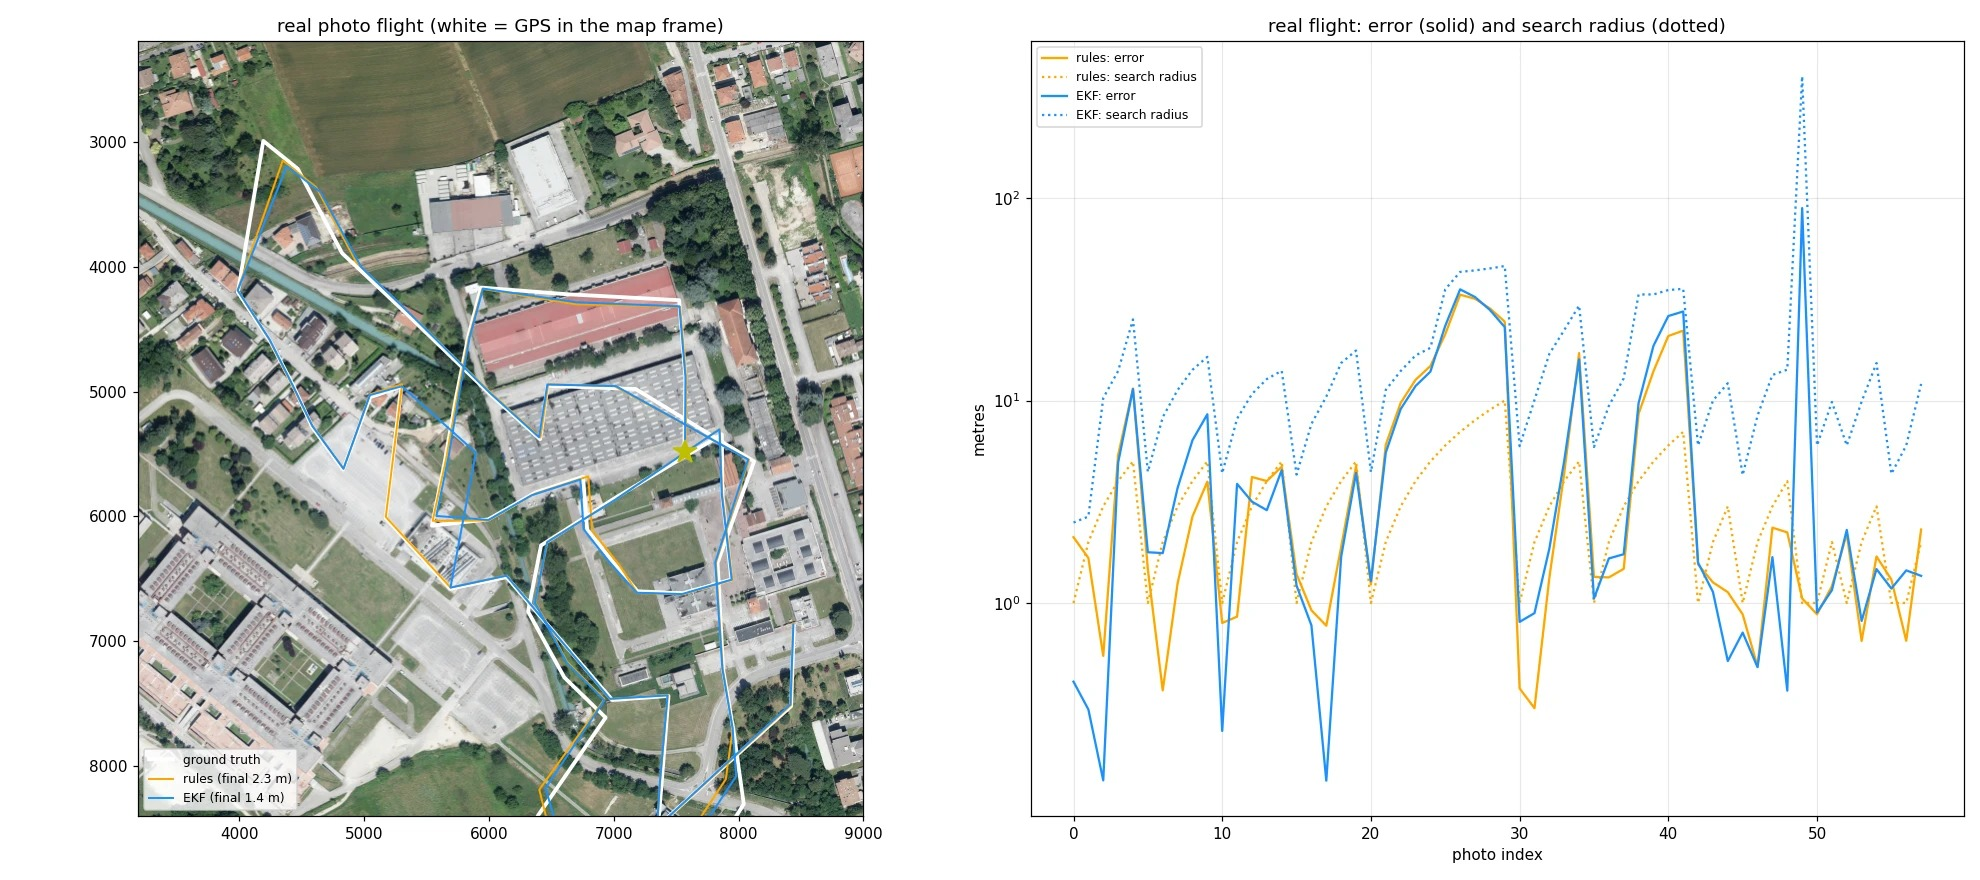
\includegraphics[width=\textwidth]{images/ekf-real-flight.jpg}
  \caption{The real photo flight with the rules and the EKF}
  \label{fig:ekf-real}
\end{figure}

The EKF ends closer to GPS (1.4~m against 2.3~m) and, most importantly, it knows how lost it is. The true position was inside its search radius on every photo, against 52\% for the rules, and its NEES of 1.33, with 98\% of photos within the 95\% bound, is consistent with the noise values chosen for the real photos. Its ATE is higher, 16.3~m against 10.5~m, and the per-photo log shows why. Photo 49 was taken 34~s and 106~m after the previous one. Constant-velocity prediction over 34~s placed the estimate 89~m off and grew the search radius to about 400~m. In that large area the retrieval did not find a verified place, so the drone was lost on that photo and recovered on the next one, 0.96~m from the GPS. The rules, by luck of their fixed increments, searched a smaller area and found it there. Without that single photo the two modes are equivalent: an ATE of 11.3~m against 10.6~m, with the same median error of 1.8~m.

Figure~\ref{fig:ekf-real} shows the real photo flight with the same two panels as Figure~\ref{fig:ekf-turn}. The EKF's search radius (dotted) stays above its error on every photo, while the radius of the rules repeatedly falls below their error. The single blue spike is the long gap at photo 49 discussed above.


The important takeaway here is that the EKF is useful both with and without the IMU data. With inertial data, the filter keeps the drone localized through camera blackouts (in simulation). Without it, the filter's main gain is a reliable estimate of its own uncertainty, which makes the decisions between map check and relocalization trustworthy. Without inertial data the filter does not improve the accuracy, and while the drone turns blind it is worse than the rules. The blackout results should also be read with one limit taken into account: the noise values of the filter were set on the same five simulated flights on which these results are reported.

\chapter{Evaluation on real flights}
\label{chap:evaluation}
Up until this point all of the tests and evaluations of the pipeline were performed on the same dataset, in which the real photos come from the same flight as the orthophoto: the camera and the map show the ground on the same day, in the same light and in the same season. This gives the pipeline an advantage when performing geo-localization, even with the augmentations applied to the data. The new dataset provided by Denis Tavaris from the University of Udine removes that advantage. The data was recorded on 28 October 2026 with a different drone, in a different season (autumn instead of spring) and about three and a half years after the flight of the first dataset (18 May 2023). Thus, even though the area of the flights is approximately the same, the pipeline is tested under the condition that matters most when evaluating how much it has overfitted to the first dataset: footage it has never seen before, including actual flight videos instead of simulated flights.

\section{Dataset and protocol}
\label{sec:real-protocol}
The given dataset holds two flights, named after the color of their path in the ground-truth files: orange and blue (Table~\ref{tab:real-flights}). Each of those flights has both still photos and one video. Both lie on tile 06611109, the same tile used in Chapters~\ref{chap:relocalization} and~\ref{chap:ekf}, so the same map and patch databases are used. A photo is $4000 \times 3000$~px with a focal length of 4.49~mm (24~mm in 35~mm equivalent), and the videos are $1920 \times 1080$~px at 29.97 frames per second. The drone stopped to take each photo and photographed most positions two or more times, so the photos are not a continuous flight. In Table~\ref{tab:real-flights}, photos taken within 5~m of each other count as one position.

\begin{table}[!htbp]
  \centering
  \caption{The two flights of the new dataset}
  \label{tab:real-flights}
  \small
  \begin{tabular}{lll}
    \toprule
     & Orange & Blue \\
    \midrule
    Role in the protocol & setup flight & held-out flight \\
    Photos & 24 & 25 \\
    Distinct positions & 9 & 13 \\
    Height above take-off & 59.9~m & 60.8~m \\
    Video & DJI\_0118 (114~s) & DJI\_0144 (91~s) \\
    Ground-truth path & 407~m & 287~m \\
    \bottomrule
  \end{tabular}
\end{table}

Since there were no IMU logs available from the flights, we ran the EKF without IMU data. The photos carry their GPS position as metadata, while the videos carry a subtitle track written once per second, with the GPS position rounded to four decimals (about 10~m), the distance from the home point, the height, the horizontal speed and a UTC time, as well as the attitude of the drone at the moment recording started. The stored heading of the drone is $-7.4^\circ$ for orange and $+6.4^\circ$ for blue, with the camera pointing straight down ($-89.9^\circ$). The ground truth is one KML path per flight, without timestamps, together with the home point. Thus, the reference position of a video frame had to be constructed: the time of the video is aligned with the distance along the KML path, by choosing for every second the point of the path at which the distance from home, the speed and the coarse GPS position of the subtitle agree best. A reference built this way is accurate across the path but uncertain by about $\pm 2$~m along it. For that reason the cross-track error, the distance of the estimate from the path, is reported next to the full error for every video flight.

The preparation of the data follows approximately the same pre-processing steps used for the first dataset (Section~\ref{sec:dataset}): the images are resized to the map resolution of 0.1~m per pixel, the scale is calibrated once at the start, and the offset between GPS and the map is measured leave-one-out (1.33~m west and 4.40~m south on orange, 1.62~m west and 2.71~m south on blue). The video frames need one additional factor of 1.17, because they show a narrower field of view than a photo. One problem of the calibration has to be noted. The blue flight starts directly above a house, and the start image was most likely matched on its roof, which is closer to the camera than the ground and therefore appears larger. The later map checks show that, as a result, the blue photos were processed about 15\% too small. This was found only after the blue runs and was not corrected, so that the blue flight stays held-out, which makes its results probably conservative.

The protocol used for the dataset was to set up the configuration on the orange flight and to run the blue flight once with it, as a held-out flight. Only what the new drone forces was set on orange: reading the heading and the focal length from the metadata, the video factor of 1.17, the number of start frames tried for the calibration, one video frame every 3~s as the main sequence, and padding the query with black rows when an image is lower than the 512~px patch. All other settings are the same as in Chapters~\ref{chap:vo} to~\ref{chap:ekf}. Four small departures from this protocol occurred:
\begin{itemize}
\item the blue flight was run before the orange results had been reviewed,
\item a first blue run stopped during the video stage and was repeated with the same settings,
\item the retriever comparison on blue was run again after the padding of the query was added,
\item both videos were run a second time with the start heading read from the video metadata, which on blue equals the heading measured in the first run.
\end{itemize}
No threshold or noise value was changed at any point.

The dataset was tested in three different cases:
\begin{enumerate}
\item Every image was treated separately, with a map check from 15~m off and then a search over the whole map. The same process was repeated for all three retrievers on both grids for the photos.
\item The photos and the video (one frame every 3~s, and also every 1, 6 and 10~s) of the new flights were flown through the whole pipeline, both with the rules and with the EKF (without IMU).
\item The video with one frame every 3~s was tested under an unknown start 254~m away and under a 15~s camera blackout at 40\% of the flight.
\end{enumerate}

\section{Results on single images}
\label{sec:real-single}
A correct fix is a verified position within 5~m of the reference, a false fix is one further away. Table~\ref{tab:real-single} gives the results with EfficientNet-B0 on the dense grid.

\begin{table}[!htbp]
  \centering
  \caption{Every image of the new flights treated alone}
  \label{tab:real-single}
  \footnotesize\setlength{\tabcolsep}{3.5pt}
  \begin{tabular}{lrrrrrrr}
    \toprule
     & & \multicolumn{2}{c}{Map check} & \multicolumn{4}{c}{Search from scratch} \\
    \cmidrule(lr){3-4}\cmidrule(lr){5-8}
     & & & Median & & & & Median \\
    Set & Images & Accepted & error (m) & R@5 & Correct & False & error (m) \\
    \midrule
    Orange photos, all & 24 & 15 & 0.53 & 0.88 & 15 & 0 & 0.50 \\
    Orange photos, one per position & 9 & 5 & 0.51 & 0.89 & 5 & 0 & 0.50 \\
    Orange video frames & 38 & 21 & 2.42 & 0.55 & 19 & 0 & 2.42 \\
    \addlinespace
    Blue photos, all & 25 & 23 & 0.48 & 0.60 & 22 & 0 & 0.34 \\
    Blue photos, one per position & 13 & 12 & 0.56 & 0.62 & 11 & 0 & 0.20 \\
    Blue video frames & 30 & 20 & 1.28 & 0.43 & 12 & 0 & 0.71 \\
    \bottomrule
  \end{tabular}
\end{table}

On the held-out blue flight the map check accepts 23 of the 25 photos at a median error of 0.48~m, and the search from scratch gives 22 correct fixes and no false fix. This is in the same range as on the photos of the first dataset (51 of 58 photos accepted by the map check at a median of 1.2~m, and 47 of 58 found from scratch), on imagery taken three and a half years after the map.

Within those 49 photos, the places that cannot be matched fall into two groups: vegetation (the canal, tree canopy and water, in autumn colors and with long morning shadows, where the map shows the same trees smaller and dark green) and a large roof that is now covered with solar panels, while it is nearly bare in the map. This means that the system has a hard time localizing itself wherever the ground no longer looks like the map, whether because of the season or because the ground itself has changed. On the orange flight this affected 9 of the 24 photos, all of them in its second photo session. On the blue flight it was only one position (two photos). Video frames are harder alone than photos: on blue the map check accepts 20 of 30 frames, but the search finds 12, with a Recall@5 of 0.43. A probable cause, which was not tested separately, is the size of the frame: after calibration a video frame is only 361~px high, so about 30\% of the 512~px query is black padding.

The comparison of the three retrievers (Chapter~\ref{chap:relocalization}) was repeated on the new photos, each searched from scratch. Table~\ref{tab:real-retrievers} gives the correct fixes out of the 24 orange and 25 blue photos and, in brackets, out of the 9 and 13 distinct positions. No retriever produced a false fix in 294 searches.

\begin{table}[!htbp]
  \centering
  \caption{The three retrievers on the new photos}
  \label{tab:real-retrievers}
  \small
  \begin{tabular}{llrrrr}
    \toprule
     & & \multicolumn{2}{c}{Orange} & \multicolumn{2}{c}{Blue} \\
    \cmidrule(lr){3-4}\cmidrule(lr){5-6}
    Retriever & Grid & Correct & R@5 & Correct & R@5 \\
    \midrule
    Autoencoder & 25.6~m & 6 (3) & 0.46 & 1 (1) & 0.00 \\
     & 6.4~m & 15 (5) & 0.88 & 14 (7) & 0.56 \\
    \addlinespace
    ResNet50 & 25.6~m & 13 (5) & 0.67 & 17 (9) & 0.48 \\
     & 6.4~m & 15 (5) & 0.63 & 16 (9) & 0.40 \\
    \addlinespace
    EfficientNet-B0 & 25.6~m & 11 (4) & 0.54 & 21 (11) & 0.48 \\
     & 6.4~m & 15 (5) & 0.88 & 22 (11) & 0.60 \\
    \bottomrule
  \end{tabular}
\end{table}

The comparison on the new dataset confirms the ranking of Chapter~\ref{chap:relocalization}: summed over both flights, EfficientNet-B0 gives the most correct fixes on both grids (37 on the dense grid and 32 on the coarse one, against 31 and 30 for ResNet50 and 29 and 7 for the autoencoder), while the autoencoder gives the fewest and nearly fails on the coarse grid (1 of 25 blue photos). The CNNs again depend much less on the dense grid than the autoencoder. Moving to the coarse grid, EfficientNet-B0 loses 1 photo on blue and 4 on orange, and ResNet50 gains 1 on blue and loses 2 on orange, while the autoencoder loses 13 and 9. The sample is small, however. On the orange flight all three retrievers find 15 of the 24 photos on the dense grid (not the same 15), and the 25 blue photos correspond to only 13 places, so the gap between ResNet50 and EfficientNet-B0 is only two places. What the data supports is that EfficientNet-B0 was equal or better on the dense grid of every dataset and in total on both grids, not that it is proven more accurate than ResNet50, which even found two more orange photos on the coarse grid.

\section{Results as flights}
\label{sec:real-flights}
In the same way as the simulated flights of the first dataset, the photos and the videos of the new flights were flown through the whole pipeline, with the rules and with the EKF. Errors are measured against the reference of each image, and the cross-track error, reported as a median, is the distance from the ground-truth path. No flight accepted a false fix. Table~\ref{tab:real-blue} gives the held-out blue flight and Table~\ref{tab:real-orange} the orange setup flight.

\begin{table}[!htbp]
  \centering
  \caption{The held-out blue flight}
  \label{tab:real-blue}
  \footnotesize\setlength{\tabcolsep}{2.4pt}
  \begin{tabular}{llrrrrrrrr}
    \toprule
     & & & ATE & Max & Final & Within & Truth in & & Cross- \\
    Flight & Mode & Frames & (m) & error (m) & error (m) & 5~m (\%) & radius (\%) & NEES & track (m) \\
    \midrule
    Photos & Rules & 25 & 1.46 & 5.97 & 1.48 & 96 & 96 & -- & -- \\
     & EKF & 25 & 2.02 & 5.73 & 1.57 & 96 & 100 & 0.97 & -- \\
    \addlinespace
    Video, 1~s & Rules & 90 & 2.46 & 5.91 & 3.50 & 98 & 84 & -- & 0.44 \\
     & EKF & 90 & 2.50 & 4.83 & 2.76 & 100 & 88 & 3.51 & 0.44 \\
    \addlinespace
    Video, 3~s & Rules & 30 & 3.09 & 5.19 & 4.25 & 93 & 80 & -- & 0.34 \\
     & EKF & 30 & 3.14 & 4.71 & 3.59 & 100 & 93 & 3.29 & 0.56 \\
    \addlinespace
    Video, 6~s & Rules & 15 & 5.01 & 11.64 & 5.00 & 80 & 47 & -- & 0.40 \\
     & EKF & 15 & 4.98 & 11.43 & 5.72 & 67 & 80 & 4.93 & 0.82 \\
    \addlinespace
    Video, 10~s & Rules & 9 & 7.98 & 12.31 & 6.45 & 44 & 22 & -- & 0.44 \\
     & EKF & 9 & 18.63 & 28.18 & 27.86 & 22 & 33 & 15.98 & 8.13 \\
    \addlinespace
    Unknown start & Rules & 30 & 2.53 & 4.70 & 2.05 & 100 & 77 & -- & 0.36 \\
     & EKF & 30 & 3.40 & 5.58 & 5.06 & 83 & 97 & 3.27 & 0.33 \\
    \addlinespace
    Blackout 15~s & Rules & 30 & 9.41 & 30.97 & 3.45 & 83 & 90 & -- & 0.63 \\
     & EKF & 30 & 9.82 & 41.81 & 2.20 & 87 & 97 & 2.08 & 1.05 \\
    \bottomrule
  \end{tabular}
\end{table}

\begin{table}[!htbp]
  \centering
  \caption{The orange setup flight}
  \label{tab:real-orange}
  \footnotesize\setlength{\tabcolsep}{3.5pt}
  \begin{tabular}{llrrrrrr}
    \toprule
     & & & ATE & Max & Final & Within & Truth in \\
    Flight & Mode & Frames & (m) & error (m) & error (m) & 5~m (\%) & radius (\%) \\
    \midrule
    Photos, session 0 & Rules & 9 & 0.34 & 0.55 & 0.35 & 100 & 100 \\
     & EKF & 9 & 0.42 & 0.57 & 0.57 & 100 & 100 \\
    \addlinespace
    Photos, session 1 & Rules & 15 & 3.59 & 6.47 & 6.47 & 93 & 87 \\
     & EKF & 15 & 4.31 & 7.44 & 7.44 & 60 & 100 \\
    \addlinespace
    Video, 1~s & Rules & 113 & 2.69 & 4.32 & 1.20 & 100 & 74 \\
     & EKF & 113 & 2.52 & 4.41 & 1.05 & 100 & 92 \\
    \addlinespace
    Video, 3~s & Rules & 38 & 2.84 & 4.49 & 0.90 & 100 & 79 \\
     & EKF & 38 & 2.85 & 4.43 & 1.07 & 100 & 97 \\
    \addlinespace
    Video, 6~s & Rules & 19 & 4.16 & 7.33 & 1.28 & 79 & 68 \\
     & EKF & 19 & 4.19 & 7.25 & 1.14 & 79 & 100 \\
    \addlinespace
    Video, 10~s & Rules & 12 & 35.54 & 81.53 & 2.61 & 67 & 67 \\
     & EKF & 12 & 21.94 & 57.37 & 2.51 & 75 & 100 \\
    \addlinespace
    Unknown start & Rules & 38 & 201.00 & 254.09 & 1.04 & 34 & 84 \\
     & EKF & 38 & 201.10 & 254.09 & 1.06 & 34 & 97 \\
    \addlinespace
    Blackout 15~s & Rules & 38 & 10.12 & 42.53 & 1.01 & 87 & 79 \\
     & EKF & 38 & 15.93 & 69.88 & 1.00 & 87 & 97 \\
    \bottomrule
  \end{tabular}
\end{table}

On blue, with one frame every 3~s, the 278~m video flight (the path between the sampled frames, against 287~m for the full ground-truth path, since the last frame is taken a few seconds before the video ends and corners are slightly cut) is followed with an ATE of 3.1~m in both modes (Figure~\ref{fig:real-blue-video}). Across the path the error is a median of 0.3--0.6~m and never above 3.6~m, so most of the full error lies along the path, where the reference itself is uncertain by about 2~m. The last map check, at frame 25, fails on ground that does not match the map, and the last nine frames run on odometry alone, ending about 4~m off. The 25 blue photos, whose reference is their own GPS position, give the cleanest numbers: an ATE of 1.5~m (rules) and 2.0~m (EKF), with 96\% of the photos within 5~m.

\begin{figure}[!htbp]
  \centering
  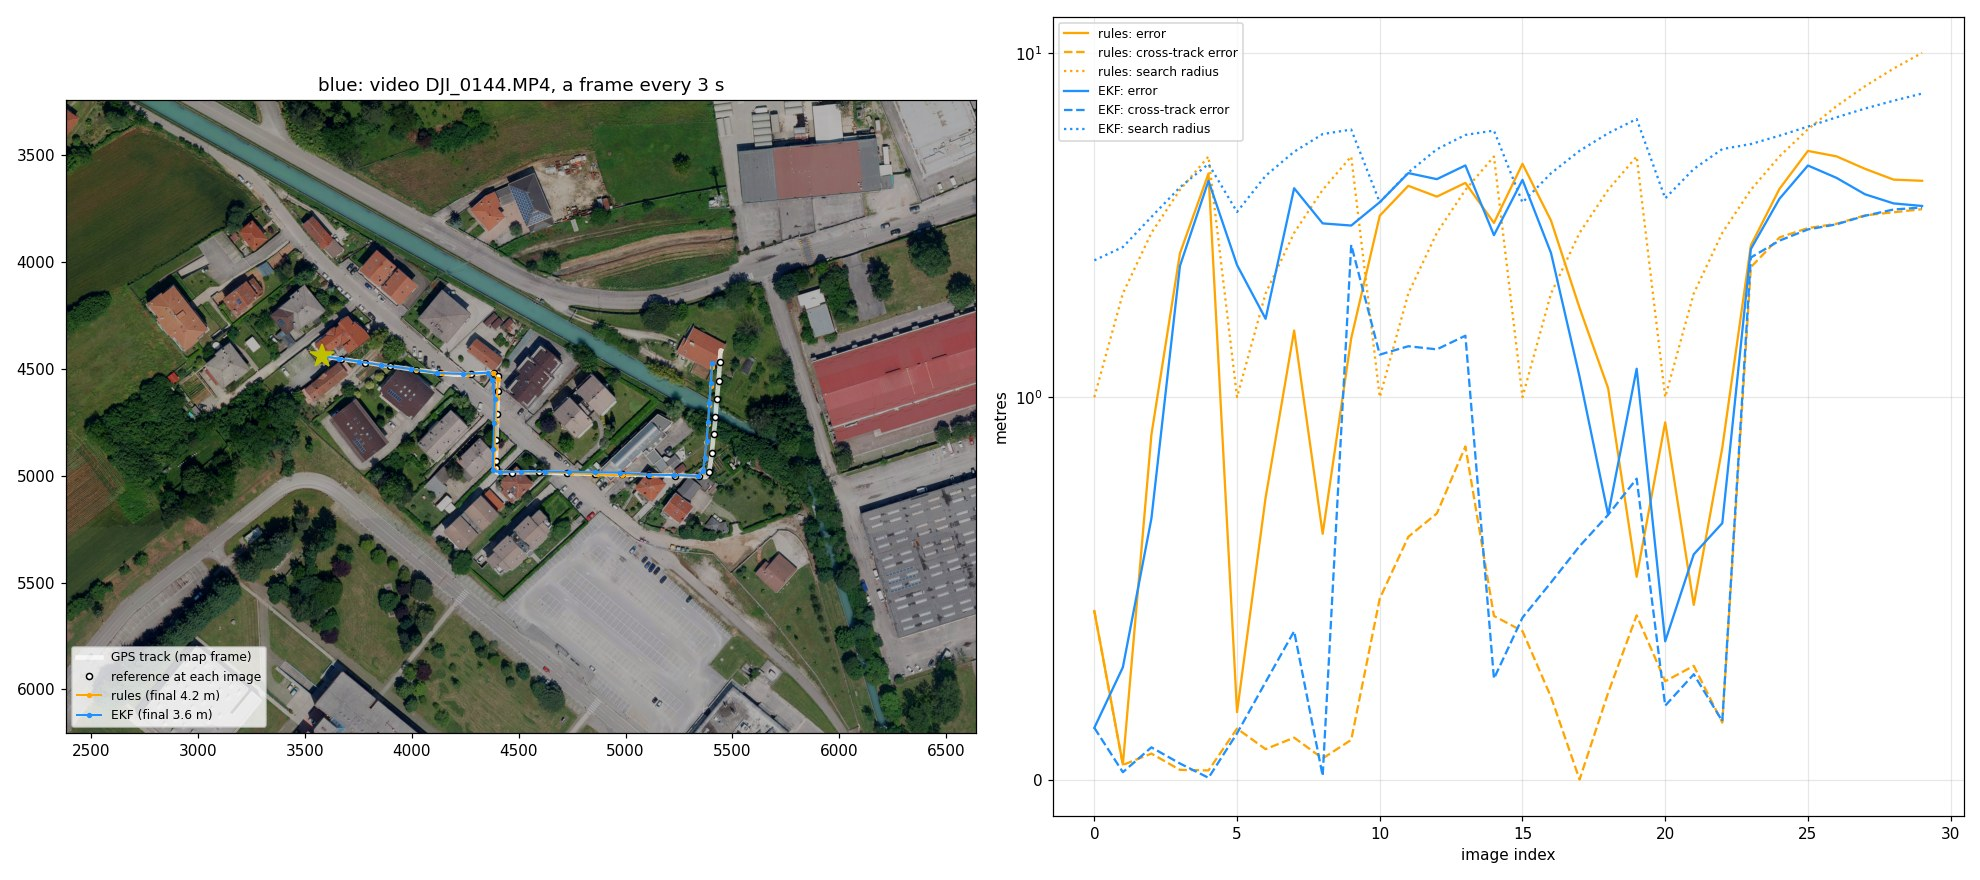
\includegraphics[width=\textwidth]{images/real-blue-video-flight.jpg}
  \caption{The held-out blue video flight, one frame every 3~s}
  \label{fig:real-blue-video}
\end{figure}

The EKF behaves as in Chapter~\ref{chap:ekf}: without an IMU it is not more accurate, but its uncertainty is more reliable, containing the true position on 80--93\% of the frames at 1--6~s spacing, against 47--84\% for the rules, whose growth of 1~m per step is too small on real video. On the video, however, its NEES is 3.3--4.9 instead of about 2, with only 60--83\% of the frames inside the 95\% bound, so it is overconfident with the noise values chosen on the photos of the first dataset. Part of this comes from the along-path uncertainty of the reference, which the filter does not know about. On the blue photos the NEES is 0.97.

Frame spacing shows how much overlap odometry needs. At 1~s and 3~s (90\% and 71\% overlap) the ATE is 2.5--3.1~m, at 6~s (40\%) it is 5.0~m, and at 10~s (19\%) it is 8.0~m with the rules and 18.6~m with the EKF, whose gate rejected the map check at frame 5. In an earlier run with the start heading measured from the map, the same map check was accepted and the ATE was 7.0~m. This case is decided by one measurement on nine frames, so the 10~s result is unstable rather than measured. Overall, the result supports the 80\% overlap chosen in simulation: accuracy degrades below about half overlap.

In the hard scenarios, an unknown start 254~m away is relocalized on the first blue image (0.4~m off), while the orange flight has nothing to match for its first 24 frames, stays about 250~m off and is within 4.2~m after its first relocalization at frame 25. In the 15~s blackout (59--64~m flown blind) the error peaks at 31.0~m (rules) and 41.8~m (EKF) on blue (Figure~\ref{fig:real-blue-blackout}) and at 42.5~m and 69.9~m on orange, as the constant-velocity prediction of the EKF overshoots, and it is back to about 1~m on the first frame after the blackout. This is the real-data counterpart of the simulated blackout without IMU. The 3.9~m of Chapter~\ref{chap:ekf} has no counterpart here, because no inertial data exists for these flights.

\begin{figure}[!htbp]
  \centering
  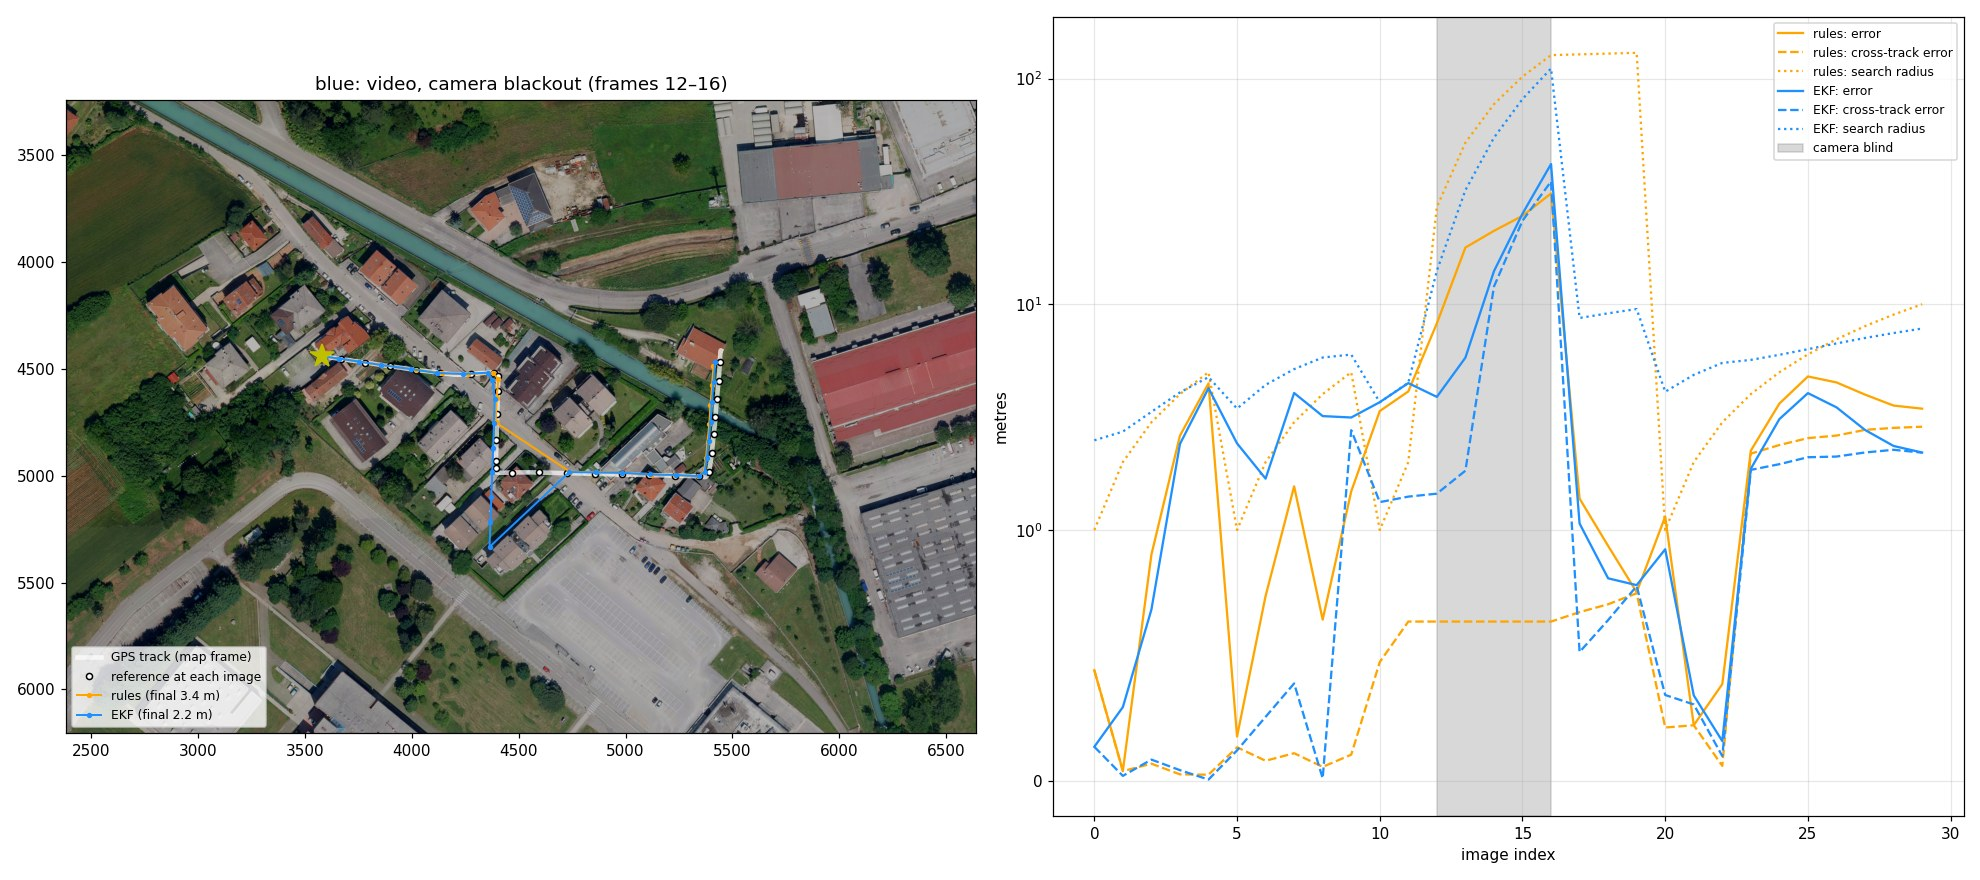
\includegraphics[width=\textwidth]{images/real-blue-blackout.jpg}
  \caption{The blue video flight with a camera blackout of 15~s (frames 12--16)}
  \label{fig:real-blue-blackout}
\end{figure}

The orange video starts over ground that rarely matches the map: only 5 of its first 18 frames pass the map check alone, against 16 of the last 20. Its start frame could therefore not be used for the calibration, and the flight runs with the nominal scale and the heading stored in the video. With these two values it is followed within 4.5~m at 3~s spacing. An earlier run that assumed a heading of $0^\circ$ instead drifted to 27.6~m, which is what a heading error of $7.4^\circ$ produces over about 215~m of flight. This shows how much the pipeline depends on the start heading when the start cannot be matched to the map.

\section{Runtime on the Jetson Orin Nano}
\label{sec:jetson-runtime}
The next logical step is to see whether the pipeline is capable of running in real time on hardware that could be attached to a drone. For that reason, the flights of the previous section were run, with unchanged code and settings, on a Jetson Orin Nano Super provided by Denis Tavaris from the University of Udine (8~GB of memory shared by the CPU and the GPU, MAXN SUPER power mode, JetPack 6.2.1, PyTorch 2.11 \citep{paszke2019pytorch}). The pipeline was run twice on the blue flight and once on the orange flight, and the three retrievers were then timed in a separate script. Each stage was timed 30 times after 3 warm-up runs, every frame was also timed during the flights, and the memory, power and temperature of the board were logged once per second. Reading the images from disk is not included. Table~\ref{tab:jetson-stages} and Figure~\ref{fig:jetson-stages} give the time of each stage, as the median of 30 runs on the second blue run. The other two runs agree within 1--2\%.

\begin{table}[!htbp]
  \centering
  \caption{Time per stage on the Jetson Orin Nano Super}
  \label{tab:jetson-stages}
  \small
  \begin{tabular}{lr}
    \toprule
    Stage & Median (ms) \\
    \midrule
    SuperPoint, one camera image & 83 \\
    SuperPoint, one 1024~px map crop & 154 \\
    LightGlue, two images & 65 \\
    RANSAC motion estimate (CPU) & 0.4 \\
    Odometry step & 246 \\
    Map check & 362 \\
    Fingerprint, EfficientNet-B0 & 27 \\
    Search of the dense database (CPU) & 4.7 \\
    Relocalization over the whole map, 5 candidates & 1700 \\
    EKF, one image (CPU) & 0.32 \\
    \bottomrule
  \end{tabular}
\end{table}

\begin{figure}[!htbp]
  \centering
  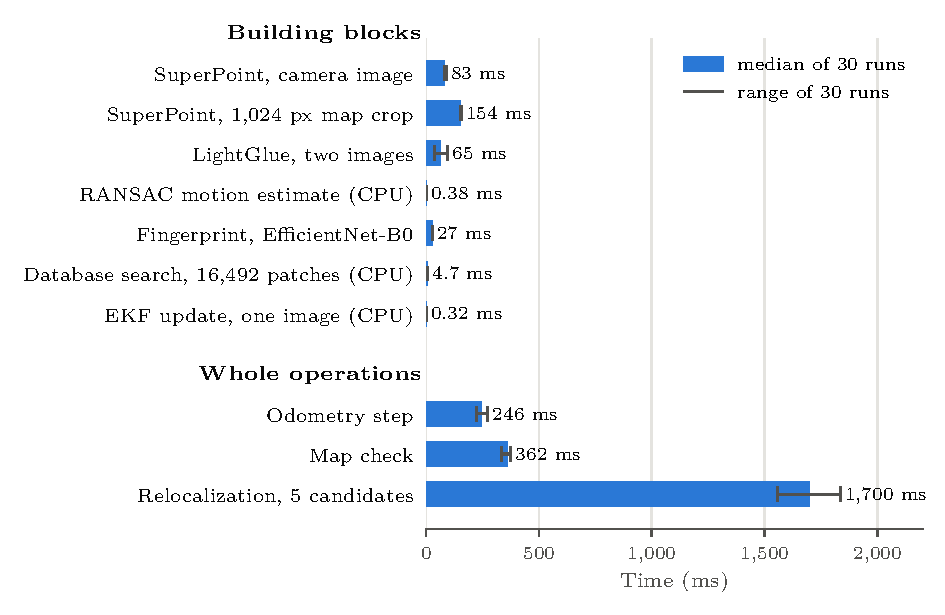
\includegraphics[width=0.85\textwidth]{images/jetson-stage-times.pdf}
  \caption{Time per stage on the Jetson Orin Nano Super}
  \label{fig:jetson-stages}
\end{figure}

SuperPoint and LightGlue make up about 94\% of an odometry step, and the fingerprint and the search together are under 2\% of a relocalization. LightGlue is the only stage whose time varies (39--95~ms), because it depends on the number of keypoints. Figure~\ref{fig:jetson-stages} shows the median and the range of the 30 runs of each stage. In flight a normal frame takes about 0.25~s (median per flight 248--325~ms), and the time of a frame depends on what happens in it (Table~\ref{tab:jetson-frames}).

\begin{table}[!htbp]
  \centering
  \caption{Time per frame in flight by what happened in the frame}
  \label{tab:jetson-frames}
  \small
  \begin{tabular}{lrr}
    \toprule
     & Blue: median & Orange: median \\
    What happened in the frame & ms (frames) & ms (frames) \\
    \midrule
    Odometry only & 270 (86) & 272 (96) \\
    Odometry and an accepted map check & 630 (16) & 603 (12) \\
    Odometry and a failed map check & 637 (5) & 2224 (8) \\
    Relocalization & 2230--2445 (3) & 1967--2324 (4) \\
    Lost (all three failed) & -- & 3885 (4) \\
    \bottomrule
  \end{tabular}
\end{table}

At one image every 3~s, every blue frame finishes before the next image arrives. On orange, 3 of 38 video frames take longer (up to 4.1~s), all of them frames in which the drone is lost and searches again. At one image per second, odometry and map-check frames would still fit, but a relocalization (about 2~s) would not.

Table~\ref{tab:jetson-retrievers} gives the median time of one $512 \times 512$ query for each retriever (30 runs on the GPU, 10 on the CPU), its GPU memory and its size. The autoencoder and ResNet50 ran with random weights, which is valid for time and memory, since both depend on the shape of a network and not on its weights. EfficientNet-B0 is slow on the ARM CPU because of how PyTorch handles its depthwise convolutions. This does not affect the GPU.

\begin{table}[!htbp]
  \centering
  \caption{The three retrievers on the Jetson Orin Nano Super}
  \label{tab:jetson-retrievers}
  \footnotesize\setlength{\tabcolsep}{4pt}
  \begin{tabular}{lrrrrrr}
    \toprule
     & GPU & CPU & GPU memory & Parameters & Fingerprint & Database \\
    Retriever & (ms) & (ms) & (MB) & (M) & length & (MB) \\
    \midrule
    Autoencoder & 149.7 & 2215 & 1081 & 268.8 & 2048 & 128.8 \\
    ResNet50 & 29.7 & 254 & 121 & 23.5 & 2048 & 128.8 \\
    EfficientNet-B0 & 26.2 & 1767 & 35 & 4.0 & 1280 & 80.5 \\
    \bottomrule
  \end{tabular}
\end{table}

EfficientNet-B0 is the fastest network on the GPU, while the autoencoder needs 1.08~GB of GPU memory, thirty times more, which on a board with 7.4~GB shared between CPU and GPU is the strongest practical argument against it. The whole pipeline uses 0.7~GB of GPU memory and 2.8~GB for the whole process (the board never exceeded 5.2~GB), draws 15.7--17.0~W on average (19.1~W at most) and stayed below 70~$^\circ$C. The fingerprint database takes 81~s to build, once per map, and occupies 80.5~MB.

The two blue runs gave identical positions, so the pipeline is deterministic on the board. Compared with the runs on Colab, the accepted photo map checks differ by a median of 0.06~m, and most flights agree within about 0.5~m of ATE. The one large difference is the blue video with the EKF: on the Jetson the map check at frame 10 lands slightly further from the prediction, the $\chi^2$ gate rejects it, and the ATE grows from 3.1 to 5.5~m. The cause is that the GPU of the Jetson rounds the arithmetic of SuperPoint and LightGlue slightly differently and that a different OpenCV version draws the random samples of RANSAC differently. Near the threshold of the gate, such small differences can flip its decision. For that reason, the accuracy results of this thesis are those obtained on Colab, and the times are those of the Jetson. The times are an upper bound: the board ran plain PyTorch with 32-bit numbers, without TensorRT or 16-bit precision, with clocks that were not fixed, in the lab on wall power.

\section{Discussion}
\label{sec:real-discussion}
To sum up, the pipeline proved that it transfers to new footage without retraining or retuning. On the held-out (blue) flight a map check locates a photo to about 0.5~m, a photo is found from scratch in 22 of 25 cases, and a 278~m video flight (one frame every 3~s) is followed with an ATE of about 3~m, part of which is the uncertainty of the reference. EfficientNet-B0 is the best retriever and the autoencoder the weakest, the CNNs work on the coarse grid, LightGlue verification never accepted a wrong place, and the EKF without IMU improves the reliability of the uncertainty, not the accuracy. All of this corresponds to what we concluded in Chapters~\ref{chap:relocalization} and~\ref{chap:ekf} from the simulated flights and the photos of the first dataset, and the pipeline runs in real time on the Jetson Orin Nano at one image every 3~s.

The new flights also show the limits of the system. It depends on the map still matching the ground. Where it does, the error is below a meter. Where it does not, as on the first half of the orange video, the drone has only odometry. The scale calibration on a single start image is the weak point on both flights, since it failed on orange and was biased by a roof on blue. Calibrating from several map checks along the first part of the flight would remove it. Finally, the evidence is two short flights on one tile, with 13 distinct positions on the held-out flight, the reference is a corrected GPS position and a time-aligned path rather than a surveyed truth, and without IMU recordings the result of the EKF with inertial data from Chapter~\ref{chap:ekf} could not be tested on real flights.

\chapter{Conclusions}
\label{chap:conclusions}
This chapter summarizes what has been done within the scope of this project, including the limitations of the developed pipeline and the gaps to be addressed in the future.

\section{Main findings}
\label{sec:findings}
The main question this thesis was trying to answer was whether a drone without GPS can accurately locate itself from a downward-looking camera and an on-board orthophoto, even when the drone has lost track of its position. The short answer is yes. Both in the simulations on the first dataset and on the actual flights in the second one, the pipeline achieved high-precision drone geo-localization within the outlined constraints. Overall, this project had the following results:

\begin{itemize}
\item \textbf{Odometry} (Chapter~\ref{chap:vo}). Frame-to-frame odometry with SuperPoint + LightGlue is accurate enough to navigate on. Over 240 simulated flights on six tiles, it drifts by a median of 0.64~m over 512~m, about one part in 800, against 82~m for EfficientLoFTR. About 74\% of LightGlue's matches agree with one motion, against 2\% for EfficientLoFTR, and the known-answer tests and the ablation show that rotation and photometric change each break EfficientLoFTR on their own. The remaining error of the odometry comes from image quality, not from the geometry of the model.

\item \textbf{Map check} (Chapters~\ref{chap:vo}--\ref{chap:relocalization}). Matching the camera image against the map at the estimated position removes the drift. In simulation, the drone ends 0.18~m from the truth after 2~km. On Fabris's real photos, the map check locates 51 of 58 with a median error of 1.2~m.

\item \textbf{Relocalization} (Chapter~\ref{chap:relocalization}). Retrieval followed by LightGlue verification recovers a lost drone. Every simulated blackout and wrong start was recovered, and no wrong position was accepted in any flight, with any retriever, in simulation or on real data. The retrieval step only proposes candidates. The position itself always comes from the LightGlue verification.

\item \textbf{The autoencoder} (Chapter~\ref{chap:relocalization}). Since this work builds on Fabris's autoencoder, it was tested in the same pipeline as the CNNs. Fabris's autoencoder recognizes a place only within about 3~m of a patch center. This explains why its accuracy falls from 71\% on his test crops (median 1.4~m from a patch center) to about 5\% on real photos (median 10.8~m), and why it needs the dense 6.4~m grid to work at all. On every real-data test it was clearly outperformed by the pretrained CNNs.

\item \textbf{Pretrained CNNs} (Chapter~\ref{chap:relocalization}). ResNet50 and EfficientNet-B0, neither of which saw this map or was fine-tuned on it, do the retrieval job better. On the dense grid they find 47 of the 51 findable real photos against 28 for the autoencoder, and the real photo flight ends about 2~m from GPS instead of 195~m. They also barely need the dense grid (44 against 11 photos on Fabris's grid). EfficientNet-B0 is equal to or better than the alternatives and much lighter, with 4 million parameters against 23.5 million for ResNet50 and 269 million for the autoencoder.

\item \textbf{Rules and EKF} (Chapter~\ref{chap:ekf}). The EKF makes the drone's uncertainty reliable. On the real photos the true position is inside its search radius on every photo, against 52\% with the fixed rules. With simulated inertial data it keeps the drone within a median maximum error of 3.9~m through a 12-frame (about 50~s) camera blackout on a straight leg, where the rules drift 246~m, and within 5.8~m when the drone keeps turning (rules 92~m). Without inertial data it does not improve accuracy and is worse than the rules while turning, because constant-velocity prediction carries the estimate straight on.

\item \textbf{Real flights} (Chapter~\ref{chap:evaluation}). The system transfers to footage it has never seen. The held-out flight was recorded three and a half years after the map, in another season and with a different drone, and no setting was changed. On it, a map check locates a photo to about 0.5~m, 22 of 25 photos are found from scratch with EfficientNet-B0 (14 with the autoencoder), and a 278~m video flight (one frame every 3~s) is followed with an ATE of about 3~m, most of it along the path where the reference itself is uncertain. The ranking of the retrievers and the behavior of the EKF are the same as in Chapters~\ref{chap:relocalization} and~\ref{chap:ekf}.

\item \textbf{On-board runtime} (Chapter~\ref{chap:evaluation}). The pipeline runs in real time on a Jetson Orin Nano Super at one image every 3~s: an odometry step takes 0.25~s, a map check 0.36~s and a relocalization 1.7~s, with 0.7~GB of GPU memory and about 16--17~W. SuperPoint and LightGlue take about 94\% of the time, while EfficientNet-B0 needs 26~ms and 35~MB of GPU memory per fingerprint, against 150~ms and 1081~MB for the autoencoder. The autoencoder's memory use is the strongest practical argument against using it on the drone.
\end{itemize}

In relation to the literature reviewed in Chapter~\ref{chap:background}, the pipeline follows the established coarse-to-fine scheme of hierarchical localization \citep{sarlin2019hloc}: candidates are retrieved with a global descriptor and verified with local features. The contribution of this thesis is therefore not a new architecture. It is a controlled comparison of matchers, retrievers and fusion methods on the same data with known-answer tests, a diagnosis of the autoencoder's behavior in conditions different from those it was trained for, and evidence that real-time geo-localization of a UAV based on computer vision is already possible and runs in real time on a board of the kind a drone carries.

\clearpage% keep the whole section on one page
\section{Limitations}
\label{sec:limitations}
Like any other system of this kind, the pipeline has gaps and limitations that should be noted:

\begin{itemize}
\item The odometry benchmark covers six tiles, but everything after it (the retriever comparison, the EKF and both real datasets) uses tile 06611109 only. The retrievers have never been tested on a second map, so the ranking of Chapter~\ref{chap:relocalization} is shown for one area of about $900 \times 840$~m. The real data is also small: 58 photos from one flight and two short new flights, with 13 distinct positions on the held-out one. That is enough to show the differences between the methods, but not to give precise success rates: on 25 photos, one photo more or less changes a rate by 4 points. Finally, the real-flight errors are measured against the drone's consumer GPS, which is itself off by a few meters, so part of the reported error belongs to the reference rather than to the pipeline.

\item No real inertial data exists for any flight. The simulated IMU is two-dimensional and follows the filter's own noise model, and in simulation the camera image and the map come from the same orthophoto on the same pixel grid, differing only in color. Simulated numbers such as 0.18~m after 2~km or 3.9~m through a blackout therefore show that the method works as designed and are upper bounds on what a real flight would give. On the real video, where only the filter without IMU could be tested, a 15~s blackout gives a peak error of 31 to 70~m. The blackout baseline is also weak: the rules hold their last position while the drone flies on, so any method that keeps moving beats them. Rotation, finally, is tested mainly in simulation, since Fabris's photos are north-up within about $2^\circ$ and the new flights stay within about $\pm 10^\circ$.

\item The thresholds of the pipeline (the 50-inlier gate, the 30~m and 60~m limits, a map check every 5 images) and the noise values of the EKF were chosen while looking at the same simulations and photos on which they are reported. The simulated IMU noise and heading term were likewise set on the same five seeds as the blackout results. None was tuned aggressively, and the gate sweep shows the main threshold is not sensitive. The held-out blue flight partly answers this for the real data: the pipeline transferred unchanged, but the EKF was overconfident on the new video (NEES 3.3 to 4.9 instead of about 2), partly because of the uncertain reference. The simulated results still have no held-out seeds.

\item On the new flights every place that could not be matched was ground that had changed since the map: vegetation in another season and a roof now covered with solar panels. There the drone has only odometry. The start calibration from a single image is the weakest step: it failed on the orange video and was biased by a roof on the blue flight, and the flat-ground model is strained at about 55~m over houses.

\item The $\chi^2$ gate is applied only to map checks and relocalizations, so a wrong odometry step is limited only by the inlier and scale rules. Fabris's method is scored against a 5~m threshold that it cannot meet by construction, since it outputs patch centers on a 25.6~m grid, and the autoencoder is used here on a dense grid and inside a pipeline it was not designed for.
\end{itemize}

\clearpage% keep the whole section on one page
\section{Future work}
\label{sec:future-work}
Directly following the limitations mentioned above, the following points are proposed as future improvements of the pipeline:

\begin{itemize}
\item The retriever comparison and the full pipeline should be tested on another tile or, better, another area. That would show whether the ranking of Chapter~\ref{chap:relocalization} holds beyond one map.
\item A flight with the inertial data recorded would replace the simulated IMU, and it is the only way to confirm the blackout result of Chapter~\ref{chap:ekf} on real data.
\item GPS should be settled against the map with an independent reference, for example surveyed ground points, and the EKF should be calibrated on held-out data, including new simulation seeds.
\item The thesis uses a high-resolution aerial orthophoto. Satellite imagery is coarser, older and covers far larger areas, which would test both the matcher and the retrieval at a much larger scale. This is also where the title's mention of satellite maps belongs.
\item Fine-tuning was deliberately left out, so that the comparison isolates the effect of the pretrained network. Fine-tuning the CNN on aerial imagery is the first step. Foundation-model features such as DINOv2 \citep{oquab2023dinov2}, used without fine-tuning as in AnyLoc \citep{keetha2023anyloc} or with a small adapter as in \citet{li2024crossview}, are the natural next retriever, following the same idea as this thesis with a stronger network.
\item The start could be made more robust by calibrating the scale from several map checks along the first part of the flight instead of a single image. Features less sensitive to season, or an updated map, would reduce the places where the drone cannot match the ground.
\item The Jetson measurement was done in the lab, so the next step is an optimized version (TensorRT, 16-bit numbers) with the camera capture time included, and a test with the board on the flying drone.
\end{itemize}

\backmatter
\phantomsection
\begin{thebibliography}{99}

\bibitem[Amer et~al.(2017)]{amer2017urban}
Amer, K., Samy, M., ElHakim, R., Shaker, M., \& ElHelw, M. (2017).
Convolutional neural network-based deep urban signatures with application to drone localization.
In \textit{Proceedings of the IEEE International Conference on Computer Vision Workshops} (pp.~2138--2145). \url{https://openaccess.thecvf.com/content_ICCV_2017_workshops/w30/html/Amer_Convolutional_Neural_Network-Based_ICCV_2017_paper.html}

\bibitem[Arandjelovi{\'c} et~al.(2016)]{arandjelovic2016netvlad}
Arandjelovi{\'c}, R., Gronat, P., Torii, A., Pajdla, T., \& Sivic, J. (2016).
NetVLAD: CNN architecture for weakly supervised place recognition.
In \textit{Proceedings of the IEEE Conference on Computer Vision and Pattern Recognition} (pp.~5297--5307). \url{https://doi.org/10.1109/CVPR.2016.572}

\bibitem[Bar-Shalom et~al.(2001)]{barshalom2001}
Bar-Shalom, Y., Li, X.~R., \& Kirubarajan, T. (2001).
\textit{Estimation with applications to tracking and navigation: Theory, algorithms and software}.
Wiley. \url{https://doi.org/10.1002/0471221279}

\bibitem[Bradski(2000)]{bradski2000opencv}
Bradski, G. (2000).
The OpenCV library.
\textit{Dr. Dobb's Journal of Software Tools}.

\bibitem[Buslaev et~al.(2020)]{buslaev2020albumentations}
Buslaev, A., Iglovikov, V.~I., Khvedchenya, E., Parinov, A., Druzhinin, M., \& Kalinin, A.~A. (2020).
Albumentations: Fast and flexible image augmentations.
\textit{Information}, \textit{11}(2), 125. \url{https://doi.org/10.3390/info11020125}

\bibitem[Cabrera-Ponce \& Martinez-Carranza(2022)]{cabrera2022geoloc}
Cabrera-Ponce, A.~A., \& Martinez-Carranza, J. (2022).
Convolutional neural networks for geo-localisation with a single aerial image.
\textit{Journal of Real-Time Image Processing}, \textit{19}, 565--575. \url{https://doi.org/10.1007/s11554-022-01207-1}

\bibitem[Couturier \& Akhloufi(2024)]{couturier2024avl}
Couturier, A., \& Akhloufi, M.~A. (2024).
A review on deep learning for UAV absolute visual localization.
\textit{Drones}, \textit{8}(11), 622. \url{https://doi.org/10.3390/drones8110622}

\bibitem[Deng et~al.(2009)]{deng2009imagenet}
Deng, J., Dong, W., Socher, R., Li, L.-J., Li, K., \& Fei-Fei, L. (2009).
ImageNet: A large-scale hierarchical image database.
In \textit{Proceedings of the IEEE Conference on Computer Vision and Pattern Recognition} (pp.~248--255). \url{https://doi.org/10.1109/CVPR.2009.5206848}

\bibitem[DeTone et~al.(2018)]{detone2018superpoint}
DeTone, D., Malisiewicz, T., \& Rabinovich, A. (2018).
SuperPoint: Self-supervised interest point detection and description.
In \textit{Proceedings of the IEEE Conference on Computer Vision and Pattern Recognition Workshops} (pp.~224--236). \url{https://arxiv.org/abs/1712.07629}

\bibitem[DJI(2016)]{dji2016phantom4}
DJI. (2016).
\textit{Phantom 4 user manual} (Version 1.0).
SZ DJI Technology Co., Ltd. \url{https://dl.djicdn.com/downloads/phantom_4/en/Phantom_4_User_Manual_en_v1.0.pdf}

\bibitem[Durgam et~al.(2024)]{durgam2024crossview}
Durgam, A., Paheding, S., Dhiman, V., \& Devabhaktuni, V. (2024).
Cross-view geo-localization: A survey.
\textit{IEEE Access}, \textit{12}. \url{https://doi.org/10.1109/ACCESS.2024.3507280}

\bibitem[Fabris(2025)]{fabris2025thesis}
Fabris, A. (2025).
\textit{Real-time localization algorithm for GPS-denied drone navigation} [Unpublished master's thesis].
University of Udine.

\bibitem[Fischler \& Bolles(1981)]{fischler1981ransac}
Fischler, M.~A., \& Bolles, R.~C. (1981).
Random sample consensus: A paradigm for model fitting with applications to image analysis and automated cartography.
\textit{Communications of the ACM}, \textit{24}(6), 381--395. \url{https://doi.org/10.1145/358669.358692}

\bibitem[He et~al.(2016)]{he2016resnet}
He, K., Zhang, X., Ren, S., \& Sun, J. (2016).
Deep residual learning for image recognition.
In \textit{Proceedings of the IEEE Conference on Computer Vision and Pattern Recognition} (pp.~770--778). \url{https://doi.org/10.1109/CVPR.2016.90}

\bibitem[InvenSense(2015)]{invensense2015mpu6500}
InvenSense. (2015).
\textit{MPU-6500 product specification}.
InvenSense Inc. \url{https://www.mouser.com/datasheet/2/400/MPU-6500-Datasheet2-1112506.pdf}

\bibitem[Kalman(1960)]{kalman1960}
Kalman, R.~E. (1960).
A new approach to linear filtering and prediction problems.
\textit{Journal of Basic Engineering}, \textit{82}(1), 35--45. \url{https://doi.org/10.1115/1.3662552}

\bibitem[Keetha et~al.(2023)]{keetha2023anyloc}
Keetha, N., Mishra, A., Karhade, J., Jatavallabhula, K.~M., Scherer, S., Krishna, M., \& Garg, S. (2023).
AnyLoc: Towards universal visual place recognition.
arXiv. \url{https://arxiv.org/abs/2308.00688}

\bibitem[Kerns et~al.(2014)]{kerns2014spoofing}
Kerns, A.~J., Shepard, D.~P., Bhatti, J.~A., \& Humphreys, T.~E. (2014).
Unmanned aircraft capture and control via GPS spoofing.
\textit{Journal of Field Robotics}, \textit{31}(4), 617--636. \url{https://doi.org/10.1002/rob.21513}

\bibitem[Khan et~al.(2021)]{khan2021spoofing}
Khan, S.~Z., Mohsin, M., \& Iqbal, W. (2021).
On GPS spoofing of aerial platforms: A review of threats, challenges, methodologies, and future research directions.
\textit{PeerJ Computer Science}, \textit{7}, e507. \url{https://doi.org/10.7717/peerj-cs.507}

\bibitem[Li et~al.(2024)]{li2024crossview}
Li, H., Xu, C., Yang, W., Yu, H., \& Xia, G.-S. (2024).
Learning cross-view visual geo-localization without ground truth.
arXiv. \url{https://arxiv.org/abs/2403.12702}

\bibitem[M.~Lin et~al.(2014)]{lin2014nin}
Lin, M., Chen, Q., \& Yan, S. (2014).
Network in network.
In \textit{International Conference on Learning Representations}. \url{https://arxiv.org/abs/1312.4400}

\bibitem[T.-Y.~Lin et~al.(2014)]{lin2014coco}
Lin, T.-Y., Maire, M., Belongie, S., Hays, J., Perona, P., Ramanan, D., Doll{\'a}r, P., \& Zitnick, C.~L. (2014).
Microsoft COCO: Common objects in context.
In \textit{Computer Vision -- ECCV 2014} (pp.~740--755). Springer. \url{https://doi.org/10.1007/978-3-319-10602-1_48}

\bibitem[Lindenberger et~al.(2023)]{lindenberger2023lightglue}
Lindenberger, P., Sarlin, P.-E., \& Pollefeys, M. (2023).
LightGlue: Local feature matching at light speed.
In \textit{Proceedings of the IEEE/CVF International Conference on Computer Vision} (pp.~17627--17638). \url{https://arxiv.org/abs/2306.13643}

\bibitem[Liu et~al.(2025)]{liu2025survey}
Liu, H., Long, Q., Yi, B., \& Jiang, W. (2025).
A survey of sensors based autonomous unmanned aerial vehicle (UAV) localization techniques.
\textit{Complex \& Intelligent Systems}, \textit{11}(8), Article 371. \url{https://doi.org/10.1007/s40747-025-01961-2}

\bibitem[Lowe(2004)]{lowe2004sift}
Lowe, D.~G. (2004).
Distinctive image features from scale-invariant keypoints.
\textit{International Journal of Computer Vision}, \textit{60}(2), 91--110. \url{https://doi.org/10.1023/B:VISI.0000029664.99615.94}

\bibitem[Masone \& Caputo(2021)]{masone2021vpr}
Masone, C., \& Caputo, B. (2021).
A survey on deep visual place recognition.
\textit{IEEE Access}, \textit{9}, 19516--19547. \url{https://doi.org/10.1109/ACCESS.2021.3054937}

\bibitem[Nassar et~al.(2018)]{nassar2018registration}
Nassar, A., Amer, K., ElHakim, R., \& ElHelw, M. (2018).
A deep CNN-based framework for enhanced aerial imagery registration with applications to UAV geolocalization.
In \textit{Proceedings of the IEEE Conference on Computer Vision and Pattern Recognition Workshops} (pp.~1513--1523). \url{https://openaccess.thecvf.com/content_cvpr_2018_workshops/w30/html/Nassar_A_Deep_CNN-Based_CVPR_2018_paper.html}

% TODO: complete this reference (author or presenter, exact title, publisher/meeting, URL)
\bibitem[National PNT Advisory Board(2010)]{pnt2010jamming}
National Space-Based Positioning, Navigation, and Timing Advisory Board. (2010).
\textit{[Presentation on GPS jamming: full reference to be added]}.

\bibitem[Nist{\'e}r et~al.(2004)]{nister2004vo}
Nist{\'e}r, D., Naroditsky, O., \& Bergen, J. (2004).
Visual odometry.
In \textit{Proceedings of the IEEE Computer Society Conference on Computer Vision and Pattern Recognition} (Vol.~1, pp.~I-652--I-659). \url{https://doi.org/10.1109/CVPR.2004.1315094}

\bibitem[Oquab et~al.(2023)]{oquab2023dinov2}
Oquab, M., Darcet, T., Moutakanni, T., Vo, H., Szafraniec, M., Khalidov, V., Fernandez, P., Haziza, D., Massa, F., El-Nouby, A., Assran, M., Ballas, N., Galuba, W., Howes, R., Huang, P.-Y., Li, S.-W., Misra, I., Rabbat, M., Sharma, V., \ldots\ Bojanowski, P. (2023).
DINOv2: Learning robust visual features without supervision.
arXiv. \url{https://arxiv.org/abs/2304.07193}

\bibitem[Paszke et~al.(2019)]{paszke2019pytorch}
Paszke, A., Gross, S., Massa, F., Lerer, A., Bradbury, J., Chanan, G., Killeen, T., Lin, Z., Gimelshein, N., Antiga, L., Desmaison, A., K{\"o}pf, A., Yang, E., DeVito, Z., Raison, M., Tejani, A., Chilamkurthy, S., Steiner, B., Fang, L., \ldots\ Chintala, S. (2019).
PyTorch: An imperative style, high-performance deep learning library.
In \textit{Advances in Neural Information Processing Systems} (Vol.~32, pp.~8024--8035).

\bibitem[Prutyanov et~al.(2024)]{prutyanov2024deepmatch}
Prutyanov, V.~V., Ternov, M.~A., \& Kostrov, D.~S. (2024).
Analysis of deep feature matching algorithms in UAV visual localization.
In \textit{2024 International Russian Automation Conference (RusAutoCon)} (pp.~565--570). IEEE. \url{https://doi.org/10.1109/RusAutoCon61949.2024.10694214}

\bibitem[Qin et~al.(2018)]{qin2018vinsmono}
Qin, T., Li, P., \& Shen, S. (2018).
VINS-Mono: A robust and versatile monocular visual-inertial state estimator.
\textit{IEEE Transactions on Robotics}, \textit{34}(4), 1004--1020. \url{https://doi.org/10.1109/TRO.2018.2853729}

\bibitem[Rublee et~al.(2011)]{rublee2011orb}
Rublee, E., Rabaud, V., Konolige, K., \& Bradski, G. (2011).
ORB: An efficient alternative to SIFT or SURF.
In \textit{Proceedings of the IEEE International Conference on Computer Vision} (pp.~2564--2571). \url{https://doi.org/10.1109/ICCV.2011.6126544}

\bibitem[Russakovsky et~al.(2015)]{russakovsky2015imagenet}
Russakovsky, O., Deng, J., Su, H., Krause, J., Satheesh, S., Ma, S., Huang, Z., Karpathy, A., Khosla, A., Bernstein, M., Berg, A.~C., \& Fei-Fei, L. (2015).
ImageNet large scale visual recognition challenge.
\textit{International Journal of Computer Vision}, \textit{115}(3), 211--252. \url{https://doi.org/10.1007/s11263-015-0816-y}

\bibitem[Sarlin et~al.(2019)]{sarlin2019hloc}
Sarlin, P.-E., Cadena, C., Siegwart, R., \& Dymczyk, M. (2019).
From coarse to fine: Robust hierarchical localization at large scale.
In \textit{Proceedings of the IEEE/CVF Conference on Computer Vision and Pattern Recognition} (pp.~12716--12725). \url{https://arxiv.org/abs/1812.03506}

\bibitem[Sarlin et~al.(2020)]{sarlin2020superglue}
Sarlin, P.-E., DeTone, D., Malisiewicz, T., \& Rabinovich, A. (2020).
SuperGlue: Learning feature matching with graph neural networks.
In \textit{Proceedings of the IEEE/CVF Conference on Computer Vision and Pattern Recognition} (pp.~4938--4947). \url{https://arxiv.org/abs/1911.11763}

\bibitem[Scaramuzza \& Fraundorfer(2011)]{scaramuzza2011vo}
Scaramuzza, D., \& Fraundorfer, F. (2011).
Visual odometry [Tutorial].
\textit{IEEE Robotics \& Automation Magazine}, \textit{18}(4), 80--92. \url{https://doi.org/10.1109/MRA.2011.943233}

\bibitem[Shakhatreh et~al.(2019)]{shakhatreh2019survey}
Shakhatreh, H., Sawalmeh, A.~H., Al-Fuqaha, A., Dou, Z., Almaita, E., Khalil, I., Othman, N.~S., Khreishah, A., \& Guizani, M. (2019).
Unmanned aerial vehicles (UAVs): A survey on civil applications and key research challenges.
\textit{IEEE Access}, \textit{7}, 48572--48634. \url{https://doi.org/10.1109/ACCESS.2019.2909530}

\bibitem[Sun et~al.(2021)]{sun2021loftr}
Sun, J., Shen, Z., Wang, Y., Bao, H., \& Zhou, X. (2021).
LoFTR: Detector-free local feature matching with transformers.
In \textit{Proceedings of the IEEE/CVF Conference on Computer Vision and Pattern Recognition} (pp.~8922--8931). \url{https://arxiv.org/abs/2104.00680}

\bibitem[Szyku{\l}a \& Furtak(2025)]{szykula2025deadreckoning}
Szyku{\l}a, B., \& Furtak, J. (2025).
Dead reckoning method for an unmanned aerial vehicle in conditions of limited GPS signal.
\textit{TransNav, the International Journal on Marine Navigation and Safety of Sea Transportation}, \textit{19}(4), 1063--1068. \url{https://doi.org/10.12716/1001.19.04.01}

\bibitem[Tan \& Le(2019)]{tan2019efficientnet}
Tan, M., \& Le, Q.~V. (2019).
EfficientNet: Rethinking model scaling for convolutional neural networks.
In \textit{Proceedings of the 36th International Conference on Machine Learning} (pp.~6105--6114). PMLR.

\bibitem[Tang et~al.(2025)]{tang2025citylevel}
Tang, Y., Zhang, J., Gong, J., Li, Y., \& Yang, B. (2025).
City-level aerial geo-localization based on map matching network.
\textit{ISPRS Journal of Photogrammetry and Remote Sensing}, \textit{229}, 65--77. \url{https://doi.org/10.1016/j.isprsjprs.2025.08.002}

\bibitem[TorchVision maintainers and contributors(2016)]{torchvision2016}
TorchVision maintainers and contributors. (2016).
\textit{TorchVision: PyTorch's computer vision library} [Computer software].
GitHub. \url{https://github.com/pytorch/vision}

\bibitem[Walczak et~al.(2025)]{walczak2025fusion}
Walczak, J., Szyku{\l}a, B., Targowski, P., \& Pa{\l}ys, T. (2025).
Fusion of optical flow and dead reckoning algorithms for UAV navigation without GPS.
\textit{TransNav, the International Journal on Marine Navigation and Safety of Sea Transportation}, \textit{19}(4), 1069--1074. \url{https://doi.org/10.12716/1001.19.04.02}

\bibitem[Y.~Wang et~al.(2024)]{wang2024efficientloftr}
Wang, Y., He, X., Peng, S., Tan, D., \& Zhou, X. (2024).
Efficient LoFTR: Semi-dense local feature matching with sparse-like speed.
In \textit{Proceedings of the IEEE/CVF Conference on Computer Vision and Pattern Recognition} (pp.~21666--21675). \url{https://arxiv.org/abs/2403.04765}

% TODO: IEEE lists only "Z. Wang et al."; APA needs the full author list (up to 20 names)
\bibitem[Z.~Wang et~al.(2024)]{wang2024seqmatch}
Wang, Z., et~al. (2024).
Sequence matching for image-based UAV-to-satellite geolocalization.
\textit{IEEE Transactions on Geoscience and Remote Sensing}, \textit{62}, Article 5607815. \url{https://doi.org/10.1109/TGRS.2024.3359605}

\bibitem[Wolf et~al.(2020)]{wolf2020transformers}
Wolf, T., Debut, L., Sanh, V., Chaumond, J., Delangue, C., Moi, A., Cistac, P., Rault, T., Louf, R., Funtowicz, M., Davison, J., Shleifer, S., von Platen, P., Ma, C., Jernite, Y., Plu, J., Xu, C., Le Scao, T., Gugger, S., \ldots\ Rush, A.~M. (2020).
Transformers: State-of-the-art natural language processing.
In \textit{Proceedings of the 2020 Conference on Empirical Methods in Natural Language Processing: System Demonstrations} (pp.~38--45). \url{https://doi.org/10.18653/v1/2020.emnlp-demos.6}

\bibitem[Yi et~al.(2016)]{yi2016lift}
Yi, K.~M., Trulls, E., Lepetit, V., \& Fua, P. (2016).
LIFT: Learned invariant feature transform.
In \textit{Computer Vision -- ECCV 2016} (pp.~467--483). Springer. \url{https://doi.org/10.1007/978-3-319-46466-4_28}

\bibitem[Zheng et~al.(2020)]{zheng2020university}
Zheng, Z., Wei, Y., \& Yang, Y. (2020).
University-1652: A multi-view multi-source benchmark for drone-based geo-localization.
In \textit{Proceedings of the 28th ACM International Conference on Multimedia} (pp.~1395--1403). \url{https://doi.org/10.1145/3394171.3413896}

\bibitem[Zhou et~al.(2018)]{zhou2018places}
Zhou, B., Lapedriza, A., Khosla, A., Oliva, A., \& Torralba, A. (2018).
Places: A 10 million image database for scene recognition.
\textit{IEEE Transactions on Pattern Analysis and Machine Intelligence}, \textit{40}(6), 1452--1464. \url{https://doi.org/10.1109/TPAMI.2017.2723009}

\end{thebibliography}

\end{document}